\chapter{Вовед}

Генерирање на музика и други типови на мултимедиска содржина се мошне популарни теми на истражување во денешно време. Во академијата и популарните дискусии се води дебата за возможноста на оспосбување на компјутерски систем да покаже знаци на креативност, како што може да се види во \cite{Ghedini2015}. Едната страна на дебатата тврди дека компјутерите нема да можат, барем не во скоро време, да креират ништо уникатно и имагинативно бидејќи сите компјутерски системи за креирање на музика би биле зависеле од некој модел изграден врз колекција од композици направени од човек, или пак правила/граматики креирани од човек. Ваквите системи би работеле со некаков произволно апстрактен и комплексен систем на комбинации и рекомбинации за креирање на нови дела. Ова може да се смета како клучен лимитирачки фактор за израз на имагинација и инвентивност. Другата страна на дебатата ова не го смета како ограничување, туку како неопходно зло, или како еволутивен чекор во развивање на компјутерска креативност, исто како што е и дел од развојот на секој човек. Најголемиот дел од луѓето стапуваат во контакт со музиката долго време пред да започнат самите да допринесат кон целокупното човечко творештво. Така во делата на секој човек може да се пронајдат влијанија од другите автори со чии дела имаат стапено во контакт. Имитацијата е основен елеменет во процесот на учење, како и форма на одавање почит. Врз основа на ова, пропонентите на компјутерската креативност тврдат дека ваквите огрничувања се во најлош случај само еволутивен чекор. (МОЖЕБИ ТРЕБА ДА СЕ РЕФОРМУЛИРА ПОУБАВО)

Андреј Карпати со статија „Неразумната ефективност на рекурентните невронски мрежи“ \cite{AndrejKarpathy2015} значително го зголеми интересот на полето на машинско учење, поточно на невронските мрежи и нивните рекурентните варијанти. Во статијата е прикажан генеративен јазичен модел на ниво на буква, составен од длабока невронска мрежа изградена од рекурентни ќелии (рекурентна невронска мрежа), истрениран на повеќе колекции на текстови од различен карактер (есеи од Пол Греам, драми од Шекспир, XML од Википедиа, LaTeX текстови и C\\C++ изворен код). Моделот ги учи текстовите буква по буква, и резултатот го генерира на истиот начин. Иако не му се додаваат никакви информации за структурата на текстовите, на јазикот, граматички правила или форматирање, тој успева да генерира резултати кои се конформираат во голема мера кон изворниот формат. Самиот креира ад-хок правила за конструкција на сложени зборови, генерирајки и сложени зборови што ги нема во изворните текстови, учи употреба на сврзници, честички, негации, сложени реченици иако не секогаш се поврзани просите реченици и сл. Во случајот каде што учи технички документи и изворен код ги прати и долгорочните зависности на отворање и соодветно затворења на загради и маркери кои често се простираат на растојание од повеќе стотини букви низ текстот. Успешноста на овој модел има инспирирано огромен број на истражувачи и луѓе од индустријата да се обидат да креираат генеративни модели со користење на рекурентни невронски мрежи со релативно едноставни архитектури. Дел од трудовите што ќе ги претставиме во наредното поглавје, вклучувајки го и нашиот се поттикнати од успехот на овој експеримент.

Покрај желбадата да придонесеме кон филозофксата дискусија за компјутерската креативност, увидовме и повеќе можности за практично искористување на систем за генеирање на музика, вклучувајки:
\begin{itemize}
\item Музика за видео игри, т.е. процедурално генерирана музика, кадешто музката ќе се адаптира на атмосферата и претходно дефинирани параметри, темпо и сл.
\item Музика за вежбање. Во принцип генерирање на музика што треба да следи предефинирани рутини за вежбање и ќе помага во одржување на темпо и енергетско ниво и ќе стимулира. Додатно ритамот и темпото на музиката може да бидат и под влијание на виталните знаци на корисникот, примарно пулс и дишење.
\item Компјутерски помогнато компонирање на музика. Човечки композитор користи апликација која му пружа можност за дополнување на музика, варијација на постоечка музика според параметри и тн.
\end{itemize}

Уште пред да започнеме со работа знаевме дека било каков генеративен систем со модели за машинско учење има огромен потенцијал за тесно грло бидејќи не постои начин за квалитативно оценување на излезот од таков моделот, т.е. не постои целна функција која што може да се оптимизира во процесот на учење. Во трудовите што ги проучивме, кои ќе ги разгледаме во поглавје {СТАВИ ЛИНК ДО ПОГЛАВЈЕ}, најчест пристап е рачна евалуација на резултатите од страна на човек, којшто во принцип е музички образован. Ваквото тесно грло не само што елиминира гаранција за квалитет на резултатите, туку и го ограничува изборот на алгоритми за машинско учење. 

Досегашните обиди за генерирање на музика може да се поделат на две категории: генерирање на пишана музика и генерирање на аудио сигнал. Пристапите за пишана музика значително варираат во комплексноста на проблемот што пробуваат да го решат, тргнувајќи од генеирање на „12 bar blues“ [ЦИТИРАЈ ЕК] блуз во 12 такти, до народна музика [ЦИТИРАЈ ФОЛК РНН], па се до Бахови корали во 4 гласа [ЦИТИРАЈ БАХБОТ И ОСТАЛИ]. Во другата категорија досегашните обиди [цитирај ВЕЈВНЕТ] се ограничени до учење на звучен сигнал од еден инструмент со ограничена должина, или работат со голема улога на човечки композитор [ЦИТИРАЈ СОНИ ЦСЛ ДЕДИС КАР]. Ние одлучувме да се зафатиме со проблемот на генерирање на пишана музика, поточно со полифона музика во еден глас. Додатни структурни ограничувања не сакавме да ставиме од самиот почеток, освен музиката да е од ист или сличен жанр и одеден или мал и ограничен број на автори.

Во трудот ќе ја прикажеме нашата работа на полето на генеративни музички модели која вклучува собирање и анализа на две посебни податочни множества, првото од дела за класична гитара во MIDI* формат, другото рачно изградено множество добиено со конверзија на GuitarPro табулатури за гитара како и повеќе експерименти со различни архитектури за машинско учење. Ги искористивме следниве архитектури во различни конфигурации: повеќеслојна LSTM* рекурентна невронска мрежа, повеќеслојна LSTM рекурентна невронска мрежа во комбинација со целосно поврзани слоеви и Encoder-Decoder архитектура изградена од LSTM слоеви. Ќе дадеме и толкување на добиените резултати, како и можностите за подобрување на системот што ги согледавме.

Трудот е организиран во следните поглавја: во поглавјето [ЦИТИРАЈ МОТИВАЦИЈА И ДЕФИНИЦИЈА НА ПРОБЛЕМОТ] ќе ја дадеме мотивацијата за превземање на истражувањето и ќе го дадеме дефиниција на задачата што сакаме да ја завршиме, во поглавјето [ЦИТИРАЈ ПРЕГЛЕД] даваме преглед на досегашните решенија и ќе ги споредиме со нашето решение, во поглавјето [ЦИТИРАЈ ДАТАСЕТ] ги опишуваме и даваме анализа на податочните множества што ги собравме, во под-поглавјето [ЦИТИРАЈ РЕПРЕЗЕНТАЦИЈА] ќе ги опишеме адаптациите на податочното множество за неговор користење со модели за машинско учење, во поглавјето [ЦИТИРАЈ АРХИТЕКТУРИ] ќе ги опишеме архитектурите за машинско учење што ги искористивме во експериментите, во поглавјето [ЦИТИРАЈ ЕКСПЕРИМЕНТИ] ќе опишеме експериментите што ги извршивме, во поглавјето [ЦИТИРАЈ РЕЗУЛТАТИТ] ќе ги опишеме и толкуваме резултатите од експериментите и во последното [ЦИТИРАЈ ЗАКЛУЧОК] поглавје ќе ги дадеме заклучоците од нашата работа опишана во овој труд, како и ќе ги забележиме можностите за подобрување кои ги увидовме.

\chapter{Преглед на литературата}

\cite{Cope1991} Expert system EMI - Experiments in Musical Intelligence that builds on top of the Musical Dice Games invented by Haydn and Mozart. The games are based on recombining meassures, chosen from a table of meassures, by a random dice throw (or a stochastic process). EMI analyses the measures by pitches and durations and then mixes and recombines the patterns of those pitches and durations so that it generates music similar to the source material. Recombination involves pattern matching. Pattern matching should be exact, but should match musically similar patterns. EMI does this not by note pitch values, but by pitch movement and note intervals. Problems include: - how to split the source material into recombinant units, that still make sense and keep the source author/work style and harmonic structure. - how to reorder and reasemble them so that the new composition makes musical sense. Patterns are mostly 1 to 2 beats long and patterns usually start at a measure boundry. Once it detects a pattern within a composers work / corpus of a style, it creates a signature that is protected during the recombination process, so that it doesn't lose it musical meaning. After the signatures have been extracted, EMI performs hierarchical analysis on them with handwritten rules based on musical theory. Analyzed patterns are stored in lexicons according to their function. When this is done it moves on to creating music with recombination and reorganization of the patterns, using a fixed sequence of functions with free substitutions of the actual music the patterns represent. Reasembly is enchanced by using ATN (Augmented Transition Networks), a NLP technique designed to create sentences from parts stored by sentence function.

\cite{Biles1994} They only allow for 14 pitches in the melody, but those are realite, their absolute values are chose according to a mapped chrod. A chord map is created for each half measure. Each map is an array of 14 MIDI pitches. A chord is mapped to a scale strictly vertically. After a scale is selected, it is extended to 14 tones, beginning at or above middle C. Interesting representation. Due to the way chromosomes are structured, each of them must represent a musically valid measure. So a 4/4 measure must contain 8 events corresponding to each 1/8 note durations of the measure. 3 even types: new note, rest and hold. A new-note event causes a MIDI note-off followed by a note-on. A rest causes a note-off only. A hold causes nothing to happen, which has the effect of holding a note already turned on or lenghtening a rest. A hold at the begining of a measure holds whatever ended the previous measure, so rhytmic structure can blow accross boundaries. Feedback and quality function for the GA is provided manually, which is a major pain in the a. Menthor feedback / input is provided by keyboard, g for good, b for bad, with a time delay and span to account for user lag and quality listening. The GA algorythm is modified to have 'smart' mutations, i.e. they repsect musical rules. Only 6 kinds of mutations are allow, see figure 2. -- READ MORE

\cite{Zils2001} As explained above, musaics are made up of individual segments, where each segment is a sound sample from a given database. The generation problem is seen as a constraint problem on the properties of the whole sequence, as well as the properties of each segment that constitutes it. By selecting the right samples, we assign values to the segments so that all the constraints specified by the user are optimally satisfied. In a nutshell, the generation problem is defined by a set of variables (the segments of the musaic), a set of constraints weighted along their importance, with their associated cost functions which aggregate the constraints costs on variables, and a global cost function to minimize. Any wished property of the sequence can be translated into a specific constraint. There are two types of constraints: segment constraints and sequence constraints. A sequence constraint controls a property of the global sequence. These constraints can apply any set of segments, which can be the whole sequence. Contrarily to segment constraints, which are limited by the number of descriptors of the segments, the sequence constraints can be of any type, and any user can easily build up new ones. Once all the constraints are defined, the system provides another control on the sequence by associating weights to them. These weights represents how important it is to satisfy the constraint during the sequencing. There are two ways to generate the constraints. In manual
mode, the user selects all the constraints by hand, whereas in imitation mode, the segment constraints are automatically specified from a target song the user wants to rebuild: the musaic will be made of samples with the same properties as the original title’s, i.e. the same descriptors’ values. These local segment constraints are sufficient to build a musaic, but there is no guarantee on the global structure of the sequence. Therefore, to cope with this problem, the user can specify additional sequence constraints, such as continuity or distributions, etc… The system aims at generating a musaic that satisfies all the
constraints defining the sequence properties. But most of the time, the constraints cannot all be satisfied at the same time: we need to introduce a measure of the distance between the musaic and the desired sequence. Each constraint is therefore associated to cost functions evaluating its satisfaction for each segment. Building the musaic then consists in minimizing all the constraints cost functions at the same time, to fit all of the properties simultaneously.
Segment constraint cost function
Sequence constraint cost function
From constraint costs to segment cost
From segment costs to global cost
Building the musaic consists in finding a sequence out of a database of samples that best satisfies all the sequence properties defined by the constraints. When dealing with very large databases of samples, a complete search method is absolutely prohibited in order to obtain quick results. So the constraint system is solved using a local search algorithm called “Adaptive search”
Pitch constraint
Pitch and Continuity constraints, equal weights
Pitch constraint weight < Continuity constraint weigh
Percussive tempo
Combination of segment and sequence constraints
Simultaneous Pitch and Percussive Tempo constraints Pitch and 2 Simultaneous Percussive Tempo constraints

\\ GENJAM

\cite{GarciaSalas2011} Glorified n-gram/Markov chain model with the Frequency matrix, in combination with a Time matrix per piece that they use to generate music...
They have a aggregate Frequency matrix, but that's about it. Definition 14: Probability Matrix (PM) is a matrix with n rows and n columns. The algorithm to generate probability matrix PM is PMi,j = FDMi,j/Ti
In literature, several problems for developing models for fine arts, especially music have been noted. Some of them are: How to evaluate the results of a music generator? How to determine if what such a system produces is music or not? How to say if a music generator system is better than other? Can a machine model expressivity? Different methods have been used to develop music composition systems, for example: noise [5], cellular automata [20], grammars [13, 22], evolutionary methods [13], fractals [14, 16], genetic algorithms [1], case based reasoning [19], agents [21] and neural networks [7, 15]. Some systems are called hybrid since they combine some of these techniques. For a comprehensive study please refer to [23] and [17]. Musical Evolutionary system: Corpus fed to a learning function. The learning function outputs learned rules. The composing function uses the rules and a user request to generate music, and it feeds back to the leanring function. The learning rules are unsupervised. The function L is a learning process that generates rules from each musical composition mi creating a representation of musical knowledge. The evolutionary system originally does not have any rule. These learned rules K are used to generate musical composition m automatically. For listening of the new music composition there is a function I called musical interpreter or performer that generates the sound. A musical composition is a structure of note sequences made of other structures built over time. How many times a musical note is used after another reflects patterns of sequences of notes that characterizes a genre, style or an author of a musical composition. We focus on finding patterns on monophonic music. Our model is based on a linguistic approach [9]. We describe musical compositions as phrases made up of sequences of notes as lexical items that represent sounds and silences throughout time. The set of all musical compositions forms the musical language. In the following paragraphs we define some basic concepts that we will use in the rest of this paper. To represent rules K we use matrices for musical frequencies and for musical times. We refer to them as rules M. Originally these matrices are empty; they are modified with every musical example. Rules M are divided by function L into MF and MT where MF is the component of musical frequencies (mf) rules extracted from musical compositions and MT is the component of musical time (mt) rules. MF is a workspace formed by two matrices. One of them is a frequency distribution matrix (FDM) and the other one is a cumulative frequency distribution matrix (CFM). Each time a musical composition mi arrives, L upgrades FDM. Then it recalculates CFM. Monophonic music composition is the art of creating a single melodic line with no accompaniment. To compose a melody a human composer uses his/her creativity and musical knowledge. In our model composer function C generates a melodic line based on knowledge represented by cumulative frequency distribution matrix CFM. Probability Matrix (PM) is a matrix with n rows and n columns. The algorithm to generate probability matrix PM is: ∀i ∈ [1,n], ∀j ∈ [1,n], ∀FDMi,j ≠ 0 PMi,j = FDMi,j/Ti  Expressivity can be regarded as a mechanism that displays transmission and interpretation vividness of feelings and emotions. For example fear in front of a threat. Physical factors interfere like cardiac rhythm, changes in respiratory system, in endocrine system, in muscular system, in circulatory system, secretion of neurotransmitters, etc. Another important factor is empathy which is the capacity of feelings and emotions recognition in others [6]. It is out of our research to explain how these physical changes are made or how empathy takes place among living beings. We just simulate expressivity in music generation. We compiled 10 melodies, 5 of them generated by our model and another 5 by human composers and we asked human subjects to rank melodies according to whether they liked them or not, with numbers between 1 and 10 being number 1 the most they liked. None of subjects knew about the order of music compositions. These 10 melodies were presented as in Table I. We presented this test to more than 30 participants in different places and events. We sought that the characteristics of these participants were as varied as possible (age, gender and education), however most of them come from a related IT background. Test results were encouraging, since automatically generated melodies were ranked at 3rd and 4th place above human compositions. Table II shows the ranking of melodies as a result of the Turing-like test we developed

\cite{Eck2002} Pure RNNs are not very well suited for music sequence learning due to the problem of the vanishing/explodin gradient. In music longer term dependencies is what defines the syle or piece, events spanning from several notes to many, many measures. CONCERT and other previuos works employed music representation with a psychologically-realistic distributed input encoding, that gave it a bias towards chromatically and harmonically related notes. By representing in a single timestep a note rather than a slice of time, the number of time steps to be bridge by the network in learning global structure is greatly reduced.They prefered a localist representation of the notes, but with a straightforward encoding. 0/1 values for notes being off/on. Make no distinction between melody/chords. They used a slice of time representation. Quantization is the size of the smallest note size in the datase 1/8. Supposedly this is better for LSTM because it'd force the network to learn relative duratoins of notes. No explicit way to denote note endings. 1/4 note is represented the same as 2 1/8 of the same pitch. 2 ways to deal with this, have the quantization 1/2 of the size of the smallest note size and mark note endings with a zero, or have special markings for note starts, but unsure how this would scale in multi-voice melodies. Very short, fixed sized samples, 12 bar blues, 8 notes per bar. 2 experiments: 1) only chord progression, 2) chord progression + melody line. Experiment 1) 4 cell blocks containing 2 cells each, fully connected to each orher and to the input layer. Output layer fully connected to all cells and to the input layer. Experiments showed that learning was faster after the network made a big mistake or several small ones. Activation of output logistic sigmoid. Network was trained with cross-entropy as the objective function, RMSE considered inadecvate .Chord notes were predicted using a decision threshold of 0.5. Experiment 2) network topology, 8 cell blocks of 2 cells each, four of the cell blocks are fully connected to the input units for chods. The other four cell blocks are fully connected to the input units for melody. The chord cell blocks have recurrent connecctions to themselves and to the melody cell blocks. The melody cell blocks are only recurrently connected to melody cell blocks. Melody information does not reach the cell blocks responsible for generation chords.In the output layer, units for chords are f.c. to c.bs. for chords and i.u. for chords.O.us for melody are f.c. to c.bs for melody and i.u. for melody. Melody output activations are adjusted so that they sum up to 1.0. Then using a uniform random number in the range [0,1] the appropriate next note is chosen. Music composed by the system is considered good by the author, but the problem it solves is very contained and strictly defined. Still no objective anaysis has been conducted. There was no variety in the chod structure, so it's best understood as improvisation over a predefined form rather than composition. The divide between the melody and chord sections of the networks, and the chords influencing the melody but not vice versa is believed to be analogus to reality, where the rhythm section influences the solo is but not the other way around.

\cite{Eck2008} Long-timescale structure is fundamental to music, so all architectures try to capture it. However regardles of the architecture the possibilities explode with the timescale. Their solution primarily deals with sequences extracted from MIDI, not performed music. The core algorithms are expected to be well suited for digital audio as well. Improvement over the previous work is addition of time-delay connections that correspond to the metrical hierarchy of a particular piece. This meter information should provide the LSTM net with musically important temporal structure. With it the model was able to capture some of the repetitive structure crucial to learning a musical style. Meter is the sense of strong and weak beats that arises from the interaction among hierarchical levels of sequences having nested periodic components. Such a hierarchy is implied in Westernmusic notation, where different levels are indicated by kinds of notes (whole notes, half notes, quarter notes, etc.) and where bars establish measures of an equal number of beats (Handel, 1993). For instance, most contemporary pop songs are built on four-beat meters. In such songs, the first and third beats are usually emphasized. Knowing the meter of a piece of music helps in predicting other components of musical structure such as the location of chord changes and repetition boundaries (Cooper and Meyer, 1960). Meter provides us with key information about musical structure. Music, at least popular Western music, tends to be chunked in ways that correspond to meter. Chord changes, for example, usually occur on metrical boundaries. Also, music tends to repeat at intervals corresponding to the metrical hierarchy. A dynamic learner such as a recurrent neural network (details described below) could learn to repeat a fixed number of learned patterns, but it could not learn to repeat an arbitrary sequence because it has no way to implement content-addressable memory. Meter is provided to the network in the form of delayed inputs. If music is sampled k times a measure, eg k=8, for 4/4 meter to make it easy for the network to correlate metrically-relevant delays by providing time-delayed copises of the input at times t -15, t-31 and t-63 (2,4 and 8 measures). The recurrent network will learn the regular sequence on its own, but lags related to meter are give more attention. Theiir LSTM network has a standard feed-forward layer in paralel to the LSTM cells. It should accelerate training by learning local dependencies quicker than LSTM alone, leaving the LSTM cells to handle longer timescale dependencies. This reulted in melodies with smoother contours. The network is trained as a next-step predictor. It trains to predict probability density over all possible notes at time t using as input the note (and chord) values at time t-1. In this model the network recieves as input not just the sequence delayed by a single lag (t-1) but also delayed by lags correpsonding to metrical structure of the piece. Multiple songs are presented to the network in a single sequence. Error flow is truncated at song boundaries, so that the network doesn't learn spurious corelations from one song to another. With the trained model, music can be generated by presenting it with the first few notes of a song that it has never seen in training and using the network predictions to generate network inputs. Network predictions are conditioned using a softmax function, ensuring that the sum of the output vector is 1.0. This allows us to interpret the output vector as a probability estimation from which we can select the next note. The selected note is then presented to the network at the next timestep as an input. For some simulations, we applied a threshold to our note generation, ensuring that very low probability notes would not be chosen. The threshold we used was 1/N where N is the cardinality of the output vector. MIDI data representation, turned into input vectors by sampling the file at eight-note intervals. Most other data formats can be turned into MIDI files. Number of octaves limited between C3 and C5, notes outside of range folded into range. Time is represented implicitly, so no note durations are present in i/o. Identical to previoys works. Notes are represented locally in a 1-hot vector. Notes not in the corpus are not represented. Chords are also encoded locally in 1-hot vector. So eg. Fmaj7 is represented by only 1 input element and not as several units representing the notes that make up the chord. Advantage of this aproach is the network can more quickly learn chord structure, but distadvantage is the network cannot generalize to unseen chords. Several 1-hot vectors are added to encode metrical structure, corressponding to the time-delayed versions of the input. Dataset: They used Irish reels in 4/4. They selected reels from thesession.org that were in C maj and E maj. It's a good dataset with at least 1700 reels. It however does not have consistant chord information on all songs, so they used only the melodies. They also used the Nottingham dataset, transposing all the songs in the same key. It does provide good chord information that they used. THe most interesting experiment, run on Nottingham datase, contains both melody and chords. Take care not to overfit the dataset with too hight a network capacity (too many nodes) or too much training, it'll just repeat the same notes. When training on melodies and chrods, they achieved a result where the melody does follow the chords. Also the model did capture the slow-changing chord structures and is able to synchronize faster-changing melodic structure with the chords. 

\cite{Sturm2015} Very good, very important, very close to what I ended up using. Need to look at it further. Maybe hunt down the resutls, they're intersting and interprable, but not by me. The application of artificial neural networks to modelling and generating music is well-studied, e.g., [1–7]. Todd et al. [7] train an RNN with one hidden layer of 8-15 units to reproduce melodies of length 34 notes with quantised time steps. Mozer [6] builds a similar model for melody, but uses an encoding of pitch and time that is pyschoacousti- cally motivated. Eck and Schmidhuber [3] use LSTM to model larger structures than possible with an RNN, and train them on chord progressions and melodies exhibiting 12-bar blues conventions. Eck and Lapamle [2] expands upon this work to model folk tunes, and uses one-hot en- coded input vectors to represent pitches at uniform time delays. Franklin [4] uses a coding scheme similar to [6] to build an RNN with LSTM for pitch and duration, but modelling “jazz-related tasks.” but further removes the ABC fields T: and L:, removes tunes with different meters and/or keys and multiple voices, removes ornaments and gracenotes, transposes all tunes to have the tonic C, (thus giving four modes: major, mixolydian, dorian, and minor), expresses each transcription as a sequence of to- kens (separating pitches, duration, measure bars), and re- moves entries that are not complete transcriptions but in- stead are comments and suggestions, e.g., alternative end- ings. The number of transcriptions in B is 23,636. We use two approaches to modelling and generating ABC. The architecture of our models involves 3 hidden layers with 512 LSTM units each, and a softmax output layer given the distribution over the vocabulary conditioned on the one-hot encoded input. We train each model by back- propogation with one-hot encoded vectors, a mini-batch approach (batch size 50), and with drop out of 0.5. We train our first model using dataset A, with sequences of 50 characters. 3 In the above ABC, examples of characters are “M”, “>” and “:”. The size of the vocabulary is 134. Train- ing makes 100 full passes through the dataset. As an exam- ple, a good model should always predict “:” given an in- put of “M” or “K”, but never given “>”. We train our second model using dataset B with a vocabulary of tokens. Examples of tokens are, “d>”, “K:Amix”, and “|[1”, but not “/” or “:”. Unlike the model above, we train this model using complete tunes: variable length sequences ranging from about 50 to 2000 tokens depending on the tune. 4 We do not split the tunes into unrelated parts, and do not mix parts from different tunes. This preserves the structure of the data. Training makes 100 passes through the dataset. The size of the vocabulary is 137. (with <s> and </s> to mark the start and the end of each tune). To generate ABC from the first model we merely prime it with input text, e.g., “M: 4/4”, and sample any number of times from the distribution at the softmax output. Each generated charamcter produces the next input to the model. For the second model, we prime it with a start symbol <s> and sequentially sample tokens from the softmax outputs until we encounter the end symbol </s> We new look at deeper recurrent architectures (3 hidden layers of 512 LSTM units each), and training on tens of thousands of textual transcriptions of music.
- I CAN"T TOP THIS DATA
We use data retrieved from The Session, 1 an online com- munity of folk music enthusiasts discussing relevant top- ics, and contributing transcriptions of tunes in ABC for- mat.
Regardless, these tran- scriptions are not immediately “session-ready” tunes. Our current work explores refining such models by incorporat- ing corrections made by a domain expert to the output.

\cite{Sturm2016} All our LSTM networks have the same architecture, but operate over differ- ent vocabularies and are trained differently. One kind we build, which we term char-rnn, operates over a vocabulary of single characters, and is trained on a continuous text file. The second kind we build, folk-rnn, operates over a vocab- ulary of transcription tokens, and is trained on single complete transcriptions. We next discuss our training data, and then the architecture and training of our systems, and finally how we use them to generate new transcriptions. 

\cite{Schwarz2006} corpuse based concatanative synthesis method. a large musical corpus is segmented into units and a unit selection algorithm picks the best sequence of units. selection is based on descriptors. The CataRT system is a collection of patches for Max/MSP1 using the FTM, Gabor, and MnM extensions2. The sound and descriptor data can be loaded from SDIF files (see section 4.2) containing MPEG-7 descriptors, for instance, or can be calculated on-the-fly. MODEL CataRT’s model is a multidimensional space of descriptors, pop- ulated by the sound units. The user controls a target point in a lower-dimensional projection of that space with a selection radius around it, and the selection algorithm selects the units closest to the target or within the radius. The actual triggering of the unit is independent of the selection and can happen at any rate. Because displaying and navigating in a high-dimensional space is not practical, the descriptor space is reduced to a 2-dimensional projection according to two selectable descriptors. No concatenation quality is considered, for the moment, and the only transformations applied are a short crossfade to smooth the concatenation and pitch and loudness changes. 

\cite{Bretan2016}
The work presented in \cite{Bretan2016} approaches music generation as a word-level language model, where each unit (composed of 1 to 4 bars of music) is treated as word. The words are embedded in a descriptor vector. A library of word (or units) is then created from the complete set of embeddings. A LSTM network learns sequences of the embeddings. Music is generated by first sequencing embeddings, which are then decoded to actual note sequences by selecting the most appropriate representative out of the library of units. We used character level embeddings in out second experiment.

The process for identifying good candidates is based on the assumption that two contiguous units,(un−1,un), should share characteristics in a higher level musical semantic space (semantic relevance) and the transition between the last and first notes of the first and second units respectively should be likely to occuraccording to a model (concatenation). This general idea is visually portrayed in Figure 4. We use a DSSM based on BOW-like features to model the semantic relevance between two contiguous units and a note-level LSTM to learn likely note sequences (where a note contains pitch and rhythm information). For training these models we use the same dataset described in the previous section. However, in order to ensure that the model learns sequences and relationships that are musically appropriate we can only augment the dataset by transposing the pieces to different keys. Transposing does not compromise the original structure, pitch intervals, or rhythmic information within the data, however, the other transformations do affect these musical attributes and such transformations should not be applied for learning the parameters of these sequential models. However, it is possible to use the original unit library (including augmentations) when selecting units during generation.
The process for identifying good candidates is based on the assumption that two contiguous units, (un−1,un), should share characteristics in a higher level musical semantic space (semantic relevance) and the transition between the last and first notes of the first and second units respectively should be likely to occur according to a model (concatenation). This general idea is visually portrayed in Figure 4. We use a DSSM based on BOW-like features to model the semantic relevance  between two contiguous units and a note-level LSTM to learn likely note sequences (where a note contains pitch and rhythm information).
We use a multi-layer LSTM to learn a note-to-note level model (akin to a character level language model). The aim of the concatenation cost is to compute a score evaluating the transition between the last note of the unit, un−1,xT , and the first note of the unit, un,yT . By using an LSTM it is possible to include additional context and note dependencies that exist further in the past than The sequence length, T = 36, was chosen because it is roughly the average number of notes in four measures of music (from our dataset). Unlike the DSSM, which computes distances based on information from a fixed number of measures, the context provided to the LSTM is fixed in the number of notes. This means it may look more or less than four measures into the past. In the scenario in which there is less that 36 notes of available context the sequence is zero padded.
A ranking process that combines the semantic relevance and concatenation cost is used to perform unit selection. The ranking process is performed in four steps:
1. Rank all units according to their semantic relevance with an input seed using the feature space learned by the DSSM.
2. Take the units whose semantic relevance ranks them in the top 5percent and re-rank based on their con- catenation cost with the input.
3. Re-rank the same top 5percent based on their combined semantic relevance and concatenation ranks.
The model’s ability to choose good units can be evaluated using a ranking test. The task for the model is to predict the next unit given a never before seen four measures of music (from the held out test set). The prediction is made by ranking 50 candidates in which one is the truth and the other 49 are units randomly selected from the database. We repeat the experiments for musical units of different lengths including four, two, and one measures. The results are reported in the table below and they are based on the concatenation cost alone (LSTM), semantic relevance (DSSM), and the combined concatenation and semantic relevance using the selection process described above (DSSM+LSTM).
Subjective Evaluation
A subjective listening test was performed. Participants included 32 music experts in which a music expert is defined as an individual that has or is pursuing a higher level degree in music, a professional musician, or a music educator. Four systems were evaluated. Three of the systems employed unit selection using units of four, two, and one measures. The fourth system used the note-level LSTM to generate each note at a time. Each participant was asked to evaluate 10 samples that were randomly selected from the original 60, thus, all participants listened to music generated by the same four systems, but the actual musical content and order randomly differed from participant to participant. The tests were completed online with an average duration of roughly 80 minutes

\cite{Liang2017} While the method we develop is capable of modeling any multi-part music, we limit the scope of this work to Bach’s chorales because: they provide a relatively large corpus, by a single composer, are well understood by music theorists, and are routinely used in the teaching of music theory. They intro- duce the JSB Chorales dataset which has since become a standard benchmark routinely used to evaluate the per- formance of generative models on polyphonic music mod- elling 
While BachBot also utilizes a LSTM for capturing long range dependencies, BachBot uses a softmax distri- bution rather than a DBN to parameterize the probability distribution and hence does not require Monte Carlo sam- pling at each time step of training and inference. 
Model Architecture, Training, and Sampling
We use a RNN with LSTM memory cells and the following hyperparameters: 1. num layers – the number of memory cell layers
2. rnn size – the number of hidden units per mem- ory cell (i.e. hidden state dimension)
3. wordvec – dimension of vector embeddings
4. seq length – number of frames before truncating back-propagation through time (BPTT) gradient
5. dropout – the dropout probability
Our model first embeds the inputs xt into a wordvec- dimensional vector-space, compressing the dimensionality
down from |V | ≈ 140 to wordvec dimensions. Next, num layers layers of memory cells followed by batch normalization [28] and dropout [26] with dropout probability dropout are stacked. The outputs y(num layers) are t followed by a fully-connected layer mapping to |V | = 108 units, which are passed through a softmax to yield a predictive distribution P(xt+1|ht−1,xt): the probability distribution over the next token xt+1 given the current token xt and the previous RNN memory cell state ht−1. Models were trained using the Adam optimizer [29] with a minibatch size of 50 and an initial learning rate
of 2 × 10−3 decayed by 0.5 every 5 epochs. The back- propagation through time gradients were clipped at ±5.0 [32] and truncated after seq length frames
We minimize cross-entropy loss between the predicted distributions P(xt+1|xt,ht−1) and the actual target dis- tribution δxt+1. During training, the correct token xt+1 is treated as the model output even if the most likely predic- tion argmaxP(xt+1|ht,xt) differs. 
During inference, we per- form ancestral sampling and reuse the actual token ˆxt sampled from P(xt|ht−1,xt−1) to compute P(xt+1|ht,xt) for sampling ˆ
xt+1. Unlike MCMC, which requires running multiple iterations to obtain a single sample, ancestral sampling requires only a single forward pass.
We encode the scores into sequences of tokens amenable for sequential processing by recurrent neural networks (RNNs). We limit the symbolic representation to pitch and rhythm. we avoid explicitly encoding music- theoretic concepts such as motifs, phrases, and chords / inversions, instead tasking the model to learn musically meaningful features with minimal prior knowledge
Our encoding represents polyphonic scores with sixteenth-note frames, encoding duration implicitly by the number of frames processed. Such an encoding requires the network to leverage memory to account for longer du- rations notes, a counting and timing task which LSTM is known to be capable of [19]. Consecutive frames are sep- arated by a unique delimiter
Within each frame, we represent individual notes rather than entire chords, reducing the vocabulary size from O(1284) down to O(128). Prior work modeling charac- ters versus words in language modeling tasks suggests that this has negligible impact [22]. Each frame consists of
four (Soprano, Alto, Tenor, and Bass) ?Pitch,Tie? tu- ples where Pitch ∈ {0, 1, · · · , 127} represents the MIDI pitch of a note and Tie ∈ {True,False} distinguishes whether a note is tied with a note at the same pitch from the previous frame or is articulated at the current timestep. We order notes within a frame in descending MIDI pitch and neglects crossing voices;
Within each frame, we represent individual notes rather
than entire chords, reducing the vocabulary size from O(1284) down to O(128). Prior work modeling charac- ters versus words in language modeling tasks suggests that this has negligible impact [22]. Each frame consists of
four (Soprano, Alto, Tenor, and Bass) ?Pitch,Tie? tu- ples where Pitch ∈ {0, 1, · · · , 127} represents the MIDI pitch of a note and Tie ∈ {True,False} distinguishes whether a note is tied with a note at the same pitch from the
previous frame or is articulated at the current timestep. We order notes within a frame in descending MIDI pitch and neglects crossing voices;
EXPERIMENTS 3.1 Sequence Modelling
With the BachBot model, we performed a grid search through the parameter grid in table 1 and found num layers = 3, rnn size = 256, wordvec = 32, seq length = 128 dropout = 0.3 achieves the low- est cross-entropy loss of 0.477 bits on a 10percent held-out val- idation corpus.
We extend this harmonization task to the completion of chorales for a wider number and type of given parts. Let
x(1:T) be a sequence of tokens representing an encoded musical score, α ⊂ {1, 2, . . . ,T} a multi-index, and sup- pose ?
xα correspond to some fixed token values to be harmonized (e.g. a provided Soprano line). 
Musical Discrimination Test
To measure BachBot’s success in this task, we devel- oped a publicly accessible musical discrimination test at bachbot.com. Unlike prior studies which leverage paid services like Amazon MTurk for human feedback [35], we offered no such incentive and promoted the study only through social media. Participants were first surveyed for their age group and prior music experience (fig. 3a). Next, they are presented five discrimination tasks which presented two audio tracks (an original Bach composition and a synthetic composition by BachBot) and ask them to identify the Bach original. Each audio track contains an entire composition from start to end. The music score for the audio was not provided. Participants were granted an unlimited amount of time and allowed to replay each track an arbitrary number of times. Participants could only see the next question after submit- ting the current one and were not allowed to modify their responses after submitting. The five questions comprised of three harmonizations (S/A/T/B, one AT, one ATB), and two original compositions. To construct the questions, harmonizations were paired along with the original Bach chorales the fixed parts were taken from. No such direct comparison is possible for the SATB case, so these synthetic compositions were paired with a randomly selected Bach chorale in a some- what different comparative listening task. Harmonizations were synthesized by extracting part(s) from a randomly se- lected Bach chorale and filling in the remaining parts of the composition using the method previously described in sec- tion 2.4. Original compositions (questions labelled SATB) were generated by providing a START symbol followed by ancestral sampling as previously described in section 2.3 until an END symbol is reached. The final audio provided in the questions were obtained by rendering the composi- tions using the Piano instrument from the Fluid R3 GM SoundFont.
We only considered the first response per IP address of participants who had played both choices in every question at least once and completed all five questions. This totaled 2336 participants at the time of writing, making our study one of the largest subjective listening evaluation of an au- tomatic composition system to date.
An informal analysis sug- gests that while some neurons are ambiguous to interpreta- tion, other neurons correlate significantly with recognized music-theoretic objects, particularly chords (see fig. 4). To our knowledge, this is the first reported evidence for an LSTM optimized for automatic composition learning music-theoretic concepts without explicit prior informa- tion. This invites a follow-up study testing the statistical significance of these observations.


\cite{Boulanger-Lewandowski2012} Polyphonic music is a sequence od high-dimensional objects. Simply predicting the expected value at the next time step given an observed value of a previous timestep is not always satisfactory. The conditional distribution at each time step is often multi-modal, so prediction of the conditinal distribution of the next time step given previous time steps can be prefered. The occurence of a particular note at a time step obviously influences the probability of other notes occuring at the same time. In other words notes appear together in corelated patterns, or simulateities, that cannot be conveniently described by a typical RNN architecture designed for multiclass classificaiton, because enumeration of all possible configurations of the variable to predict can be very expensive. This lead the researchers towards energy based models, which allow expression of the negative log-likelihood of a given configuration by an arbitrary energy function. RBM is a prime candidate for this. Temporal RBM - using the RBM to represent complex distributions at each timestep, with parameters that depend on the ones fom the previous step. Combining the desirable characteristics of RNNs and RBMs is not trivial.. The RTRBM (Recurrent Temporal RBM) is a model that allows for exact inference and effective training with contrastive divergence (CD). RNN-RBM is a generalization of RTRBM put forward in this paper, should provide more freedom to describe the temporal dependencies. Musical models mostly focus on the basic components of western music, harmony and rhythm, and are trained to predict the pattern of notes (simultaneities) to be played together in the next time interval, given the previous ones. Two elements characterize the qualitative performance of a model: temporal dependencies and chord conditional distributions. They model unconstrained polyphonic music in the piano-roll representation, i.e. as a binary matrix specifying precisely which notes occur at each time step. The objective of polyphonic transcription is to determine the underlying notes of a polyphonic audio signal without access to its score. The neural autoregressive distribution estimator (NADE) is a tractable model inspired by the RBM and specializing (with tying constraints) an earlier model for the joint distribution of high-dimensional variables. The RTRBM is a sequence of conditional RBMs (one at each time step) whose parameters bv(t),bh(t) ,W(t) are time-dependent and depend on the sequence history at time t, denoted where is the mean-field value of h(t). The RTRBM can be understood as a sequence of conditional RBMs whose parameters are the output of a deterministic RNN, with the constraint that the hidden units must describe the conditional distributions and convey temporal information. This constraint can be lifted by combining a full RNN with distinct hidden units h(t) with the RTRBM graphical model as shown in Figure 2(b). We call this model the RNN-RBM. The RNN-NADE, obtained by substituting NADEs for RBMs, allows for exact gradient computation. Pre training proved to improve the overall network performance of both RTRBM and RNN-RBM. Hessian Free optimization significantly impacts the density estimation and prediction perfromance of RNNs. Learning rates and other hyperparameters can and maybe should be specified differently for the RNN and RBM parts. They can have a big impact on prediciton perfromance. This stresses the importance of pretraining and finetuning of the RNN, and the aditional advantage of using HF. Although frame lavel NADEs are slightly less powerful than RBMs, their desirable properties make them perform more robustly in the combined RNN-NADE morel. While note correlations are obviously neglected in the simpler models , RBM-based models learned basic harmony rules, melody lines and local temporal coherence. However the model does not capture long term dependencies.

\cite{Boulanger-Lewandowski2014} Boulanger-Lewandowski et al. in \cite{Boulanger-Lewandowski2014} attempted to combine the RNNs' ability to model sequences and Restricted Boltzmann Machines' (RBMs) ability to model probability distributions and apply them to music generation, in an architecture dubbed RNN-RBM. In this architecture the RBM part models note co-occurrence probability distributions at each time-step and the RNN part models the temporal sequences. We aim to achieve polyphony by modeling  the probability of each output of the network independently of one another, even though realistically they are not, and try to avoid using a hybrid solution like RNN-RBN, due to it being difficult to train and computationally expensive.


\cite{Goel2014} Elman networs were used for chaotic inspiration generated music, however they used chaotic inspiration as an exernal input instead of real stochasticity. Deep belief networks DBNs are stacked RBMs that have been trained gredily. They are graphical models which learn to extract a deep hierarchical representation of the training data. They model the joint distribution between observed vector x and the ℓ hidden layers hk. DBNs can be constructed out of RBM layers, with greedy layer-wise training. It starts from a input layer and an RBM layer on top which learns to model the input layer. When it's trained another layer is added on top, that learns to model the transformed data (samples or mean activations). As many layers as needed can be added hierachicaly. The Recurrent Temporal Restricted Boltzmann Machine (RTRBM) is a sequence of conditional RBMs (one at each time instant) whose parameters are time-dependent and depend on the sequence history at time t, denoted by , where u(t) is the mean-field value of h(t), The RTRBM is formally defined by its joint probability distribution. The RTRBM can be thought of as a sequence of conditional RBMs whose parameters are the output of a deterministic RNN , with the constraint that the hidden units must describe the conditional distributions and convey temporal information for sequence generation. The use of a single RBM layer greatly constricts the expressive power of the model as a whole. To increase the expressive power of and RTRBM, the RBM structure can be replaced with a more expressive DBN. This comination they call the RNN-DBN. RNN-DBN training algorithm. Their RNN-DN architecture consists of 2 DBN layers, each having 150 binary units and 150 binary units in the RNN layer. The visible layer has 88 binary units, corresponding to the full range of piano A0 to C8. They didn't use any preprocessing techniques, only raw data is fed to the net. Model is evaluated qualitatatively with log-likelihood as a perf measure. No preprocessing was applied. Using any of the techniquest with transposition to common tonality, transposition to different keys, normalizating the tempo in beats per minute could improve the results.Pre-training could improve the network learning process. Optimization techniques like gradient clipping, Nesterov momentum, NADE for conditional density estimations could also improve perf.

\cite{Oord2016} Interesting way to reduce audio dimensionality. mu-law companding transformation They found that for audio signals tanh * sigmoid is a better activation function than ReLU WaveNET architecture Conditional WaveNETs a way of linking a part or the whole of the waveform to class or a characteristic. Eg a speaker in a multispeaker system or an instrument or composer. Local and global conditionings are possible. Context stacks are smaller nets the process a longer part of the audio and then locally condition the larger WaveNet that processes a smaller bit of the audio signal. They can have pooling layers to run at a lower frequency, to improve performance and decrease requirements. // Kind of like a hierarchy, but they needn't be stacked. Suggestion that a conditional WaveNet shares internal representation between different classes / conditionals. To capture longer term dependencies you need something more than just running the WaveNet over the data since it has a limited receptive size. MagnaTagATune dataset of 200hrs of music audio. Training on musical audio is tricky due to limited receptive size. Thins might be mitigated in symbolic music. They didn't get spectacular results on conditional WaveNets on the MagnaTagATune dataset because the tags was noisy. However after cleaning the tags up the results improved significantly. The generated music still has no long term musical structure.

\cite{Hadjeres2016} In this paper we introduce DeepBach, a dependency net- work (Heckerman et al., 2000) capable of producing musi- cally convincing four-part chorales in the style of Bach by using a Gibbs-like sampling procedure. NOTES AND VOICES We use MIDI pitches to encode notes and choose to model voices separately. We consider that only one note can be sung at a given time and discard chorales with voice divi- sions. Since Bach chorales only contain simple time signatures, we discretize time with sixteenth notes, which means that each beat is subdivided into four equal parts. Since there is no smaller subdivision in Bach chorales, there is no loss of information in this process. RHYTHM We choose to model rhythm by simply adding a hold sym- bol “ ” coding whether or not the preceding note is held to the list of existing notes. This representation is thus unam- biguous, compact and well-suited to our sampling method (see
CHORALE We represent a chorale as a couple (V,M) (1) composed of voices and metadata. For Bach chorales, V is a list of 4 voices Vi for i ∈ [4] (soprano, alto, tenor and bass) andMa collection of metadata lists (F and S). Our choices are very general and do not involve expert knowledge about harmony or scales but are only mere ob-
servations of the corpus. The list S acts as a metronome. The list F is added since fermatas in Bach chorales indi- cate the end of each musical phrase. The use of fermata to this end is a specificity of Bach chorales that we want to take advantage of
For accurate predictions and in order to take into account the sequential aspect of the data, each classifier is mod- eled using four neural networks: two Deep Recurrent Neu- ral Networks (Pascanu et al., 2013), one summing up past information and another summing up information coming from the future together with a non-recurrent neural net- work for notes occurring at the same time. Only the last output from the uppermost RNN layer is kept. These three outputs are then merged and passed as the input of a fourth neural network whose output is pi(Vt
i |V\i,t,M, θ). Figure 4 shows a graphical representation for one of these models. Details are provided in Sect. 2.4. These choices of architecture somehow match real compositional practice on Bach chorales. Indeed, when reharmonizing a given melody, it is often simpler to start from the cadence and write music “backwards.” Generation 2.3.1. ALGORITHM Generation in dependency networks is performed using the pseudo-Gibbs sampling procedure. This Markov Chain Monte Carlo (MCMC) algorithm is described in Alg.1. It is similar to the classical Gibbs sampling procedure (Geman & Geman, 1984) on the difference that the conditional dis- tributions are potentially incompatible (Chen & Ip, 2015). This means that the conditional distributions of Eq. (2) do not necessarily comes from a joint distribution p(V) and that the theoretical guarantees that the MCMC converges to this stationary joint distribution vanish. We experimen- tally verified that it was indeed the case by checking that the Markov Chain of Alg.1 violatesKolmogorov’s criterion (Kelly, 2011): it is thus not reversible and cannot converge to a joint distribution whose conditional distributions match the ones used for sampling. However, this Markov chain converges to another station- ary distribution and applications on real data demonstrated that this method yielded accurate joint probabilities, espe- cially when the inconsistent probability distributions are learned from data (Heckerman et al., 2000). Furthermore, nonreversible MCMC algorithms can in particular cases be better at sampling that reversible Markov Chains (Vucelja, 2014). 2.3.2. We emphasize on this section the importance of our partic- ular choice of data representation with respect to our sam- pling procedure. The fact that we obtain great results using pseudo-Gibbs sampling relies exclusively on our choice to integrate the hold symbol into the list of notes. Indeed, Gibbs sampling fails to sample the true joint dis-
tribution p(V|M, θ) when variables are highly correlated, creating isolated regions of high probability states in which theMCMCchain can be trapped. However, many data rep- resentations used in music modeling such as
• the piano-roll representation,
• the couple (pitch, articulation) representation where articulation is a Boolean value indicating whether or not the note is played or held,
tend to make the musical data suffer from this drawback.
As an example, in the piano-roll representation, a long note is represented as the repetition of the same value over many variables. In order to only change its pitch, one needs to change simultaneously a large number of variables (which is exponentially rare) while this is achievable with only one variable change with our representation. After removing chorales with instrumental parts and chorales containing parts with two simultaneous notes (bass parts sometimes divide for the last chord), we ended up with 352 pieces. Contrary to other approaches which transpose all chorales to the same key (usually in C major or A minor), we choose to augment our dataset by adding all chorale transpositions which fit within the vocal ranges defined by the initial corpus.
Discrimination Test: “Bach or Computer” experiment
Subjects were presented series of only one musical extract together with the binary choice “Bach” or “Computer”. Fig. 5 shows howthe votes are distributed depending on the level of musical expertise of the subjects for each model. For this experiment, 1272 people took this test, 261 with musical expertise 1, 646 with musical expertise 2 and 365 with musical expertise 3.
Subjects were asked to give information about their musical expertise. They could choose what category fits them best between:
1. I seldom listen to classical music
2. Music lover or musician
3. Student in music composition or professional musi- cian.
Interactive composition 4.1. Description
We developed a plugin on top of the MuseScore music editor allowing a user to call DeepBach on any rectangu- lar region. Even if the interface is minimal (see Fig.7), the possibilities are numerous: we can generate a chorale from scratch, reharmonize a melody and regenerate a given chord, bar or part. We believe that this interplay between a user and the system can boost creativity and can interest a wide range of audience.



\cite{Tikhonov2017} A crucial feature of LSTM network that makes it extremely attractive in this context is that LSTM shows significantly better results when dealing with time lags of unknown size between important events [5]. This comparable insen- sitivity to gap length gives a unique advantage to LSTMs over hidden Markov models, alternative recurrent neural networks and other sequence learning meth- ods when algorithm works withmusic. Music patterns can be temporally complex and LSTMs seem to be apt to capture this complexity to a high extent. highway network cell?! A crucial feature of LSTM network that makes it extremely attractive in this context is that LSTM shows significantly better results when dealing with time lags of unknown size between important events [5]. This comparable insen- sitivity to gap length gives a unique advantage to LSTMs over hidden Markov models, alternative recurrent neural networks and other sequence learning meth- ods when algorithm works withmusic. Music patterns can be temporally complex and LSTMs seem to be apt to capture this complexity to a high extent. They focus on monotonic music. Monotonic melody could be represented as a sequence of characters which allows us to apply a number of approaches and algorithms that proved to be successful for automated text generation. This significantly reduces dimenstionality (thnik of a dataset of all characters vs a dataset of all valid words). A char-based approach in which an algorithm generates texts letter by letter is closer to the case of monotone music generation. 4 GB dataset of MIDI FILES!!! JEZUZ Dataset preprocessing: 1. Spliting the midi tracks and filtering only the desired ones by heuristic. 2. Removed strenght/velocity of the note being played, to focus on the melodic pattern determined by the pitches and temporal parameters of the notes and pauses in between and not performance nuances. 3. In order to make the learning state space denser we have centered the pitches throughout the dataset transposing median pitch of every track to the 4th octave. 4. We also normalized the pauses throughout the dataset in the following manner. For each track we have calculated a median pause. It is only to be expected that absolute majority of the pauses in the track were equal to the median pause multiplied with a rational coefficient (naturally 1/2 and 3/2 were especially popular in the majority of the tracks). We counted all possible pauses in every track and left only the tracks that had 11 different values of the pauses or less (the median + most popular pauses on each side of it). The tracks with higher variety of pauses were not included in the final dataset.
5. Finally to make the input diverse enough we have filtered the tracks with exceedingly small entropy. Result was 15+ thousand normalized tracks. For each note we were building a note embedding that corresponded to the pitch of the note, an octave embedding that corresponded to the octave of the note and a delay embedding that corresponded to the length of the note. We were using this three embeddings and meta-information of a given MIDI track to build a concatenated note representation that was used as an input for training throughout this paper. basic principles that could be applied to a variety of LSTMs developed for language modeling: – The input words are encoded by 1-of-K coding where K is the number of words in the vocabulary, – At the output layer, a softmax activation function is used to produce cor- rectly normalized probability values, – The cross entropy error which is equivalent to maximum likelihood is used as a training criterion. LSTM language model in the context of music generation. A weakness of LM is that it does not capture global features in an interpretable way. Models like VAE or Reccurent Highway Network Pay more attention to the macro structure of the track. Recurrent Highway Networks extend the LSTM architecture to allow step-to-step transition depths larger than one. Reorganized LSTM language model that is described in Figure 2 and proposed the architecture shown in Figure 3 that is a version of VAE called variational recurrent autoencoder. Here the first network (encoder) compresses the given track into a latent vector that works as a bottleneck. The second network (decoder) learns to reconstruct the melody out of a latent repre- sentation. This approach stimulates the network to work with a macrostructure of the track due to the low dimensionality of the latent vector. Naturally, there is a trade-off between the potential of the network to capture the macro-structure and its possibility to generate locally diverse melodies. One would like to propose an architecture that could combine both these features and would balance local diversity with global structure. Variational autoencoder scheme for music generation. VRASH VRASH in a sense combines a language model and variational recurrent autoencoder in order to increase the performance on the data with varying input length. VRASH architecture is principally described in Figure 4. Here analo- gously to the scheme on Figure 3 the decoder tries to reconstruct the track out of the latent vector, but this vector is distorted with a variational bayesian noise. The decoder also uses the previous outputs as additional inputs. It ”listens” to the notes that it has composed already and uses them as additional ”historic” inputs. Variational Recurrent Autoencoder Supported by History (VRASH) scheme for music generation. There is no objective comparison metric for art generation algorithms. Most aprochest tend to use peer-review systems, and the number of humans significantly varies depending on the research, from a couple dozen to hundreds. Generally speaking, with an ever growing interest of computer scien- tists to art-generating algorithms one would expect the development of some rigorous art metrics to become a specific task within the interdisciplinary focus of arts and sciences. They chose to compare the proposed architectures with respect to the cross-entropy that is commonly used as a loss-term in such task and share their personal suubjective opinion on the outputs. Despite not having a much better cross-entropy value than a Language Model (LSTM based model) the authors claim that a autoencoder based model captures macro structure better, at least in their subjective opinion. All 3 of their experiment architecture achived interesting results. The first problem that cocurs in many generative models is the tendency to repeat a certain note. It turned out to be more prominent in the LM, while VAE and VRASH delt with it a little better. Secondly descpite being designed to capture the macrostructure of the track, they do not always provide one like in a human writen track.  The authors still believe that VRASH is the way to go. It could be. They suggest improvement in: 1. A better structure classification that coud be used within a meta-information input for every track 2. Develop other architectures that would be capable of captureing repetitive melodic structures that are placed on varying distances within a given track. Model should be relatively easy to implement and train.

\cite{Yang2017} MidiNet
Following this light, we investigate in this paper a novel CNN-based model for symbolic-domain generation, focus- ing on melody generation. 1 Instead of creating a melody sequence continuously, we propose to generate melodies one bar (measure) after another, in a successive manner. This allows us to employ convolutions on a 2-D matrix representing the presence of notes over different time steps in a bar. We can have such a score-like representation for each bar for either a real or a generated MIDI.Moreover, to emulate creativity [23] and encourage diverse generation result, we use random noises as input to our generator CNN. The goal of the generator is to trans- form random noises into the aforementioned 2-D score- like representation, that “appears” to be from real MIDI. This transformation is achieved by a special convolution operator called transposed convolution [8]. Meanwhile, we learn a discriminator CNN that takes as input a 2-D score- like representation and predicts whether it is from a real or a generated MIDI, thereby informing the generator how to appear to be real. This amounts to a generative adversarial network (GAN) [11–13,24,27], which learns the generator and discriminator iteratively under the concept of minimax two-player game theory. This GAN alone does not take into account the temporal dependencies across different bars. To address this issue, we propose a novel conditional mechanism to use music from the previous bars to condition the generation of the present bar. This is achieved by learning another CNN model, which we call the conditioner CNN, to incorporate information from previous bars to intermediate layers of the generator CNN. This way, our model can “look back” without a recurrent unit as used in RNNs. Like RNNs, our model can generate music of arbitrary number of bars.
For simplicity, we filtered out MIDI tabs that contain chords other than the 24 basic chord triads (12 major and 12 minor chords). Next, we segmented the remaining tabs every 8 bars, and then pre-processed the melody channel and the chord channel separately, as described below. For melodies, we fixed the smallest note unit to be the sixteenth note, makingw = 16. Specifically, we prolonged notes which have a pause note after them. If the first note of a bar is a pause, we extended the second note to have it played while the bar begins. There are other exceptions such as triplets and shorter notes (e.g. 32nd notes), but we chose to exclude them in this implementation. More- over, for simplicity, we shifted all the melodies into two oc- taves, from C4 to B5, and neglected the velocity of the note events. Although our melodies would use only 24 possible notes after these preprocessing steps, we considered all the 128 MIDI notes (i.e. from C0 to G10) in our symbolic representation. In doing so, we can detect model collaps- ing [12] more easily, by checking whether the model gen- erates notes outside these octaves. As there are no pauses in our data after preprocessing, we do not need a dimension for silence. Therefore, h = 128. For chords, instead of using a 24-dimensional one-hot vector, we found it more efficient to use a chord representa- tion that has only 13 dimensions— the first 12 dimensions for marking the key, and the last for the chord type (i.e. major or minor), as illustrated in Table 2. We pruned the chords such that there is only one chord per bar. After these preprocessing steps, we were left with 526 MIDI tabs (i.e. 4,208 bars). 5 For data augmentation, we circularly shifted the melodies and chords to any of the 12 keys in equal temperament, leading to a final dataset of 50,496 bars of melody and chord pairs for training.
Because we use random noises as inputs to our generator, our model can generate melodies from scratch, i.e. without any other prior information. However, due to the conditioner CNN, our model has the capacity to exploit whatever prior knowledge that is available and can be rep- resented as a matrix. For example, our model can generate music by following a chord progression, or by following a few starting notes (i.e. a priming melody). Given the same priming melody, our model can generate different results each time, again due to the random input.
Symbolic Representation for Convolution
Our model uses a symbolic representation of music in fixed time length, by dividing a MIDI file into bars. The note events of a MIDI channel can be represented by an h- by-w real-valued matrix X, where h denotes the number of MIDI notes we consider, possibly including one more dimension for representing silence, and w represents the number of time steps we use in a bar. For melody gener- ation, there is at most one active note per time step. We use a binary matrixX ∈ {0, 1}h×w if we omit the velocity (volume) of the note events. We use multiple matrices per bar if we want to generate multi-track music. In this representation, we may not be able to easily distinguish between a long note and two short repeating notes (i.e. consecutive notes with the same pitch). Future exten- sions can be done to emphasize the note onsets.
Generator CNN and Discriminator CNN
The core of MidiNet is a modified deep convolutional gen- erative adversarial network (DCGAN) [24], which aims at learning a discriminatorD to distinguish between real (au- thentic) and generated (artificial) data, and a generator G that “fools” the discriminator. Our discriminator is a typical CNN with a few convolution layers, followed by fully-connected layers. These lay- ers are optimized with a cross-entropy loss function, such that the output of D is close to 1 for real data (i.e. X) and 0 for those generated (i.e. G(z)). We use a sigmoid neuron at the output layer of D so its output is in [0,1].
Conditioner CNN
We propose to achieve this by using a conditioner CNN
that can be viewed as a reverse of the generator CNN. As the blue blocks in Figure 1 illustrates, the conditionerCNN uses a few convolution layers to process the input h-by-w conditional matrix. The conditioner and generator CNNs use exactly the same filter shapes in their convolution lay- ers, so that the outputs of their convolution layers have “compatible” shapes. In this way, we can concatenate the output of a convolution layer of the conditioner CNN to the input of a corresponding transposed convolution layer of the generator CNN, to influence the generation process. In the training stage, the conditioner and generator CNNs are trained simultaneously, by sharing the same gradients.
Tunning for Creativity
We propose two methods to control the trade-off between creativity and discipline of MidiNet. The first method is to manipulate the effect of the conditions by using them only in part of the intermediate transposed convolution layers of G, to give G more freedom from the imposed condi- tions. The second method capitalizes the effect of the fea- ture matching technique [27]: we can increase the values of λ1 and λ2 to make the generated music sounds closer to existing music (i.e. those observed in the training set).
As the major task considered in this paper is melody generation, for training MidiNet we need a MIDI dataset that clearly specifies per file which channel corresponds to the melody. To this end, we crawled a collection of 1,022 MIDI tabs of pop music from TheoryTab, 4 which provides exactly two channels per tab, one for melody and the other for the underlying chord progression. With this dataset, we can implement at least two versions of MidiNets: one that learns from only the melody channel for fair comparison with MelodyRNN [33], which does not use chords, and the other that additionally uses chords to condition melody generation, to test the capacity of MidiNet.
Network Specification
Our model was implemented in TensorFlow. For the gen- erator, we used as input random vectors of white Gaussian noise of length l = 100. Each random vector go through two fully-connected layers, with 1024 and 512 neurons re- spectively, before being reshaped into a 1-by-2 matrix. We then used four transposed convolution layers: the first three use filters of shape 1-by-2 and two strides [8], and the last layer uses filters of shape 128-by-1 and one stride. Accord- ingly, our conditioner has four convolution layers, which use 128-by-1 filters for the first layer, and 1-by-2 filters for the other three. For creating a monophonic note sequence, we added a layer to the end of G to turn off per time step all but the note with the highest activation.

To evaluate the aesthetic quality of the generation result, a user study that involves human listeners is needed. We conducted a study with 21 participants. Ten of them un- derstand basic music theory and have the experience of be- ing an amateur musician, so we considered them as people with musical backgrounds, or professionals for short. We compared MidiNet with three MelodyRNN mod-
els pre-trained and released by Google Magenta: the basic RNN, the lookback RNN, and the attention RNN [33]. We randomly picked 100 priming melodies from the training data 7 and asked the models create melodies of eight bars by following these primers. We considered two variants of MidiNet in the user study: model 1 (Section 4.2.1) for fair comparison with MelodyRNN, and model 2 (Section 4.2.2) for probing the effects of using chords. Although the result of model 2 was generated by additionally following the chords, we did not playback the chord channel in the user study. We randomly selected the generation result of three out
of the 100 priming melodies for each participant to listen to, leading to three sets of music. To avoid bias, we ran- domly shuffled the generation result by the five considered models, such that in each set the ordering of the five mod- els is different. The participants were asked to stay in a quiet room separately and used a headphone for music lis- tening through the Internet, one set at a time. We told them that some of the music “might be” real, and some might be generated by machine, although all of them were actu- ally automatically generated. They were asked to rate the generated melodies in terms of the following three metrics: how pleasing, how real, and how interesting, from 1 (low) to 5 (high) in a five-point Likert scale.


\section{Пристап}

\subsection{Граматички / експертски системи} 
\subsection{Алгоритми со длабоко учење} 

\section{Цел}



\subsection{Импровизации} 
\subsection{Помогната копозиција} 
\subsection{Самостојо генерирање} 

\chapter{Машинско учење}

\section{Длабоко учење}

\section{Невонски мрежи}

\cite{Sturm2016} A deep neural network is one that has more than one hidden layer of units (neurons) between its input and output layers [25]. Essentially, a neural network transforms an input by a series of cascaded non-linear operations. A recurrent neural network (RNN) is any neural network possessing a directed connection from the output of at least one unit into the input of another unit located at a shallower layer than itself (closer to the input). A deep RNN is a stack of several RNN layers, where each hidden layer generates an output sequence that is then used as a sequential input for the deeper layer. With deeper architectures, one expects each layer of the network to be able to learn higher level representations of the input data and its short- and long-term relationships.
The recurrence (feedback) present in an RNN allows it to take into account
its past inputs together with new inputs. Essentially, an RNN predicts a sequence of symbols given an input sequence. Training it entails modifying the parame- ters of its transformations to diminish its prediction error for a dataset of known sequences. The basic recurrent structure, however, presents problems related to exploding and vanishing gradients during the training procedure [20, 30], which can result in a lack of convergence of solutions. These problems can be circum- vented by defining the hidden layer activation function in a smart way. One such approach defines long short term memory (LSTM) “cells”, which increases the number of parameters to be estimated in training, but controls the flow of information in and out of each cell to greatly help with convergence [16, 21]. Though RNN and LSTM are not new, recent advances in efficient training
algorithms and the prevalence of data have led to great success when they are applied to sequential data processing in many domains, e.g., continuous hand- writing [15], speech recognition [16], and machine translation [35]. In the next subsection, we describe past applications of recurrent networks to music tran- scription modelling and generation.
  
\section{Рекурентни невронски мрежи}

\section{ЛСТМ}
 
\section{Конволуциски мрежи}
 
\section{Енкодер-Декодер / Авто енкодер}

\section{Учење на секвенци}

\section{Embedding: word and latent space}

\chapter{}
Monophonic music composition is the art of creating a single melodic line with no accompaniment. To compose a melody a human composer uses his/her creativity and musical knowledge. In our model composer function C generates a melodic line based on knowledge represented by cumulative frequency distribution matrix CFM.

\chapter{Евалуација}

\cite{MidiNet} To evaluate the aesthetic quality of the generation result, a user study that involves human listeners is needed. We conducted a study with 21 participants. Ten of them un- derstand basic music theory and have the experience of be- ing an amateur musician, so we considered them as people with musical backgrounds, or professionals for short. We compared MidiNet with three MelodyRNN models pre-trained and released by Google Magenta: the basic RNN, the lookback RNN, and the attention RNN [33]. We randomly picked 100 priming melodies from the training data 7 and asked the models create melodies of eight bars by following these primers. We considered two variants of MidiNet in the user study: model 1 (Section 4.2.1) for fair comparison with MelodyRNN, and model 2 (Section 4.2.2) for probing the effects of using chords. Although the result of model 2 was generated by additionally following the chords, we did not playback the chord channel in the user study. We randomly selected the generation result of three out of the 100 priming melodies for each participant to listen to, leading to three sets of music. To avoid bias, we ran- domly shuffled the generation result by the five considered models, such that in each set the ordering of the five mod- els is different. The participants were asked to stay in a quiet room separately and used a headphone for music lis- tening through the Internet, one set at a time. We told them that some of the music “might be” real, and some might be generated by machine, although all of them were actu- ally automatically generated. They were asked to rate the generated melodies in terms of the following three metrics: how pleasing, how real, and how interesting, from 1 (low) to 5 (high) in a five-point Likert scale.

\section{Rangiranje}

\cite{GarciaSalas2011}

\chapter{Податоци}

\section{Податочно множество}

\section{Податочна репрезентација }

Изворно податочно множество, влез на системот, излез од системот. 

\subsection{Репрезентација на времето}
4.4.1 Global vs Time Slice
The representation of time is fundamental for musical processes. There is a first decision about the temporal scope of the representation (and its relation to the temporal nature of the architecture used):
• global – In this first case, there is no notion of temporal sequence and no explicit notion of time. The granularity of processing by the deep network architecture is the represen-
tation as a whole. The architecture used is not recurrent (typically a feedforward archi- tecture or an autoencoder). Examples are the MiniBach system (see Section 7.1.1.1) and the DeepHear system (see Section 7.1.3.1).
• time step (or time slice) – In this second case, the most frequent one, the atomic temporal granularity of the input (training input or generation input) is a local temporal slice
of the musical content, corresponding to a specific temporal moment (time step). The granularity of processing by the deep network architecture is a time step. Note that the time slice is usually set to the shortest note duration (see Section 4.4.3), but it may be set larger, e.g., to a measure in the system discussed in [106].
• note step – This third case, rare, is proposed byWalder in [113]. In this approach, there is no fixed time step. The granularity of processing by the deep network architecture is
a note. See [113] for more details. A corollary of this design decision is that in the global case, the representation of a
musical data used as a a training input and as a generation input needs to have a fixed size (the number of time steps), whereas in the time step and note step cases, the sequence size is variable: actual lengths of the training input, the generation input and the generated output may be different.

\subsection{Краеви на нотите}
4.4.2 Note Ending
Another important issue is about the note ending, i.e. how is (or is not) represented the end of a note. In the MIDI representation format, the end of a note is explicitly stated (via a Note Off event13). In the piano roll14 notation shown in Section 4.3.2, there is no explicit representation of the ending of a note and, as a result, one cannot distinguish between two
repeating quarter notes ˇ “ ˇ “ and a half note ˘ “. In [21], Eck and Schmidhuber mention two strategies to address this limitation:
• a first strategy (and the most common one) is to divide by 2 the size of the time step (time slice)15 and always mark note endings with a special tag, e.g., 0. The advantage is
that one does not need to change input and target data structures;
• an alternative strategy is to have a special computing unit(s) in the network to indicate the beginning of a note. This method is employed by Todd in [106].

\subsection{Резолуција}
4.4.3 Time Quantization
Some global time quantization, i.e. the definition of the value of the time step is needed to temporally interpret the representation. Eck and Schmidhuber [21] mentions two alternative strategies:
• most commonly, the time step is set to the smallest duration of a note in the corpus
(training examples/dataset), e.g., a sixteenth note ˇ “) . One immediate consequence of this “leveling down” is the number of processing steps necessary independently of the duration of actual notes;
• an alternative strategy, interesting to be noted, was devised by Mozer in the CONCERT system [77] (see Section 7.3.1.1), who used a distributed encoding of duration that al-
lowed him to process a note of any duration in a single network processing time step. By representing in a single time step a note rather than a slice of time, the number of time steps to be bridged by the network in learning global structure is greatly reduced. The approach ofWalder for a note granularity of processing (see Section 4.4.1) is analog. In this strategy, there is no uniform discretization of time (time slice) and no need for.

4.4.3 Time Quantization
Some global time quantization, i.e. the definition of the value of the time step is needed to temporally interpret the representation. Eck and Schmidhuber [21] mentions two alternative strategies:
• most commonly, the time step is set to the smallest duration of a note in the corpus
(training examples/dataset), e.g., a sixteenth note ˇ “) . One immediate consequence of this “leveling down” is the number of processing steps necessary independently of the duration of actual notes;
• an alternative strategy, interesting to be noted, was devised by Mozer in the CONCERT system [77] (see Section 7.3.1.1), who used a distributed encoding of duration that al-
lowed him to process a note of any duration in a single network processing time step. By representing in a single time step a note rather than a slice of time, the number of time steps to be bridged by the network in learning global structure is greatly reduced. The approach ofWalder for a note granularity of processing (see Section 4.4.1) is analog. In this strategy, there is no uniform discretization of time (time slice) and no need for.

\subsection{Аудио сигнал}

\subsection{MIDI}

MIDI (Musical Instrument Digital Interface) is a technical standard that describes a proto- col, a digital interface and connectors for interoperability between various electronic musi- cal instruments, software and devices [73]. MIDI carries event messages that specify note information (such as pitch and velocity) as well as control signals for parameters (such as volume, vibrato and clock signals). There are five types of messages and here we only consider the Channel Voice type, which transmits real-time performance data over a single channel. Two important (for our concerns) messages are:
• Note on – To indicate that a note is (or has to be) played. It contains a status information (what channel number is concerned, specified by an integer within [0 15] and two
data values: a MIDI note number (the note’s pitch, an integer within [0 127]) and a velocity (that indicates how loud the note is played3, an integer within [0 127]). An example is <Note on, 0, 60, 50> which interprets as: “on channel 1, start playing a middle C with velocity 50”.
• Note off – To indicate that a note ends. In that situation, velocity indicates how fast the note is released. An example is <Note off, 0, 60, 20> which interprets as: “on
channel 1, stop playing a middle C with velocity 20”.
Each note event is actually embedded into a track chunk, a data structure containing a delta-time value which specifies the timing information and the event itself. A delta-time value represents the time position, as an absolute value, of the event and could represent:
• a metrical time – It represents the number of ticks from the beginning. A reference, named the division and defined in the file header, specifies how many ticks per quarter
note ˇ “, or a time-code-based time – Not detailed here. An example of extract from a MIDI file (turnt into readable ascii) and its corresponding
score are shown at Figures 4.2 and 4.3. The division has been set to 384, i.e. 384 ticks per quarter note ˇ “, which corresponds to 96 ticks for an eighteenth note ˇ “) .
In Huang and Hu claim that one drawback of encoding MIDI messages directly
is that it does not effectively preserve the notion of multiple notes being played at once through the use of multiple tracks. Since they concatenate tracks end-to-end, they posit that it will be difficult for such a model to learn that multiple notes in the same position across different tracks can really be played at the same time.

\subsection{Текст}

ABC \cite{Sturm2015}

Chord tabs

Chrods cite chord2vec

A melody can be encoded in a textual representation and processed as a text. A significant example is the ABC notation [115], a de facto standard for folk and traditional music4. See at Figures 4.6 and 4.7 the original score and its associated ABC notation of a music named “A Cup of Tea”, from the repository and discussion platform The Session [56]. The first 6 lines are the header and represent metadata (e.g., T: title of the music, M:
meter (it is actually the time signature), L: default length, K: key. . . ). It is followed by the main text representing the melody. We illustrate below some basic principles of the encoding rules (please refer to [115] for the details):
• the pitch class5 of a note is encoded as the letter corresponding to its english notation (e.g., A for A or La);
• its pitch is encoded as following: A corresponds to A46, a to an A one octave up and a’ to an A two octaves up;
• the duration of a note is encoded as following: if default length is marked as 1/8 (i.e. an eighth note7
ˇ “( – the case for this example), a corresponds to an eighth note ˇ “( , a/2 to a sixteenth note ˇ “) and a2 to a quarter note ˇ “;
• measures (also named bars)8 are separated by | (bars). Note that the ABC notation can only represent monodic melodies. This representation
is for instance used by Sturm in [97] (see Section 7.3.1.2). 4.3.4
A representation of a chord could be extensional, enumerating the notes composing it, or intensional, specifying the pitch class of its root note (e.g., C, A. . . ) and its type (e.g., major, minor, dominant seventh. . . ), usually using an abbreviated jazz notation, e.g., C, D-, E7. . . 9. In most cases, the abbreviated notation is chosen, as in Jazz and popular music. In summary, a chord is usually represented by a pair < pitchclass,type >, where pitch
class ∈ {A, A?10, B, . . . , G, G?} and the set of possible types is predefined (e.g., {+, -, 7, -7, +, -7(?5), 11, ?13(?9). . .}). Note that the way, standard in Jazz, to indicate a note other than the root (of the chord) as to be played by the bass (e.g., A-7/E11) is an additional issue most of time not considered in music generation.

An interesting alternative representation of chords, named Chord2Vec (inspired by the
Word2Vec model for natural language [70]), has been recently proposed in [68]12. Rather than thinking of chords (vertically) as vectors, they represent chords (horizontally) as se- quences of constituent notes. More precisely: 1) a chord is represented as an (arbitrary length) ordered sequence of notes and 2) chords are separated by a special symbol (as for sentence markers in natural language processing). When using this representation for predicting neighboring chords, a specific compound architecture is used, named RNN Encoder-Decoder, offering a very accurate model (see Section 7.3.4.1). Note that a somehow similar model has been used for polyphonic music generation in
the BachBot system [66] (analyzed in Section 7.3.1.3). In this model, for each time step, the various notes are represented as a sequence and a special delimiter symbol (|||) indicates
the next time frame (with constant time step of an eighth note ˇ “( ). Notes are ordered, in a descending pitch (soprano voice being the first one). Each note is encoded as its MIDI pitch
value and a boolean indicating if it is tied to a note at the same pitch from previous frame. An example is shown at Figure 4.8, encoding two successive chords (the first having the duration of a quarter note) and the second one possessing a fermata (noted as (.)).

\subsection{Пиално лента}

The piano roll representation of a melody (monodic or polyphonic) is inspired from au- tomated pianos (see Figure 4.4). This was a continuous roll of paper with perforations (holes) punched into it. Each perforation represents a note control information, to trigger a given note. The length of the perforation corresponds to the duration of a note. On the other dimension, the localization of a perforation corresponds to its pitch. An example of a modern piano roll representation (for digital music systems) is shown
at Figure 4.5. The x axis represents time and the y axis the pitch. In that example, two voices are encoded. The piano roll is one of the most frequent representations used, although it has some limitations. An important one, comparing to MIDI representation, is that the information of the note off does not exist. As a result, there is no way to distinguish between a long note and two short notes (see Section 4.4.2). The experiment conducted by Huang and Hu [47] is interesting in that they compare using MIDI and piano roll formats. See also the publication byWalder entitled “Modelling Symbolic Music: Beyond the Piano Roll” [113]

\subsection{Distributed note representation / circle of fifths}

Mozer [29] builds RNN to model and generate melody using a distributed
approach to music encoding. These systems generate output at the note level rather than at uniform time steps. Each pitch is encoded based on its fundamen- tal frequency, chromatic class, and position in the circle of fifths. Note duration is encoded using a similar approach. Chordal accompaniment is encoded based on the pitches present. Some input units denote time signature, key, and down-
beats. Mozer’s

\section{Предпроцесирање, трансформации и филтрирање}

\cite{Yang2017} 
For simplicity, we filtered out MIDI tabs that contain chords other than the 24 basic chord triads (12 major and 12 minor chords). Next, we segmented the remaining tabs every 8 bars, and then pre-processed the melody channel and the chord channel separately, as described below. For melodies, we fixed the smallest note unit to be the sixteenth note, makingw = 16. Specifically, we prolonged notes which have a pause note after them. If the first note of a bar is a pause, we extended the second note to have it played while the bar begins. There are other exceptions such as triplets and shorter notes (e.g. 32nd notes), but we chose to exclude them in this implementation. More- over, for simplicity, we shifted all the melodies into two oc- taves, from C4 to B5, and neglected the velocity of the note events. Although our melodies would use only 24 possible notes after these preprocessing steps, we considered all the 128 MIDI notes (i.e. from C0 to G10) in our symbolic representation. In doing so, we can detect model collaps- ing [12] more easily, by checking whether the model gen- erates notes outside these octaves. As there are no pauses in our data after preprocessing, we do not need a dimension for silence. Therefore, h = 128. For chords, instead of using a 24-dimensional one-hot vector, we found it more efficient to use a chord representa- tion that has only 13 dimensions— the first 12 dimensions for marking the key, and the last for the chord type (i.e. major or minor), as illustrated in Table 2. We pruned the chords such that there is only one chord per bar. After these preprocessing steps, we were left with 526 MIDI tabs (i.e. 4,208 bars). 5 For data augmentation, we circularly shifted the melodies and chords to any of the 12 keys in equal temperament, leading to a final dataset of 50,496 bars of melody and chord pairs for training.

\subsection{Транспозиција}

A common technique in machine learning is to generate synthetic data as a way to artifi- cially augment the size of the dataset (the number of training examples) in order to improve the learning. In the musical domain, a natural and easy way is transposition, i.e. to trans- pose all examples in all keys21. In addition to artificially augment the dataset, this provides a key (tonality) invariance of all examples and thus makes the examples more generic. This also reduces sparsity in the training data. This transposition technique is for instance used in [61], described in Section 7.7.1.1. An opposed approach is to transpose (align) all ex- amples into a single common key. This has been advocated by [7] to facilitate learning (see Section 7.3.2.1).
4.4.9

\cite{Bretan2016} 3.1 Design of a Musical DBN Autoencoder
In order to analyze and reconstruct a melody we trained a deep autoencoder to encode and decode a single measure of music. This means that our unit (in this scenario) is one measure of music. From the dataset there are roughly 170,000 unique measures. Of these, there are roughly 20,000 unique rhythms seen in the measures. We augment the dataset by manipulating pitches through linear shifts (transpositions) and alterations of the intervals between notes resulting in roughly 80 million unique measures. We augment the dataset by manipulating pitches through linear shifts (transpositions) and alterations
of the intervals between notes. We alter the intervals using two methods: 1) adding a constant value to the original intervals and 2) multiplying a constant value to the intervals. Many different constant values are used and the resulting pitches from the new interval values are superimposed on to the measure’s original rhythms. The new unit is added to the dataset. We restrict the library to measures with pitches that fall into a five octave range (midi notes 36-92). Each measure is transposed up and down a half step so that all instances within the pitch range are covered. The only manipulation performed on the duration values of notes within a measure is the temporal compression of two consecutive measures into a single measure. This “double time" representation effectively increases the number of measures, while leaving the inherent rhythmic structure in tact. After all of this manipulation and augmentation there are roughly 80 million unique measures. We use 60% for training and 40% for testing our autoencoder. The first step in the process is feature extraction and creating a vector representation of the unit. Unit
selection allows for a lossy representation of the events within a measure. As long as it is possible to rank the units it is not necessary to be able to recreate the exact sequence of notes with the autoencoder. Therefore, we can represent each measure using a bag-of-words (BOW) like feature vector. Our features include:
1. counts of note tuples <pitch1, duration1> 2. counts of pitches <pitch1> 3. counts of durations <duration1> 4. counts of pitch class <class1> 5. counts of class and rhythm tuples <class1, duration1> 6. counts of pitch bigrams <pitch1, pitch2>

\subsection{Филтрирање}



\chapter{Архитектури}

\section{Едноставен ЛСТМ модел}

\section{Проширен ЛСТМ модел}

\section{Енкодер-Декодер модел}

\chapter{Студија на случај}

\section{Експерименти}

\section{Резултати}

\section{Подобрување}

\chapter{Толкување и можност за подобрување}

\chapter{Заклучок}

\chapter{Запознавање со проблематиката}
\label{sec:literature_Review}
Ако се потсетиме од претходното поглавје, целта на овој труд е да се направи систем кој секојдневно ќе ги собира резултатите од спортските натпревари и ќе прави модел за предикција за следните неодиграни натпревари. Овој систем може да служи како алатка со која корисниците кои се обложуваат ќе добиваат совети за обложување или обложувалниците да добиваат поголема точност при одредување на квотите при обложувањето. Пред да почнеме да дизајнираме еден ваков систем потребно е да погледнеме и работи од претходни автори што се занимавале со истата проблематика за да ни помогнат да направеме стратегија кон тоа каде ќе се движи нашето истражување. Освен тоа, ќе се потрудеме да направеме споредба со резултатите и методите на другите автори и да се обидеме да ги подобриме и нашите резултати.

\section{Инспирација}
Како што кажавме погоре, повеќе автори се занимавале со оваа проблематика, но како први би ги спомнале \cite{zdravevski2010system} каде што предлагаат сличен ваков систем за предвидување на резултати од кошаркарски натпревари, во овој труд се правени повеќе експерименти со различни алгоритми и е постигната максимална точност од 72.8\% со помош на логистичка регресија. Овде се земани податоците од кошаркарските натпревари од NBA лигата од две последователни сезони и се одбирани атрибути како број на повредени играчи по тимови, број на последователни победи на тимот, број на победи/порази на тимовите и слично и повеќето од атрибутите овде се изведени од множеството. Ние ќе се обидеме да направеме сличен систем за предвидување на резултати фудбалски натпревари со артибути што ги има во изобилие и се опслужуваат секојдневно на просечниот обложувач. Ќе се обидеме да ги тестираме истите алгоритми и ќе ја споредиме нивната точност со таа на невронските мрежи. Но дури и да им дадеме на обложувачите точност од 90\% тоа нема да биде доволно и некои дури може пак да имаат загуби, затоа потребна е и стратегија. Авторите во \cite{kaunitz2017beating} предлагаат и тестираат стратегија на обложувањето со цел да продуцираат профит на обложувачот и според нивните симулации добиваат 9.9\% профит споредено со нивниот влог. Затоа крајната цел на еден ваков систем за препорака не би бил само да прикажеме точност и да ја понудеме на обложувачите туку со помош на точноста добиена од алгоритмите за машинско учење да изготвиме стратегија која ќе биде финалниот производ на системот.
\section{Класификација}
Ако го земеме за пример исходот на еден одигран фудбалски натпревар наједноставно би можеле да го претставиме со 3 класи: првиот тим да победи, вториот тим да победи или нерешено. Со ова ние можеме да го претставиме проблемот како класификациски.
Во \cite{odachowski2012using} и \cite{odachowski2012predicting} авторите исто така го преставуваат проблемот како класификација и ги користат квотите поставени од обложувалниците за да предвидат резултати кај фудбалски натпревари. Во \cite{odachowski2012predicting} се користи промената на квотата со тек на време за да се предвиди резултат. Доколку некој натпревар појавува поголем интерес кај обложувачите, интернет обложувалниците ги менуваат квотите на добивка во однос на тоа како се обложуваат обложувачите, тоа е добар индикатор дека резултатот од натпреварот може да биде во корист на тимот чија квота се намалува со тек на времето.

\section{Споредба на алгоритмите и нивните резултати}
Пред да почниме да работиме да проблемот треба исто така и да ги погледнеме и резултатите од претходните автори кои ќе ни служат како репер за нашата понатамошна работа.
Во \cite{haghighat2013review} се прави споредба на повеќе техники на подачно рударење како што се: вештачки невронски мрежи, SVM, дрва на одлука, Баесов метод, логистичка регресија и неопределена (fuzzy) логика. Во овој труд авторите споредуваат резултати од повеќе трудови и заклучуваат дека вештачките невронски мрежи \cite{ivankovic2010analysis} и неопределената логика имаат најдобри резултати, 80.96\% и 82\% соодветно. 
\section{Изведени класи}
За да добиеме добри резултати често работиме на влезните атрибути кои ја опишуваат состојбата на класата, но некогаш доколку имаме повеќе класи можеме да одлучиме да направиме класификатор кој ќе ни предвидува постоење на една класа или не. Со тоа можеме и значително да ги подобриме нашите резултати во однос на таа класа. 
Во \cite{cheng2016predicting} има добар пристап кон добивањето на резултатите, авторите овде се фокусираат само на тоа дали домашниот тим ќе победи или не со тоа што било кој друг резултат (нерешено или пораз) ќе биде претставен како спротивно од бараниот резултат. Со овој пристап се добива биномна распределба наместо мултиномна распределба и со тоа се подобрува веројатноста за предвидување на резултатот.

\section{Ограничување на множеството}
Имањето на многу податоци е добро и може да ни помогне многу во тренирањето на нашите модели, но имањето на добри податоци би било уште подобро. Секако ако го ограничиме нашето множество на само еден спорт е логично, иако во многу спортови може да постојат истите класи сепак можеме да ги тренираме моделите за различни спортови посебно. Освен таквата поделба можеме и уште да го сегментираме нашето множество со цел да добиеме подобри резултати. 
Во \cite{pachur2007forecasting} е направено истражување за турнир во кој се натпреваруваат држави и овде како дополнителни параметри се земани популацијата на државата, буџетот, политичката состојба за време на студената војна, ФИФА рангирање итн. Исто така докажуваат дека со истите параметри, луѓе без претходно познавање на тимовите може да ги предвидат резултатите од натпреварите со точност од 64.5\%. Во \cite{leitner2010forecasting} исто така се истражува за турнир помеѓу држави овде како дополнителен параметар се зема само рангирањето од ФИФА и квотите од обложувалниците. И во двата случаи сепак е потребно надворешно рангирање како дополнителни параметри кои ќе бидат од големо значење бидејќи бројот на натпревари е ограничен и не може да се направи добар модел само со претходни искуства од одиграните натпревари во турнирот. 
Слични параметри се додадени и во \cite{tax2015predicting}, но овде не се работи за турнир во кој се натпреваруваат држави туку само една лига од Холандија. Авторот овде исто така го користи факторот на измореност и должина на патување како во \cite{zdravevski2010system} како и експертски предикции за натпреварите, буџет на клубовите и достапност на клучните играчи. Ова ни покажува дека освен што треба да се одбере соодветен алгоритам за предикција треба и да ги обработиме влезните податоци за да добиваме поточен модел. 
\section{Следни чекори}
Во ова поглавје разгледавме неколку трудови кои се занимавале со истата проблематика и тоа ни даде јасна насока кон каде да се движиме со нашето истражување со цел да добиеме пред се подобри резултати и како тие резултати би ги искористиле за добивање на добра стратегија како прoизвод на системот. Во следното поглавје ќе ја разгледаме архитектурата на еден ваков систем и што се е потребно за системот да функционира. 

\chapter{Архитектура}
\label{sec:architecture}
\section{Дизајн на системот}
Првите работи на кои би обрнале внимание при дизајнирање на еден ваков систем се ограничувањата и кои кориснички сценанија системот треба да ги задоволи. Овде ќе зборуваме како системот би ги добивал податоците, како тие ќе бидат зачувани и што би бил финалниот производ.
\subsection{Кориснички сценарија}
Првиот чекор што треба да го превземеме е да го разбереме проблемот подобро. Во второто поглавје се разгледувавме можни пристапи на тоа како да ги тренираме податоците или како да ги прикажеме резултатите, но прво треба да ги разгледаме сите чекори што треба да ги превземеме за да дојдеме до крајната цел.
\subsubsection{Прибирање на податоците}
Најосновното нешто што е потребно за еден ваков систем за препораки се податоците. Затоа треба да дефинираме како податоците ќе ги внесуваме во системот, колку често ќе ги внесуваме, каков тип ќе бидат и каде ќе се зачувуваат. За внесување на податоците постојат повеќе опции: користење на готови веб сервиси, внесување сериско внесување на податоците или користење на робот за превземање на подаци од интернет страници. Прибирањето на податоците подетално ќе го разгледаме во четвртото поглавје.
\subsubsection{Обработка на податоците}
Откако ќе добиеме значително множество во системот ќе биде потребна обработка на податоците со цел да ги подготвиме за алгоритмите за машинско учење. Треба да одлучиме кои атрибути ќе ги земеме, дали треба да изведеме некои атрибути, дали имаме номинални атрибути и како би ги енкодирале и дали би имало потреба од нормализација на податоците. Исто така треба одлучиме дали ќе работиме со целото множество или е потребна некаква сегментација. Обработката на податоците исто така подетално ќе ја разгледаме во четвртото поглавје. 
\subsubsection{Креирање на модели за машинско учење}
Едно од најважните кориснички сценарија за еден систем за препораки е креирањето на модели за машинско учење. Треба да направиме споредба на повеќе алгоритми и да ги најдеме соодветните параметри за нив. Деталите за ова корисничко сценарио ќе ги разгледаме во петото поглавје. Овде ќе направиме споредба на повеќе алгоритми за надгледувано учење со вештачките невроски мрежи и за тоа дали и како би можеле да добиеме подобри резултати од останатите алгоритми. Исто така ќе направиме споредба различни архитектури на вештачките невронски мрежи и ќе пробаме да ги адаптираме за нашието множество или да го адаптираме множеството на архитектурата на невронската мрежа.
\subsubsection{Генерирање на стратегија како производ}
По добивање на резултатите од моделите потребно е да изготвиме стратегија на обложување што ќе биде прикажана како препорака на корисниците. За таа цел прво треба да направиме евалуација на моделите, да добиеме јасна слика кој модел ни дава најголема точност и дали точноста зависи за изготвување на успешна стратегија. Ова корисничко сценарио ќе го разгледаме во шестото поглавје каде ќе ги евалуираме моделите.
\subsection{Ограничувања}
Сега кога ги дефиниравме корисничките сценарија треба да размислиме кои се ограничувањата на еден ваков ситстем. Кај еден ваков систем најосновните работи што треба да ги разгледаме се количината на сообраќај со кој системот ќе се справува и количината на податоци со кои системот ќе работи. Ако за почеток ја занемариме интеракцијата со корисниците и се фокусираме на иницијализација и превземање на податоците можеме полесно да го дефинираме сообраќајот на системот. Доколку за превземање на податоците користиме робот кој ќе ги извлекува потребните податоци пред да почниме со секојдневно извлекување на податоците најпрво треба да ги превземеме претходните одиграни натпревари. Ако знаеме дека една фудбалска лига во една сезона одигрува во просек од 300 до 350 натпревари и ние земаме за околку 10 фудбалски лиги во последните 14 години можеме да пресметаме дека ќе имаме иницијално околу 50000 натпревари. За превземање на податоците се потребни 3-4 секунди и со тоа за иницијализација на системот потребни се околу 55 часа непрекината работа на роботот. Кога сме при зачувувањето на податоците од натпреварите големината на базата на податоци би била релативно мала, доколку ги пресметаме сите атрибути што роботот ќе ги превзема од интернет страните ќе добиеме база со иницијална големина од околу 50 мегабајти. Други ограничувања на кои треба да обрнеме внимание е колкаво ќе ни биде тренинг можевството, колку модели ќе тренираме и колку време е потребно за тренирање. 
\subsection{Апстрактен дизајн}
Откако ќе ги осмислиме корисничките сценарија и ограничувањата на системот, треба да продолжиме со конципирање на апстрактен дизајн на високо ниво. Целта на ова е да се нагласат сите важни компоненти што ќе бидат потребни за нашата архитектура.
Според корисничките сценарија увидовме дека системот можеме да го поделиме на четири главни модули: превземање и чување на податоците, обработка на податоците, креирање на модели за машинско учење и генерирање на стратегија. На слика \ref{fig:tek} можеме да ги видиме чекорите на ситемот од превземање до презентација. Секој слој од ситемот користи сервиси за да може да ги задоволи корисничките сценарија. Во првиот слој треба да дефинираме сервиси за превземање на податоците тоа би можеле да бидат роботот за превземање на податоци од интернет страни и сервис за сериско внесување на податоци од датотеки. Во обработката на податоци ќе дефинираме сервиси за селекција и сегментација на множествата кои ќе ни служат како еден вид на филтер на податочното множество за да можеме да го добиеме само најрелевантните податоци и сервиси за трансформација на податоците како енкодирање и нормализација за да можеме да го адаптираме нашето податочно множество за алгоритмите за машинско учење. Во третиот слој имаме сервиси за алгоритмите машинско учење и во последниот слој ќе имаме сервиси за евалуација и правење одлуки.

\begin{figure}[hbtp]
\centering
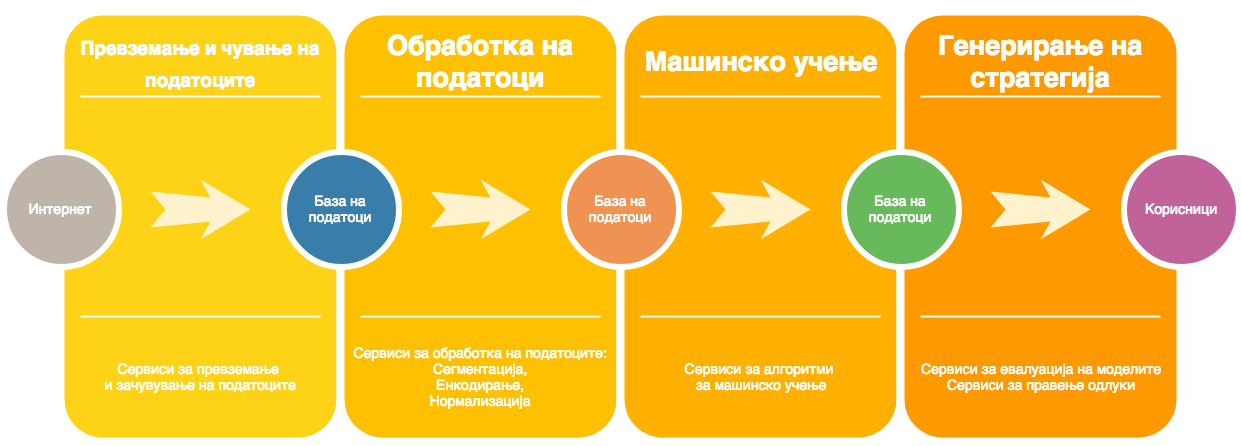
\includegraphics[scale=0.34]{images/Tek_na_podatocite.png}
\caption{Дефинирање на тек на податоци}
\label{fig:tek}
\centering
\end{figure}

\subsection{Справување со тесни грла}
За да можеме системот да го направиме скалабилен прво треба да разгледаме каде би имале тесни грла. Според ограничувањата кои ги разгледавме и апстрактниот дизајн можеме да заклучиме дека најочигледните тесни грла во системот се превземањето на податоците и тренирањето на моделите за машинско учење. За справување со овие проблеми предлагаме паралелизација на роботот за превземање на податоци и паралелизација на тренирањето на моделите. Со тоа системот би изгледал како на слика \ref{fig:system}. Ваквиот дизајн би ги елиминирал очигледните тесни грла кои би се јавиле во системот.

\begin{figure}[hbtp]
\centering
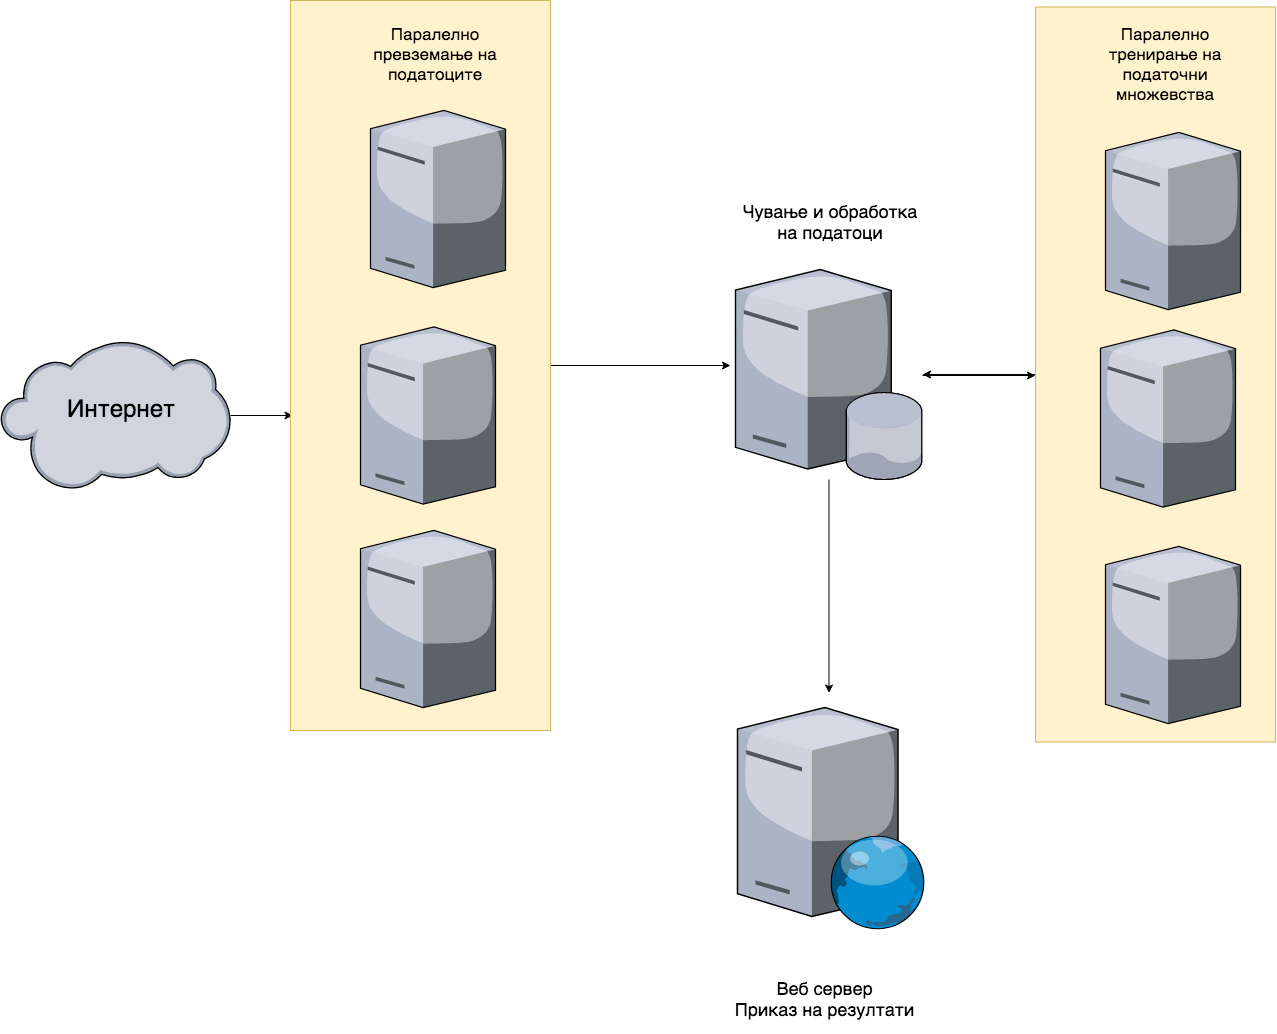
\includegraphics[scale=0.3]{images/system_design.png}
\caption{Дизајн на систем за препораки  за обложување на спортски натпревари}
\label{fig:system}
\end{figure}

\chapter{\mbox{Превземање и обработка на податоци}}
\label{sec:data}
\section{Превземање на податоците}
Алгоритмите за машинско учење учат од податоци. Затоа е важно пред било што во системот да имаме податоци за тренирање на алгоритмите. За нашиот систем одлучивме да користиме податоци од фудбалски натпревари и како едни од главните атрибути ќе ги земеме квотите за обложување доделни од обложувалниците. Постојат повеќе начини на внесување на овој тип на податоци во нашиот систем, но ние ќе се задржиме на три: консумирање на веб сервиси, запишување од датотеки и превземање од интернет страници. Во прилог ќе ги предностите и недостатоците на овие типови на внесувања и кои се нивните предности и недостатоци.  
\subsection{Консумирање на сервиси}
Како еден од најлесните методи на превземање на податоци е консумирањето на веб сервиси. Постојат повеќе платформи што ја нудат оваа опција како за историски податоци така и за податоци во реално време. Бизнис моделот на сите платформи им е продажбата на овие сервиси и бидејќи како што кажавме во првото поглавје обложувањето на спортски натпревари е бизнис од 452 милијарди долари ваквите сервиси се се скапи. Предноста на користење на овој метод за внесување на податоци e тоа што сервисите лесно се конзумираат и податоците се веродостојни. Иако оваа опција од технички аспект е најдобра, од финансиски причини одлучивме за изработката на магистерскиот труд да не ја користиме.  
\subsection{Запишување од датотеки}
Друг метод на внесување на податоци е сериско запишување. Со овој метод е добар за превземање на историските податоци, но не можеме да превземаме податоци во реално време и можно е ограничување на натпреварите на само одредени фудбалски лиги. За нашиот систем ние ги превземавме историските податоци од \cite{football-data} и предноста на овој метод е што податоците се структурирани и може лесно да се внесат во системот. Со овој метод внесовме само 5000 историски податоци за фудбалски натпревари. Останатите податоци го внесуваме преку превземање од интернет страници.
\subsection{Превземање од интернет страници}
Најголемиот дел од податоците што ги внесуваме ви системот е преку превземање од интернет страници. Креиравме робот во Python програмскиот јазик кој прво ги превзема историските податоци од претходните натпревари, а потоа секојдневно превзема податоци за нови натпревари. За развивање на ваквиот софтвер како основа го земавме роботот од \cite{mingov2016application} и го адаптиравме да превзема податоци од неколку веб страници кои прикажуваат податоци за натпревари во реално време. Недостатоците на овој метод на внесување на податоци се дека превземањето и слекцијата на податоците е доста тешка и треба проучување на структурата на веб страната за да можеме да ги одбереме соодветните податоци. Содржината на веб страниците може да биде доста динамична и мала промена на кодот од нивна страна може да влијае на перформансите на роботот. Некои страни ги прикажуваат податоците динамички преку конзумирање на веб сервиси и со тоа се воведува задоцнување. За да се справиме со ваквите проблеми користевме библиотека за автоматизација на веб-прелистувачи \cite{wang2012test} што ги "мами" серверите дека кон нив пристапуваат реални корисници. Со ваквиот начин превземањето на податоците за еден натпревар може да биде во опсег од 3 до 6 секунди. Во претходното поглавје зборувавме за ограничувањата на системот и напоменавме дека постои тесно грло пре превземањето на податоците. Со пресметката од ограничувањата, за превземање на историските податоци потребни се 55 часа, но со паралелизација на повеќе нитки успеавме да превземеме 49000 историски податоци за натпревари за помалку од 10 часа.
\subsection{Чување на податоците}
За да ги зачуваме податоците користиме PostgreSQL \cite{momjian2001postgresql} база на податоци. Податоците од секој натпревар ги внесуваме во табела Натпревар и за секој натпревар чуваме кои тимови играат, во кое време и во која лига, квотите од обложувалниците и резултатите од натпреварот. На слика \ref{fig:eadiagram} е прикажан ЕА дијаграм од базата на податоци, освен Натпревар во системот имаме уште шест табели: Регион, Земја, Лига, Тим, Асоцијација и Спорт. 

\begin{figure}[hbtp]
\centering
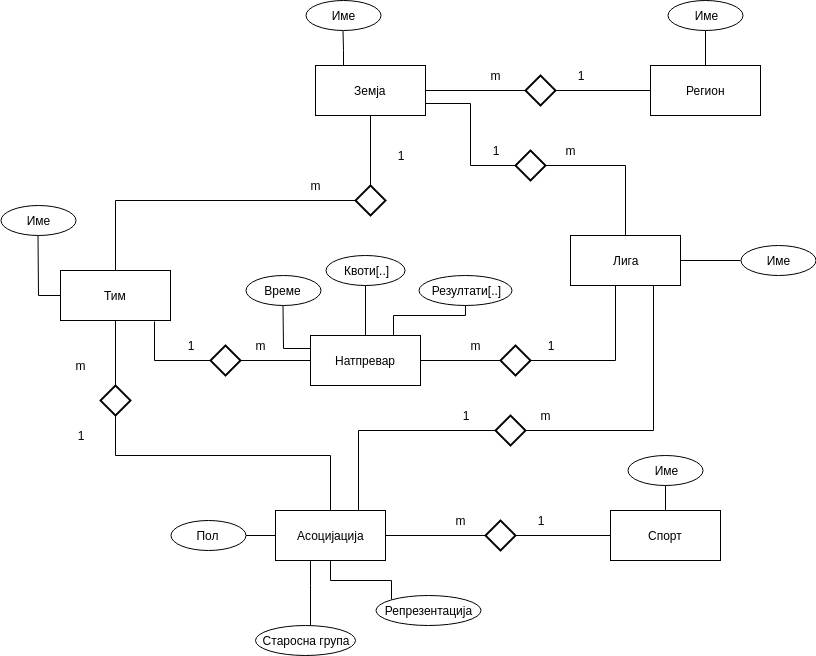
\includegraphics[scale=0.4]{images/EA-diagram.png}
\caption{ЕА дијаграм од базата на податоци}
\label{fig:eadiagram}
\end{figure}

Во табелите Регион и Земја чуваме локациски информации Регион ги соджи континентите во светот, додека Земја ги содржи сите земји. Тим ги содржи сите информации за еден тим, а Лига информациите за лигите во кои се одигруваат натпреварите. Во табелата Асоцијација чуваме податоци за полот и старосната група на еден тим и тоа дали е репрезентација или не. Тимовите може да играат натпревари само во асоцијацијата на која праипаѓаат и во Спорт чуваме податоци на кој спорт припаѓа асоцијацијата.

\section{Обработка и филтрирање}
Многу е важно да ги имаме вистинските податоци за проблемот што сакаме да го решиме. Дури и ако имаме добри податоци, треба да бидеме сигурни дека тие се во корисен формат, скалирани, па дури и дека значајните атрибути се вклучени.
\subsection{Селекција на атрибути}
Целта на овој чекор е да селектираме подмножество од сите достапни податоци со кои ќе работиме. Притоа треба да внимаваме дали некој атрибут има премногу податоци што недостасуваат што би го направиле лош претставник за понатамошната обработка.

Во нашето податочно множество поголемиот дел од атрибутите се обложувачките квоти, освен нив како атрибути ги земаме времето на одигрувањето на натпреварот, тимовите кои се натпреваруваат и лигата во која се натпреваруваат. Со ова податочното множество има 52 атрибути.
\subsection{Изведени атрибути}
Изведени атрибути се атрибути изведени од други податоци користејќи математичка, логичка или некаков друг вид на трансформација.

Во нашиот случај со помош на пребарување врз базата на податоци изведуваме атрибути од резултатите од претходните одиграни натпревари за секој тим како на пример број на дадени голови, број на примени голови. број на победи и порази итн. Освен тоа за секој натпревар вадиме статистика за сите претходни одиграни натпревари меѓу двата тима. Со овие изведени податоци нашето множество вкупно брои 91 атрибут. 
\subsection{Сегментација на множеството}
Сегментацијата на податоците е трансформација која се применува врз дадено множество со цел да добиеме податоци со слични карактеристики. Во нашето множество имаме 54387 натпревари, но ако ја погледнеме нивната распределба на слика \ref{fig:raspredelba} заклучуваме дека повеќето одиграни натпревари се од последните неколку месеци што значи дека имаме мал број на историски податоци што може да ги користиме во тренинг множеството и голем број на нови натпревари што ќе бидат во тест множеството. 
\begin{figure}[hbtp]
\centering
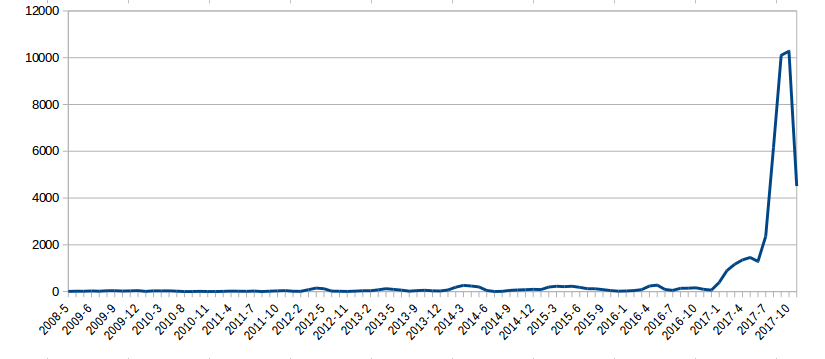
\includegraphics[scale=0.4]{images/raspredelba.png}
\caption{Распределба на одиграни натпревари}
\label{fig:raspredelba}
\end{figure}

Првата сегментација на множеството што ќе ја направиме е сегментација по асоцијација, во предвид ќе ги земеме само натпреварите што имаат асоцијација: мажи, сениори, клупски тимови. Со ваквата трансформација бројот на натпревари се намали на 45743. Поради ваквата распределба на натпреварите и заради тоа што сакаме да ја запазиме хронологијата на податоците, треба да го поделиме множеството на 4 дела: историски податоци, тренинг множество, валидациско множество и тест множество. Историските податоци нема да бидат вклучени во множеството, нив ги занемаруваме со цел да добиеме тренинг множество со добри изведени атрибути. Со тренинг множеството ги тренираме нашите модели, а валидациското множество ќе го користиме при селекција на параметри за моделите. На крај нашите модели ќе ги евалуираме на тест множеството. За нашето истражување направивме 3 групи опсези на поделба на множеството по датуми соодветно. Дополнително вклучивме и уште 4 начини на поделба: сите натпревари, натпревари од тимови кои ги има само во историските и тренинг множества, само тимови кои имаат повеќе од 25 натпревари и тимови кои имаат повеќе од 25 натпревари и ги има само во историските и тренинг множества. Кога ќе ги примениме и трите групи на опсези на овие начини на поделба добиваме 12 множества. За експериментирање одредивме по 4 типа на класификации за секое множество: некој тим ќе победи или е нерешено, домашниот тим победува или не, двата тима ќе поентираат и бројот на голови е парен или непарен.  Со што бројот на множества за тренирање ни се искачи на 48. И последната сегментација што ја применивме е сегментација на натпреварите од само една лига - Англиската премиер лига. Овде не ги применивме опсезите и начините на поделба, во овој случај ја земавме последната сезона да биде тест множество, претпоследната валидациско и останатите 12 сезони како тренинг множество. За оваа сегментација користевме само 2 типа на класификација: некој тим ќе победи или е нерешено, домашниот тим победува или не. Со тоа конечниот број на податочни множества ни достигна до 50. На табела \ref{table:datasets} се прикажани сите изведени множества.

\begin{table}[hbtp]
 \centering
 \scalebox{0.5}{%
 \begin{tabular}{| c | c | c |}
 \hline
 колонa & вредност & опис \\ 
 \hline
 начин & начин 1 & сите натпревари \\
 начин & начин 2 & натпревари од тимови кои ги има само во историските и тренинг множества \\
 начин & начин 3 & само тимови кои имаат повеќе од 25 натпревари \\
 начин & начин 4 & тимови кои имаат повеќе од 25 натпревари и ги има само во историските и тренинг множества \\
 начин & начин 5 & Англиската премиер лига \\
 опсег & опсег 1 & [2014-07-01, 2015-06-30] [2015-07-01, 2016-06-30] [2016-07-01, 2017-11-22] \\
 опсег & опсег 2 & [2015-07-01, 2016-06-30] [2016-07-01, 2017-06-30] [2017-07-01, 2017-11-22] \\
 опсег & опсег 3 & [2016-07-01, 2017-06-30] [2017-07-01, 2017-09-30] [2017-10-01, 2017-11-22] \\
 опсег & опсег 4 & [2004-08-13, 2016-05-16] [2016-08-12, 2017-05-21] [2017-08-10, 2018-02-24]\\
 класа & 1x2 & некој тим ќе победи или е нерешено \\
 класа & 1 or x2 & домашниот тим победува или не \\
 класа & bts &  двата тима ќе поентираат \\
 класа & odd even & бројот на голови е парен или непарен \\
 \hline
\end{tabular}}


\scalebox{0.7}{%
\begin{tabular}{| c | c | c | c | c | c | c | c | }
\hline
број &начин & опсег & класа & тренинг мн. & валидациско мн. & тест мн. & вкупно \\
\hline
 1 & начин 1 & опсег 1 & 1x2 & 891 & 616 & 27052 & 28559\\
 2 & начин 1 & опсег 1 & 1 or x2 & 891 & 616 & 27052 & 28559\\
 3 & начин 1 & опсег 1 & bts & 891 & 616 & 27052 & 28559\\
 4 & начин 1 & опсег 1 & odd even & 891 & 616 & 27052 & 28559\\
 5 & начин 1 & опсег 2 & 1x2 & 616 & 4732 & 22320 & 27668\\
 6 & начин 1 & опсег 2 & 1 or x2 & 616 & 4732 & 22320 & 27668\\
 7 & начин 1 & опсег 2 & bts & 616 & 4732 & 22320 & 27668\\
 8 & начин 1 & опсег 2 & odd even & 616 & 4732 & 22320 & 27668\\
 9 & начин 1 & опсег 3 & 1x2 & 4732 & 12969 & 9351 & 27052\\
 10 & начин 1 & опсег 3 & 1 or x2 & 4732 & 12969 & 9351 & 27052\\
 11 & начин 1 & опсег 3 & bts & 4732 & 12969 & 9351 & 27052\\
 12 & начин 1 & опсег 3 & odd even & 4732 & 12969 & 9351 & 27052\\
 13 & начин 2 & опсег 1 & 1x2 & 891 & 298 & 1146 & 2335\\
 14 & начин 2 & опсег 1 & 1 or x2 & 891 & 298 & 1146 & 2335\\
 15 & начин 2 & опсег 1 & bts & 891 & 298 & 1146 & 2335\\
 16 & начин 2 & опсег 1 & odd even & 891 & 298 & 1146 & 2335\\
 17 & начин 2 & опсег 2 & 1x2 & 616 & 444 & 1347 & 2407\\
 18 & начин 2 & опсег 2 & 1 or x2 & 616 & 444 & 1347 & 2407\\
 19 & начин 2 & опсег 2 & bts & 616 & 444 & 1347 & 2407\\
 20 & начин 2 & опсег 2 & odd even & 616 & 444 & 1347 & 2407\\
 21 & начин 2 & опсег 3 & 1x2 & 4732 & 4878 & 2309 & 11919\\
 22 & начин 2 & опсег 3 & 1 or x2 & 4732 & 4878 & 2309 & 11919\\
 23 & начин 2 & опсег 3 & bts & 4732 & 4878 & 2309 & 11919\\
 24 & начин 2 & опсег 3 & odd even & 4732 & 4878 & 2309 & 11919\\
 25 & начин 3 & опсег 1 & 1x2 & 338 & 155 & 2828 & 3321\\
 26 & начин 3 & опсег 1 & 1 or x2 & 338 & 155 & 2828 & 3321\\
 27 & начин 3 & опсег 1 & bts & 338 & 155 & 2828 & 3321\\
 28 & начин 3 & опсег 1 & odd even & 338 & 155 & 2828 & 3321\\
 29 & начин 3 & опсег 2 & 1x2 & 155 & 1195 & 1633 & 2983\\
 30 & начин 3 & опсег 2 & 1 or x2 & 155 & 1195 & 1633 & 2983\\
 31 & начин 3 & опсег 2 & bts & 155 & 1195 & 1633 & 2983\\
 32 & начин 3 & опсег 2 & odd even & 155 & 1195 & 1633 & 2983\\
 33 & начин 3 & опсег 3 & 1x2 & 1195 & 1100 & 533 & 2828\\
 34 & начин 3 & опсег 3 & 1 or x2 & 1195 & 1100 & 533 & 2828\\
 35 & начин 3 & опсег 3 & bts & 1195 & 1100 & 533 & 2828\\
 36 & начин 3 & опсег 3 & odd even & 1195 & 1100 & 533 & 2828\\
 37 & начин 4 & опсег 1 & 1x2 & 338 & 101 & 618 & 1057\\
 38 & начин 4 & опсег 1 & 1 or x2  & 338 & 101 & 618 & 1057\\
 39 & начин 4 & опсег 1 & bts  & 338 & 101 & 618 & 1057\\
 40 & начин 4 & опсег 1 & odd even  & 338 & 101 & 618 & 1057\\
 41 & начин 4 & опсег 2 & 1x2 & 155 & 225 & 576 & 956\\
 42 & начин 4 & опсег 2 & 1 or x2 & 155 & 225 & 576 & 956\\
 43 & начин 4 & опсег 2 & bts & 155 & 225 & 576 & 956\\
 44 & начин 4 & опсег 2 & odd even & 155 & 225 & 576 & 956\\
 45 & начин 4 & опсег 3 & 1x2 & 1195 & 1058 & 512 & 2765\\
 46 & начин 4 & опсег 3 & 1 or x2 & 1195 & 1058 & 512 & 2765\\
 47 & начин 4 & опсег 3 & bts & 1195 & 1058 & 512 & 2765\\
 48 & начин 4 & опсег 3 & odd even & 1195 & 1058 & 512 & 2765\\
 49 & начин 5 & опсег 4 & 1x2 & 4560 & 380 & 279 & 5219 \\
 50 & начин 5 & опсег 4 & 1 or x2 & 4560 & 380 & 279 & 5219 \\
\hline
\end{tabular}}
\caption{Изведени множества за тренирање}
\label{table:datasets}
\end{table}

\section{Трансформација на податоците}
Последниот чекор што ќе го превземеме при обработката на податоците е трансформацијата. Алгоритмите со којшто ќе работиме и доменот на проблемот ќе влијаат на овој чекор и многу веројатно ќе треба да ги ревидираме различните трансформации на нашите препроцесирани податоци додека работиме на нашиот проблем.
\subsection{Кодирање}
Кодирање или продолжување е трансформација на категорични променливи на бинарни или нумерички. Категориските променливи мора да бидат кодирани во многу методи за моделирање. Два главни типа на кодирање се бинарно и класно.

\subsubsection{Бинарно кодирање}
Нумерирање на категориски променливи со земање на вредности 0 или 1 за да укаже на отсуство или присуство на секоја категорија. Ако категориската променлива има k категории, ќе треба да создадеме k бинарни променливи. Главниот недостаток со овој метод е кога категориска променлива со многу вредности (на пример, тимови), која може значително да ја зголеми димензијата на податоците. Во нашиот случај овој тип на кодирање можеме да го примениме само во множествата под број 49 и 50 од табела \ref{table:datasets}. Во другите множества бројот на тимови е поголем и со тоа може значитено да се зголеми бројот на атрибути.
\subsubsection{Класно кодирање}
Класното кодирање е нумерирање на категорични променливи преку класата. Во овој метод, ние ја заменуваме категориската променлива со само една нова нумеричка променлива и ја заменуваме секоја категорија на категориска променлива со соодветната веројатност на класата. Главните недостатоци на овој метод се нејзината зависност од дистрибуцијата на класата и нејзината пониска моќ на предвидување во споредба со бинарниот метод на кодирање.
\subsection{Нормализација}
Откако ќе ги трансформираме сите податоци на множеството во нумерички потребно е да направиме скалирање на податоците во даден опсег овој процес се вика нормализација. За нашиот проблем ние ќе примениме две различни нормализации: нормализација по стандардна девијација и min-max нормализација во опсег од 0 до 1. 
\section{Обработени податоци и следни чекори}
Во ова поглавје ги разгледавме чекорите за превземање и обработка на податоците, увидовме на потребните чекори потребни за да направиме добри множества и како да ги трансформираме податоците за да можеме да добиваме подобри резултати со алгоритмите за машинско учење. Во следното поглавје ќе рагледаме дел од нив.    
\chapter{Алгоритми за машинско учење}
\label{sec:machine_learning}
Постојат многу алгоритми за машинско учење и ако би ги именувале сите би изгледале премногу и не би знаеле да одбереме соодветен доколку не би направеле некакво групирање. Најчести групирања со кои можеме да се сретнеме се групирање по сличност по форма и функција и групирање по начин на учење. И двата пристапи се корисни, но ќе се фокусираме групирањето по начин на учење со цел да најдеме соодветни алгоритми за решавање на начиот проблем. 
Постојат различни начини на кои алгоритам може да се моделира проблем врз основа на неговата интеракција со искуството или околината или она што сакаме да го наречеме влезни податоци.
Популарно е во машинското учење да се разгледаат начините за учење кои еден алгоритам може да го усвои.
Постојат само неколку главни начини на учење или модели за учење кои еден алгоритам може да ги има: надгледувано учење, ненадгледувано учење и полу-надгледувано учење.
Оваа таксономија или начинот на организирање алгоритми за машинско учење е корисна затоа што не да размислуваме за улогите на влезните податоци и за процесот на подготовка на модел и одбереме оној кој е најсоодветен за нашиот проблем за да го добиете најдобриот резултат.

Кај надгледуваното учење влезните податоци се нарекуваат тренинг податоци и имаат позната класа или резултат како што се спам / не-спам или цената на акциите во одредено време.
Моделот се подготвува преку процес на обука во кој е потребно да се направат предвидувања и се корегира кога тие предвидувања се погрешни. Процесот на обука продолжува додека моделот не постигне посакувано ниво на точност на податоците за обуката.
Проблеми кои се решаваат со надгледуваното учење се класификација и регресија.

Кај ненадгледуваното учење влезните податоци не се етикетирани и немаат познат резултат.
Моделот се подготвува со издвојување на структури присутни во влезните податоци. На овој начин може да се извлечат општи правила за податоците. Тоа може да биде преку математички процес, или може да биде да се организираат податоци по сличност.
Проблеми кои се решаваат со ненадгледуваното учење се кластерирање, намалување на димензионалноста и учење на правила за здружување.

Кај полу-надгледуваното учење влезните податоци се мешавина од етикетирани и неетикетирани примери.
Овде моделот мора да ги научи структурите за организирање на податоците, како и да направи предвидувања.
Проблеми кои се решаваат со надгледуваното учење се исто така класификација и регресија.

Во нашиот случај треба да решиме проблем на класифицирање и имаме познати класи за сите влезни податоци, затоа проблемот ќе го дефинираме како надгледувано учење. Пред да се врутниме кон решавање на проблемот со помош на вештачки невронски мрежи, ќе разгледаме неколу алгоритми за надгледувано учење и како тие го решаваат нашиот проблем.  
\section{Алгоритми за надгледувано учење}
\subsection{Наивен баесов класификатор}
Наивниот баесов класификатор \cite{rish2001empirical} е класификациски алгоритам за бинарни и повеќе-класни класификациски проблеми.
Се нарекува наивен баесов класификатор, бидејќи пресметката на веројатностите за секоја хипотеза се поедноставени за да се направи нивната пресметка попрактична. Наместо да се обидуваат да ги пресметаат вредностите на секоја вредност на атрибутот P (d1, d2, d3 | h), се претпоставува дека се условно независни со оглед на целните вредности и се пресметуваат како P (d1 | h) * P (d2 | H) и и така натаму.
Ова е многу силна претпоставка која е малку веројатна кај реалните проблеми, односно дека атрибутите не си влијаат еден на друг.

На сликa \ref{fig:naive_bayes} се прикажани резултатите од тестирањето на сите податочни множества со наивен баесов класификатор поделени по класа. Најдобри резултати овој алгоритам постигнува кај множествата 49 и 50 дефинирани во табела \ref{table:datasets}, со 54.83\% за класифицирање на 1 Х 2 игра, односно 67.38\% за класифицирање на 1 или Х2 игра. 

\begin{figure}[H]
\centering
\begin{tabular}{cc}
  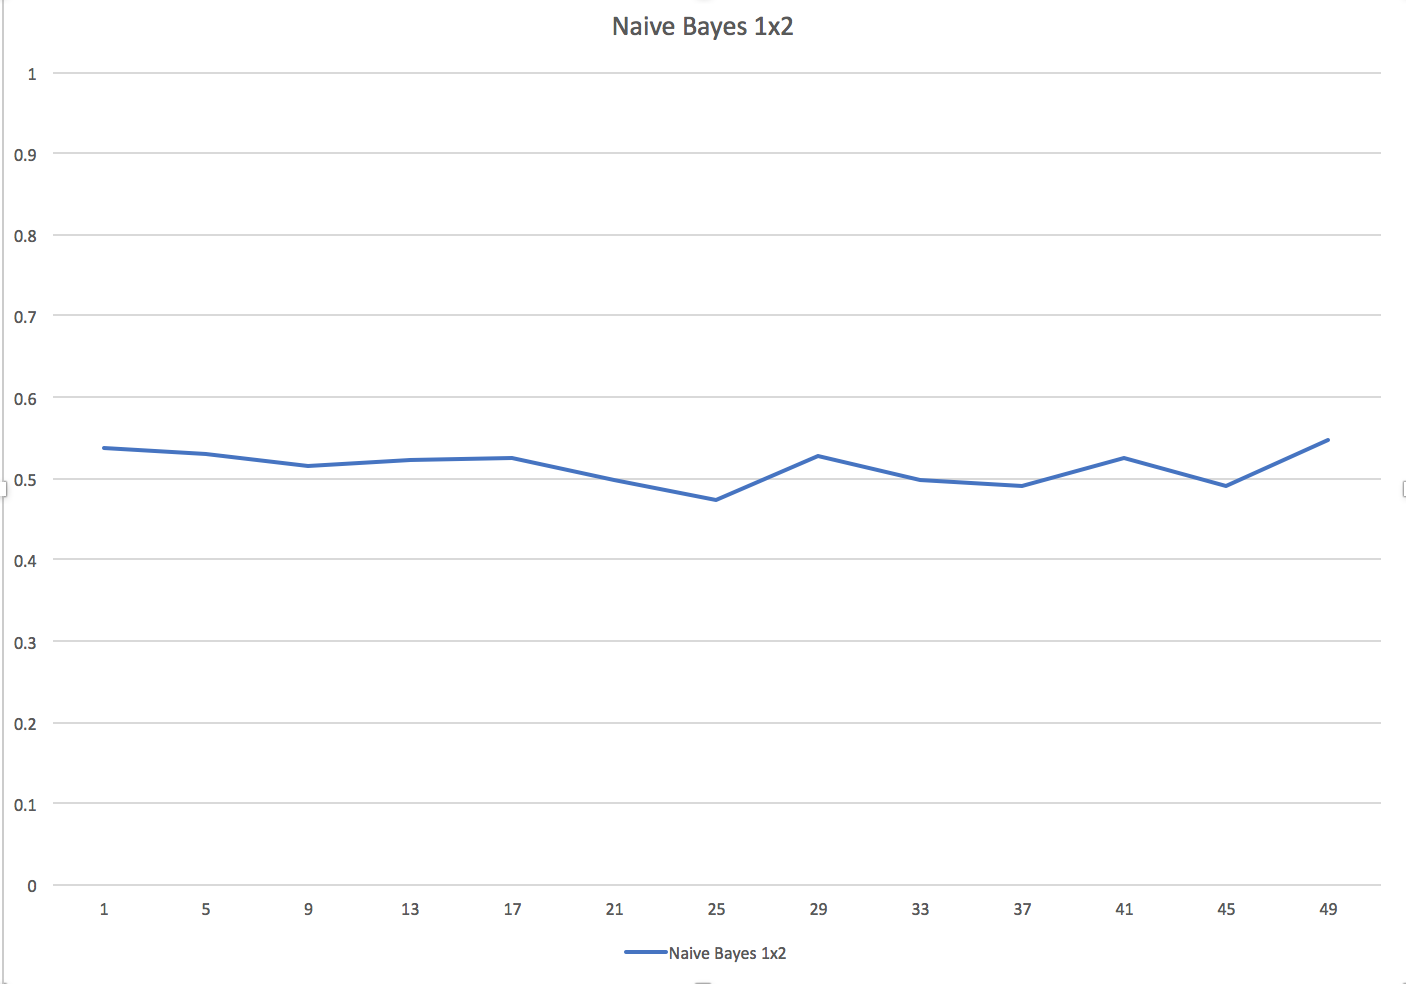
\includegraphics[width=8cm,height=5cm]{images/naive_bayes_1x2.png} &   
  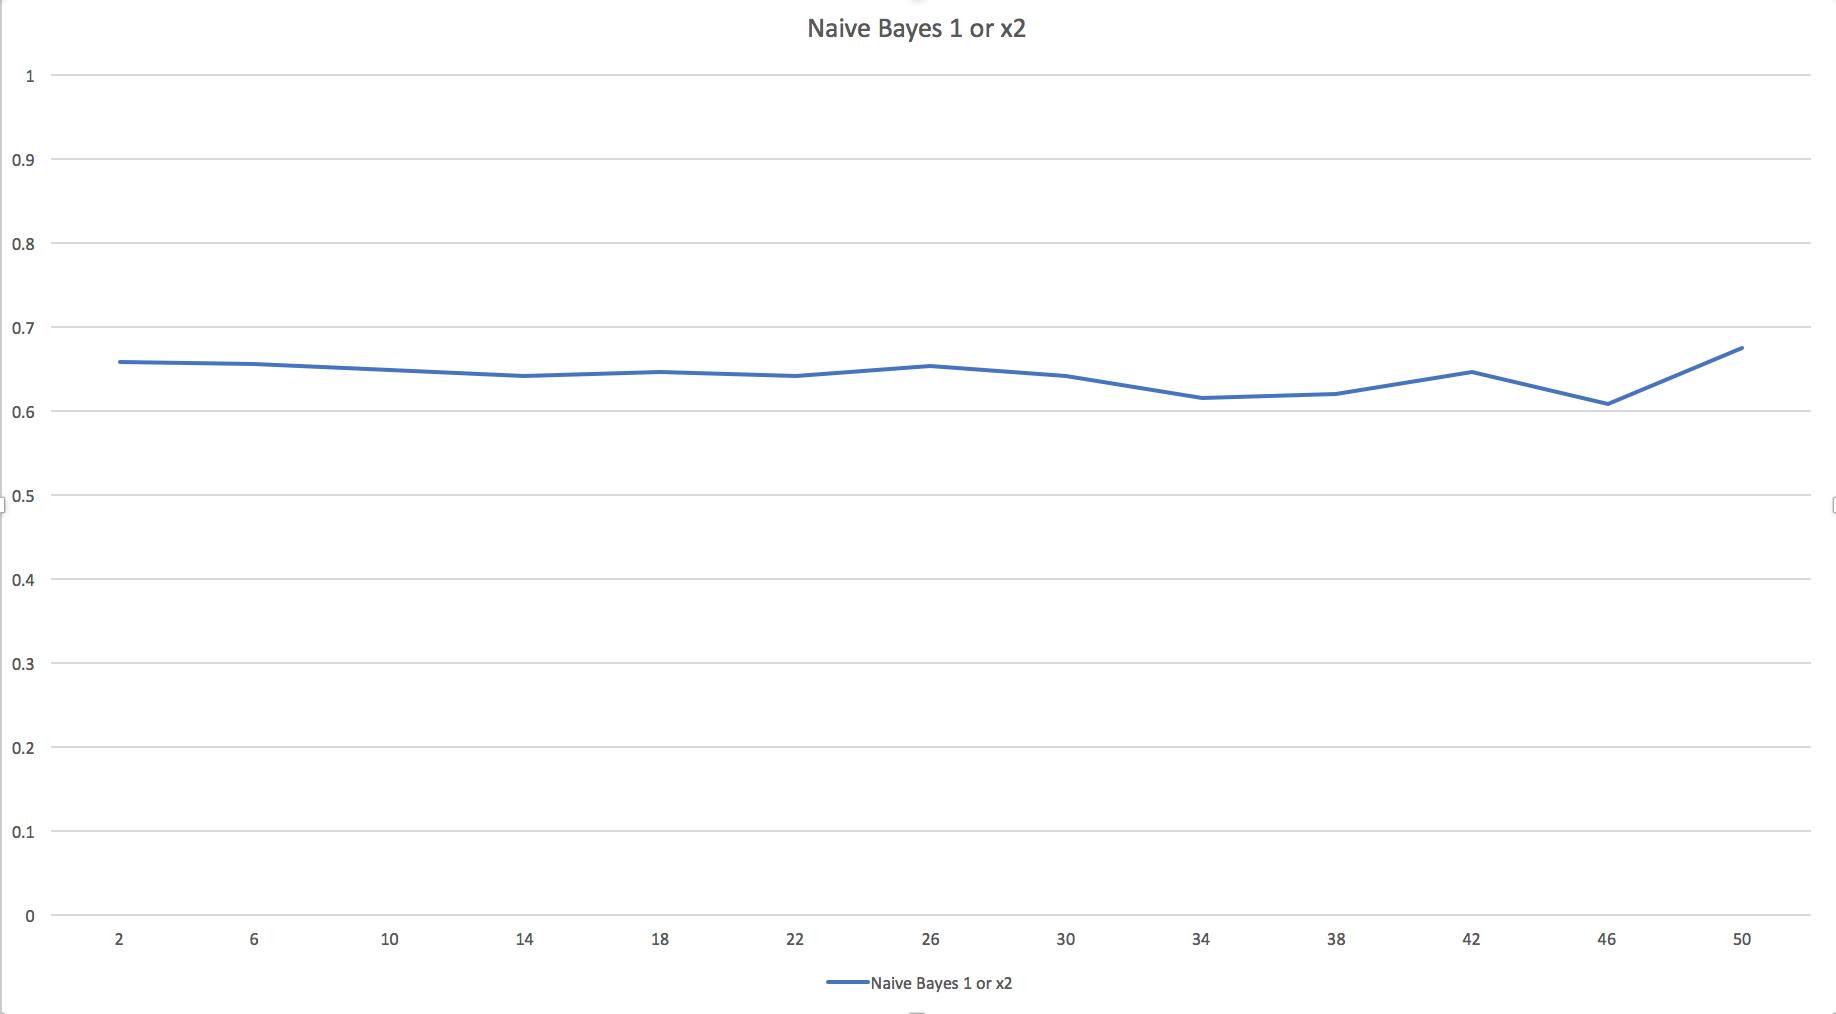
\includegraphics[width=8cm,height=5cm]{images/naive_bayes_1_or_x2.png} \\
(а) 1 Х 2 & (б) 1 или Х2 \\
 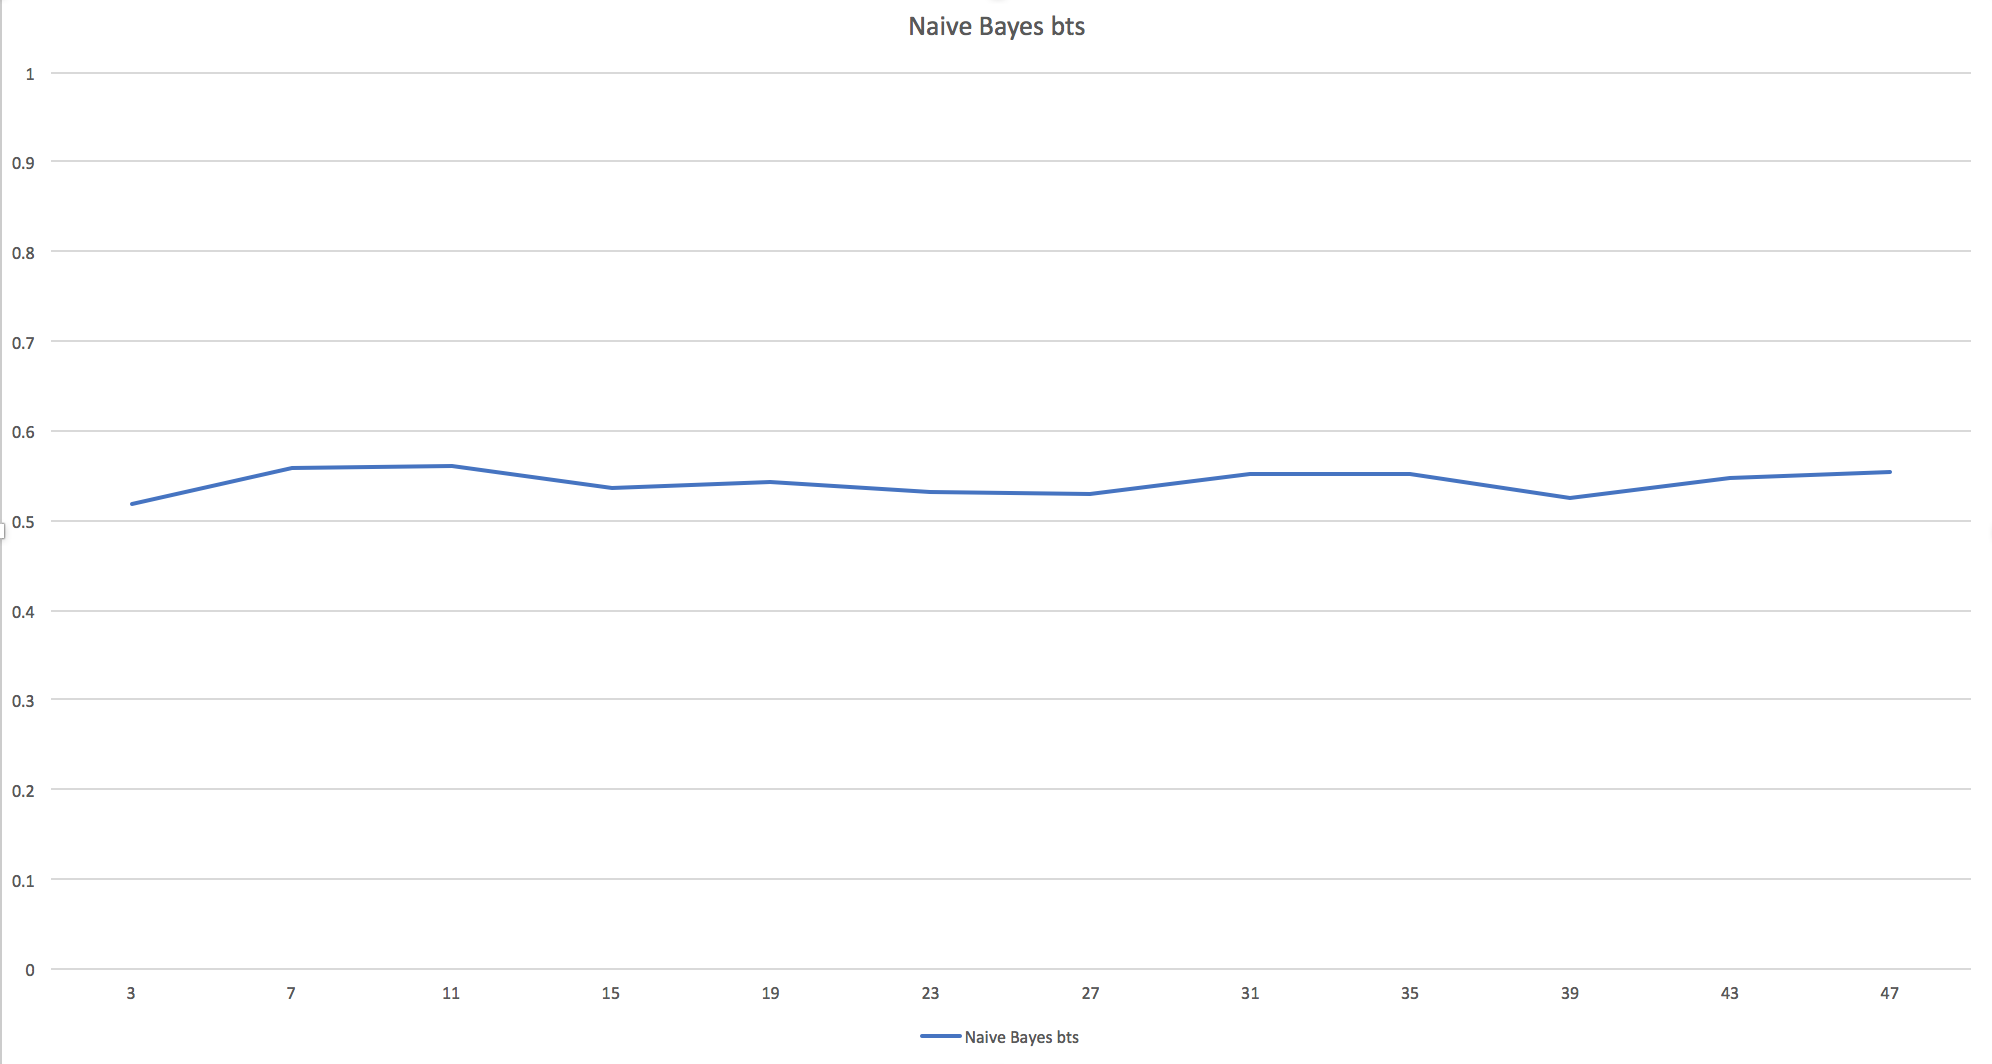
\includegraphics[width=8cm,height=5cm]{images/naive_bayes_bts.png}
 &   
 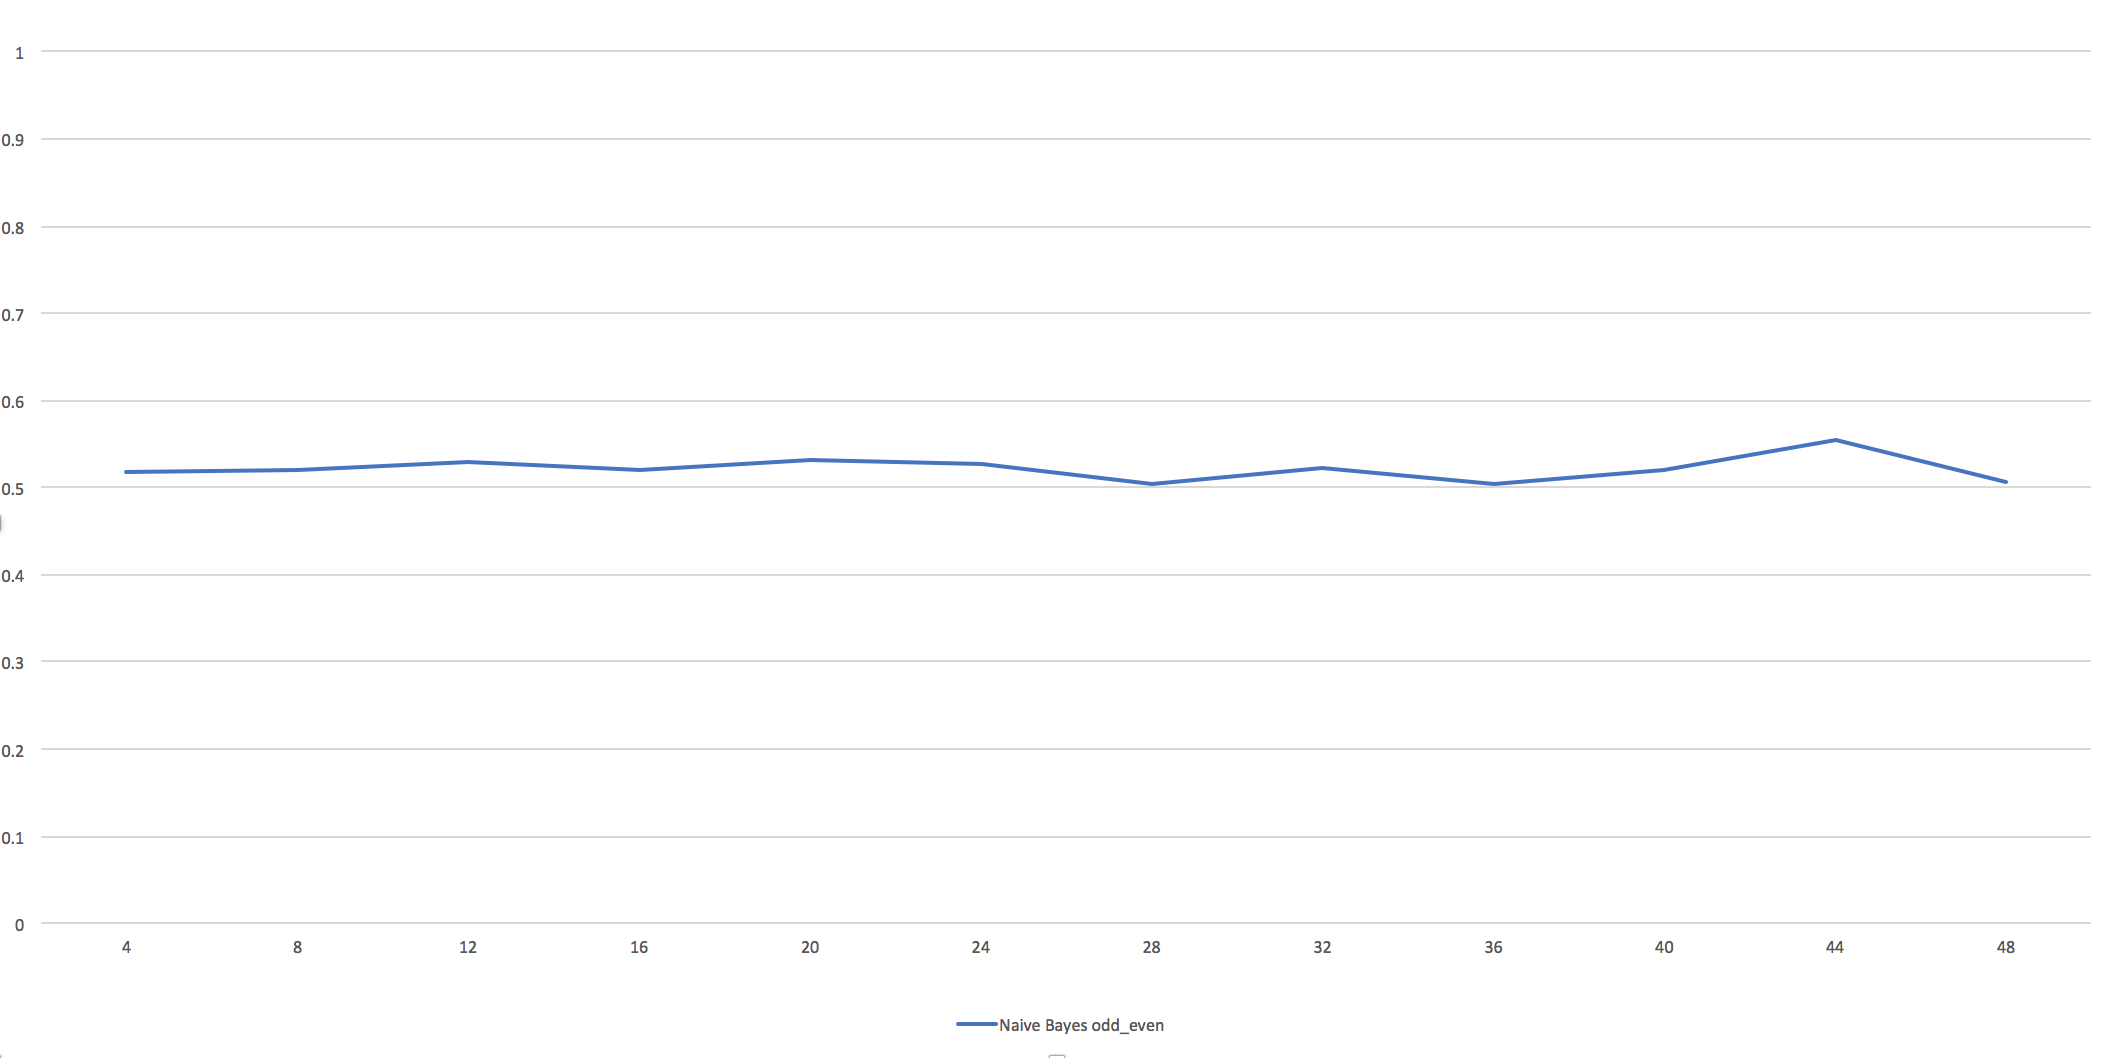
\includegraphics[width=8cm,height=5cm]{images/naive_bayes_odd_even.png} \\
(в) дали двата тима ќе поентираат & (г) парен/непарен број на голови \\
\end{tabular}
\caption{Резултати од тестирање со наивен баесов класификатор}
\label{fig:naive_bayes}
\end{figure}

\subsection{Логистичка регресија}
Логистичката регресија \cite{hosmer2013applied}, и покрај неговото име, е линеарен модел за класификација наместо регресија. Логистичката регресија е позната во литературата и како класификација на максимална ентропија или лог-линеарен класификатор. Во овој модел, веројатностите што ги опишуваат можните исходи на едно испитување се моделираат со помош на логистичка функција.
Логистичката функција, исто така наречена сигмоидна функција, била развиена од страна на статистичарите за да ги опише својствата на растот на популацијата во екологијата. Тоа е крива во форма на Ѕ (лат.), која може да земе реален број и да ја прикаже неговата вредност помеѓу 0 и 1.

На сликa \ref{fig:log_reg} се прикажани резултатите од тестирањето на сите податочни множества со логистичка регресија поделени по класа. Најдобри резултати овој алгоритам постигнува кај множествата 49 и 50 дефинирани во табела \ref{table:datasets}, со 54.83\% за класифицирање на 1 Х 2 игра, односно 67.74\% за класифицирање на 1 или Х2 игра.

\begin{figure}[H]
\centering
\begin{tabular}{cc}
  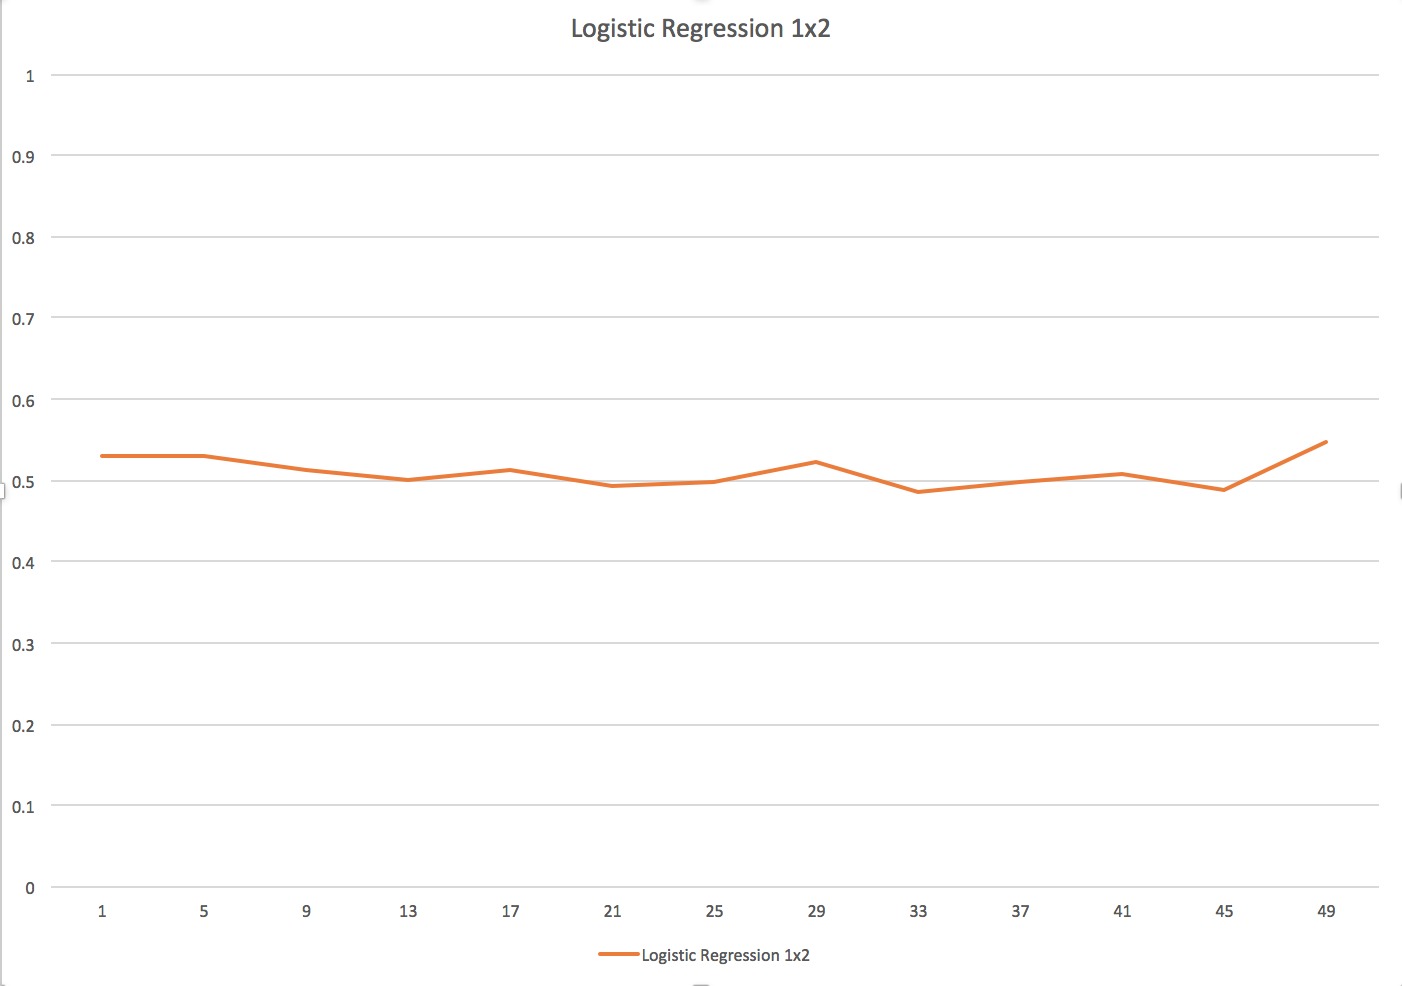
\includegraphics[width=8cm,height=5cm]{images/log_reg_1x2.png} &   
  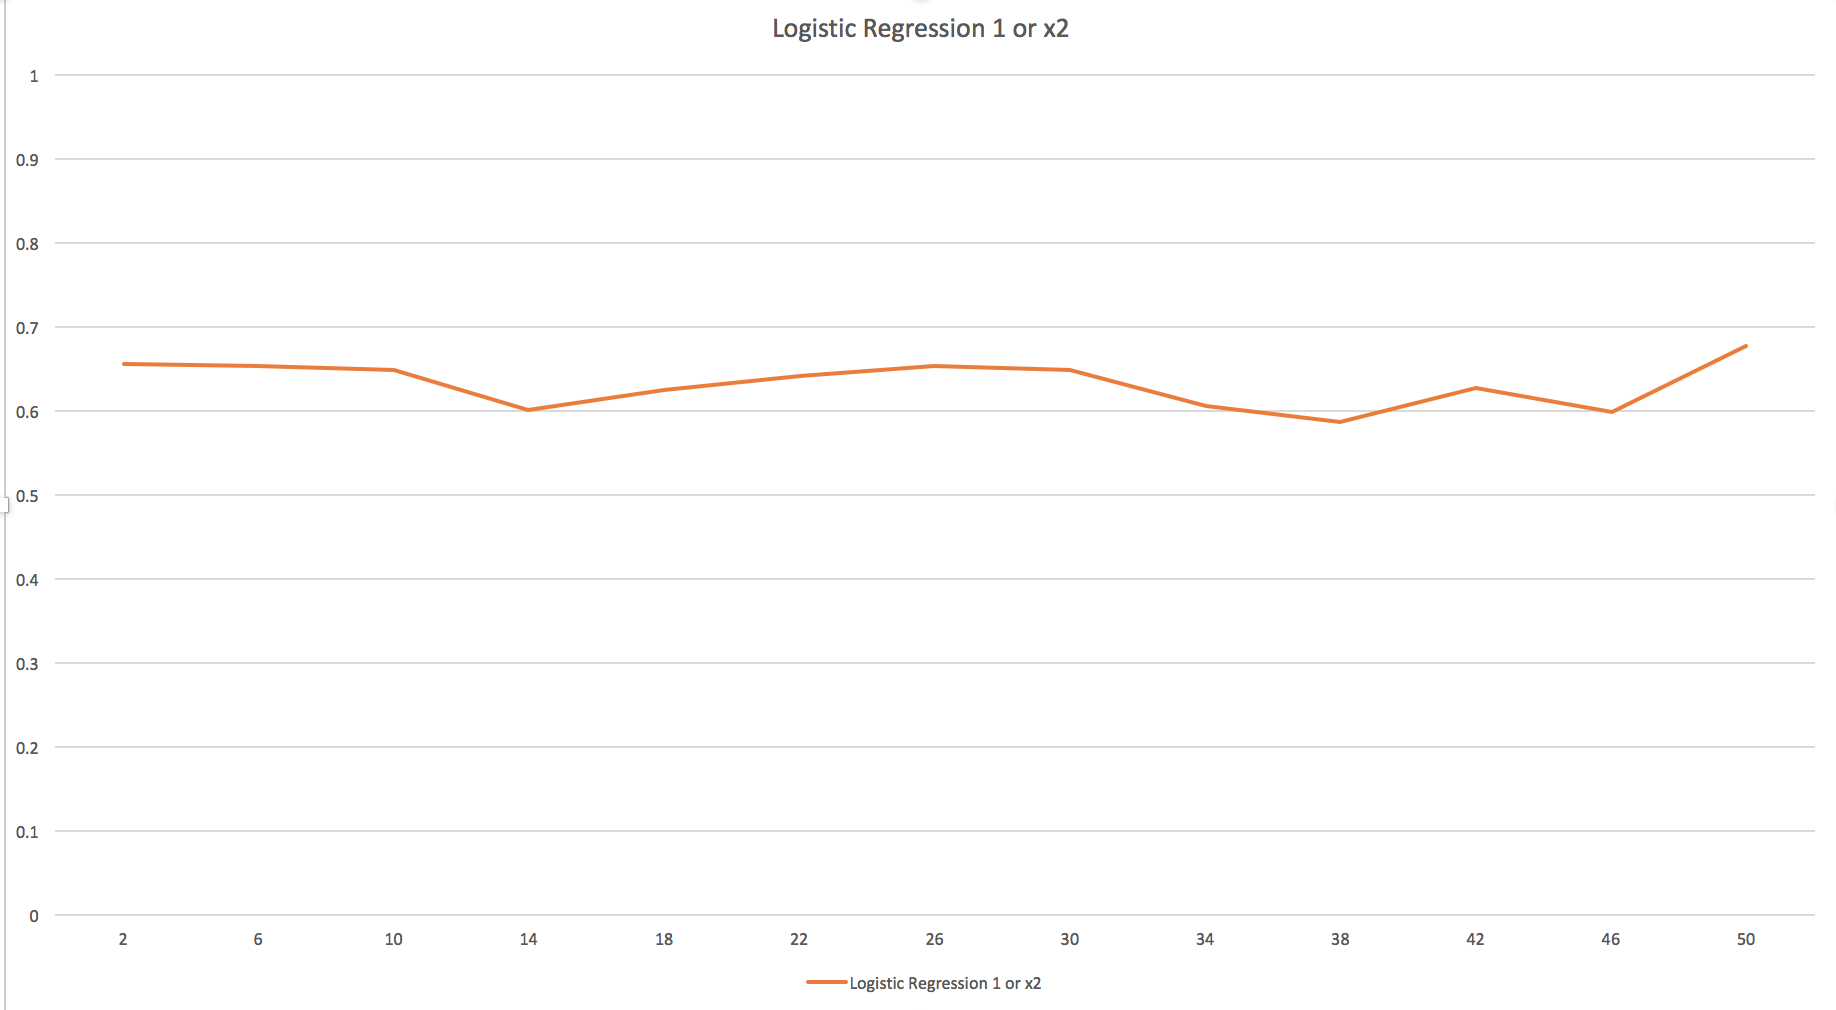
\includegraphics[width=8cm,height=5cm]{images/log_reg_1_or_x2.png} \\
(а) 1 Х 2 & (б) 1 или Х2 \\
 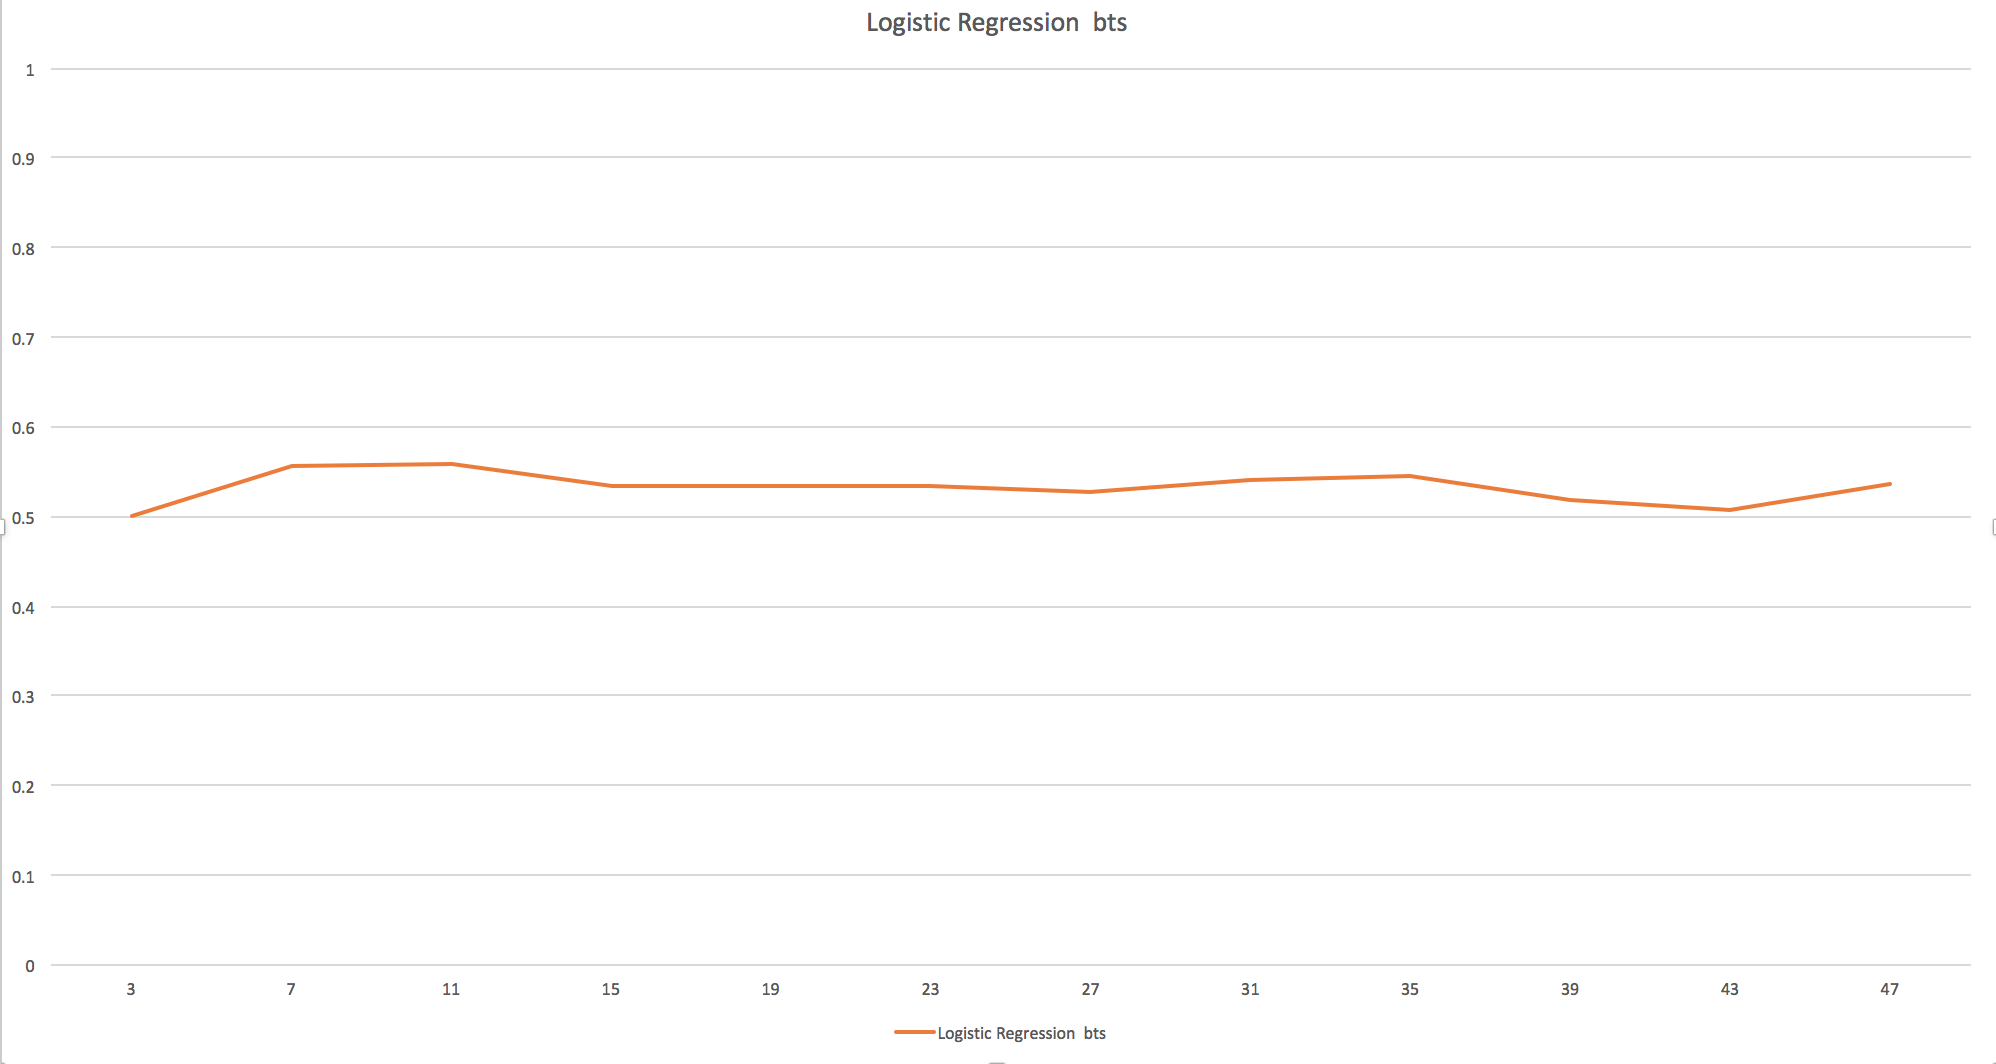
\includegraphics[width=8cm,height=5cm]{images/log_reg_bts.png}
 &   
 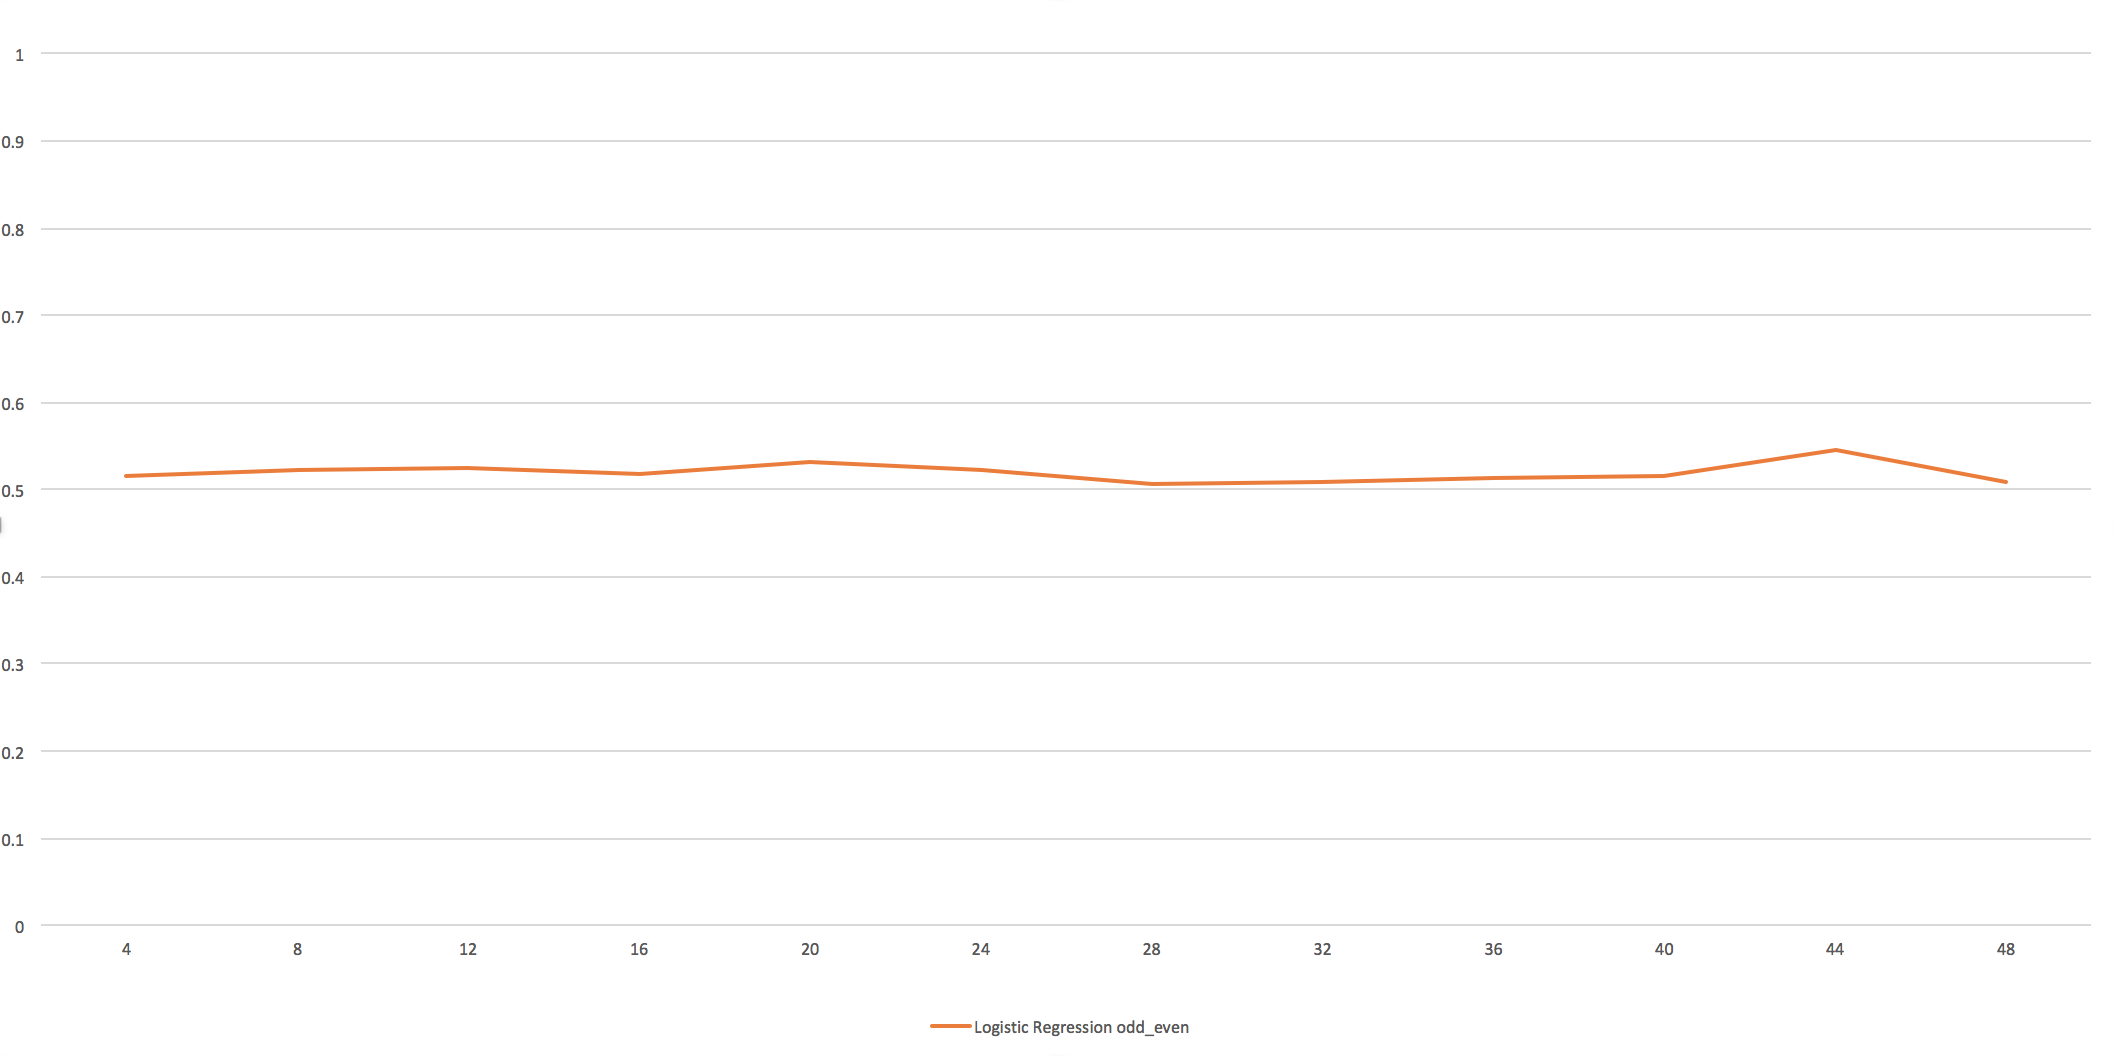
\includegraphics[width=8cm,height=5cm]{images/log_reg_odd_even.png} \\
(в) дали двата тима ќе поентираат & (г) парен/непарен број на голови \\
\end{tabular}
\caption{Резултати од тестирање со логистичка регресија}
\label{fig:log_reg}
\end{figure}

\subsection{Машини со носечки вектори}
Машини со носечки вектори SVM (анг.) \cite{cortes1995support} е можеби еден од најпопуларните алгоритми за машинско учење \cite{lameski2015svm, zdravevski2015robust}.
SVM класифицира податоци со наоѓање на најдобра хиперрамнина која ги одделува сите податоци точки од една класа од оние на другата класа. Најдобра хиперрамнина за SVM значи онаа со најголема маргина меѓу двете класи. Маргината значи максимална ширина на просторот паралелен на хиперпамнината кој нема внатрешни податоци.

На сликa \ref{fig:svm} се прикажани резултатите од тестирањето на сите податочни множества со машини со носечки вектори поделени по класа. Најдобри резултати овој алгоритам постигнува кај множествата 49 и 50 дефинирани во табела \ref{table:datasets}, со 55.19\% за класифицирање на 1 Х 2 игра, односно 67.38\% за класифицирање на 1 или Х2 игра.

\begin{figure}[H]
\centering
\begin{tabular}{cc}
  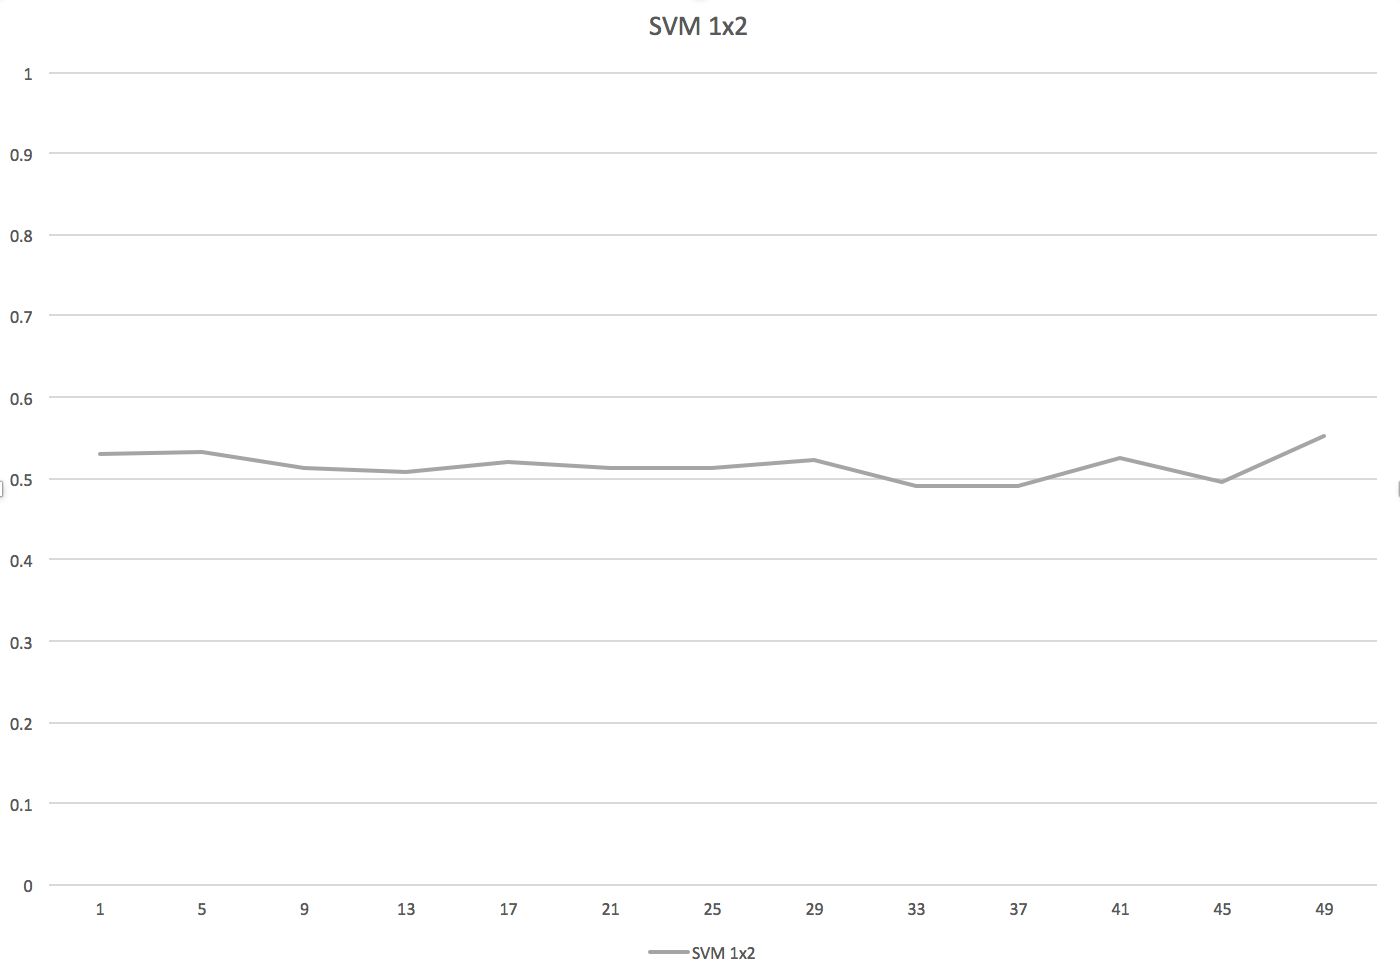
\includegraphics[width=8cm,height=5cm]{images/svm_1x2.png} &   
  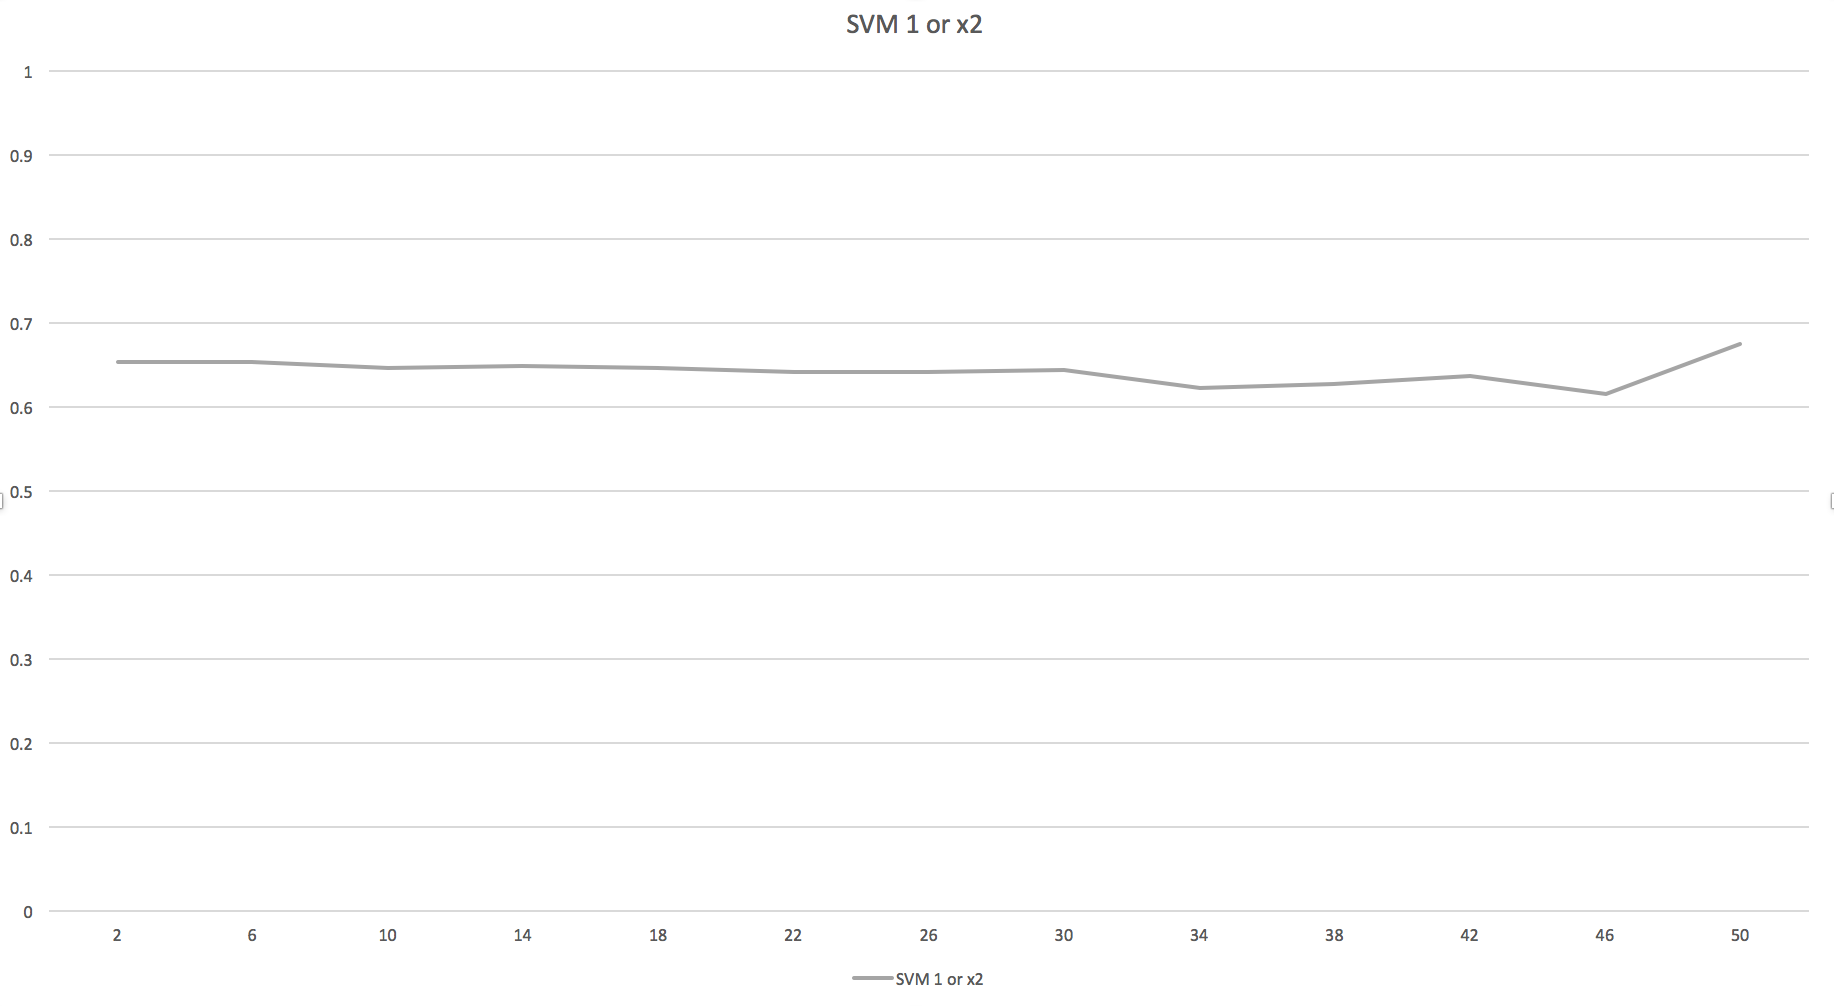
\includegraphics[width=8cm,height=5cm]{images/svm_1_or_x2.png} \\
(а) 1 Х 2 & (б) 1 или Х2 \\
 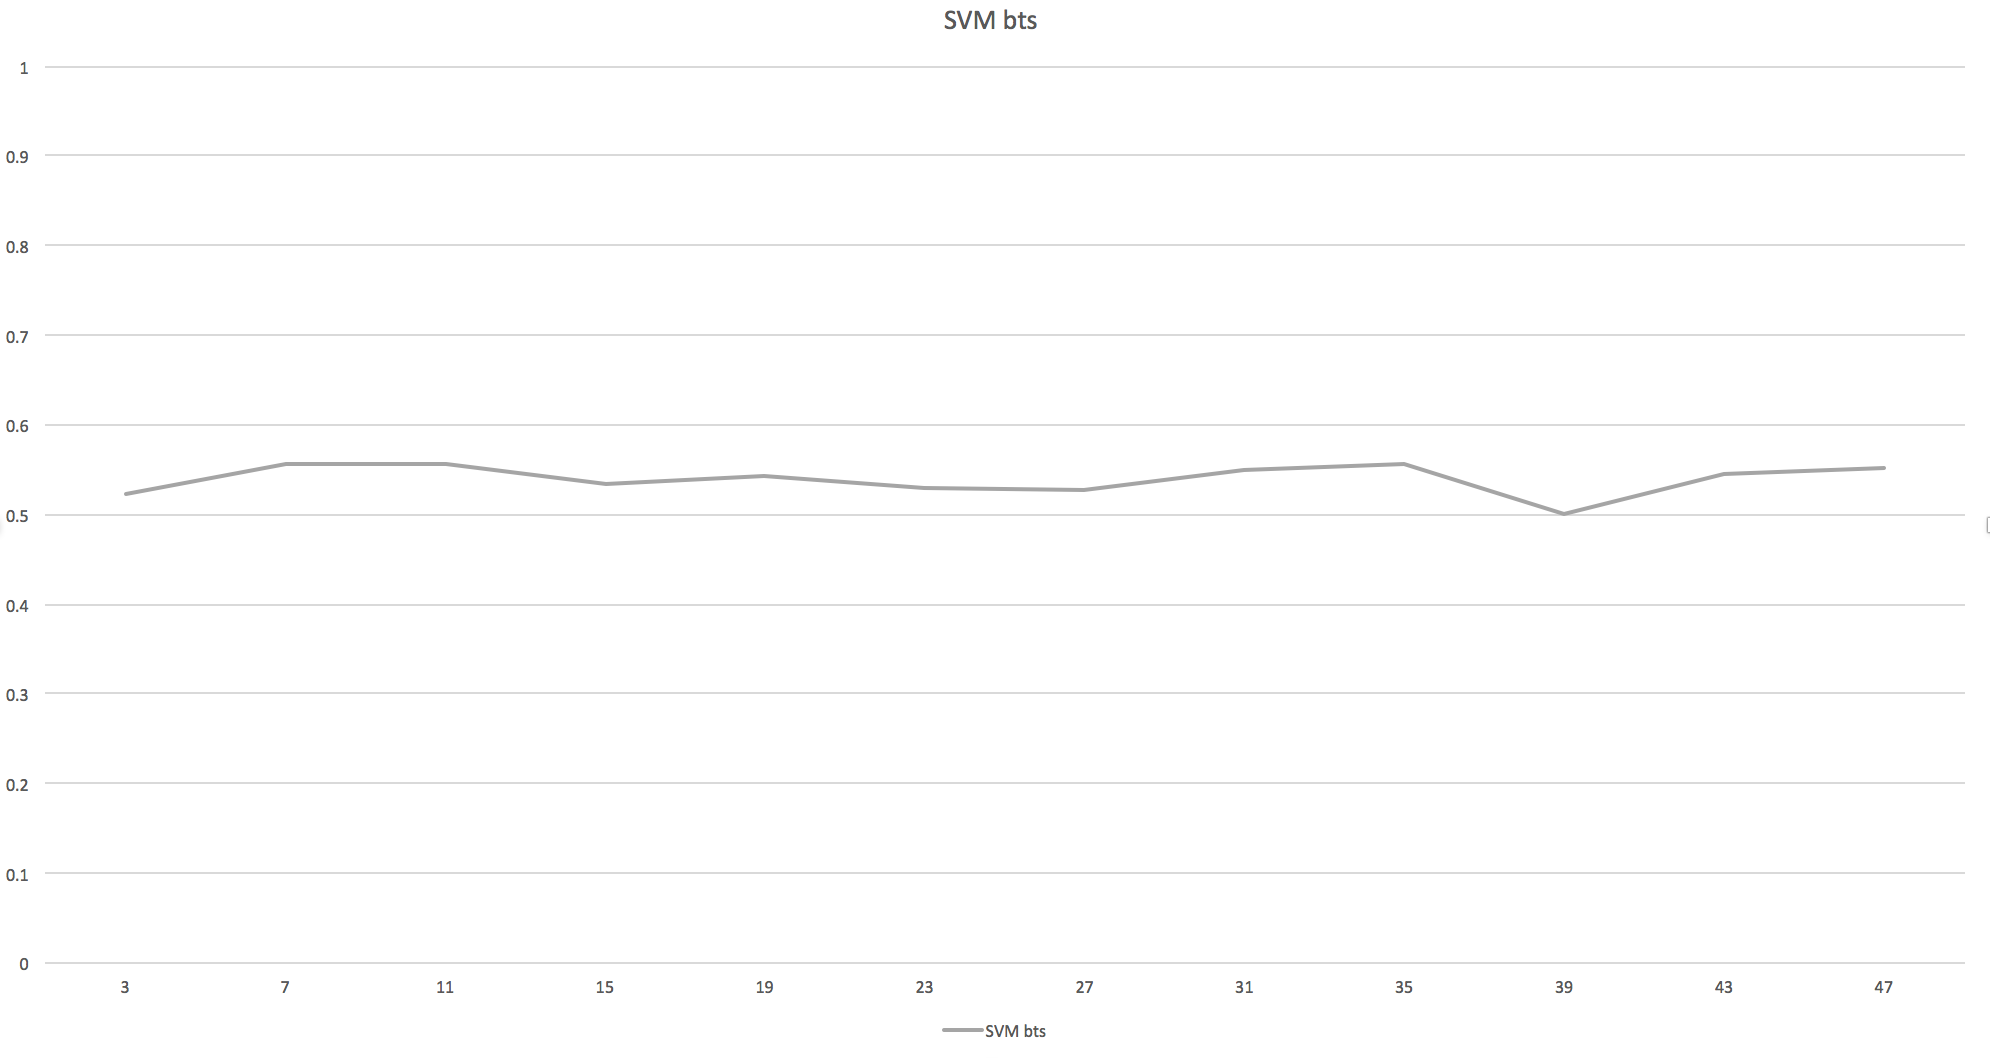
\includegraphics[width=8cm,height=5cm]{images/svm_bts.png}
 &   
 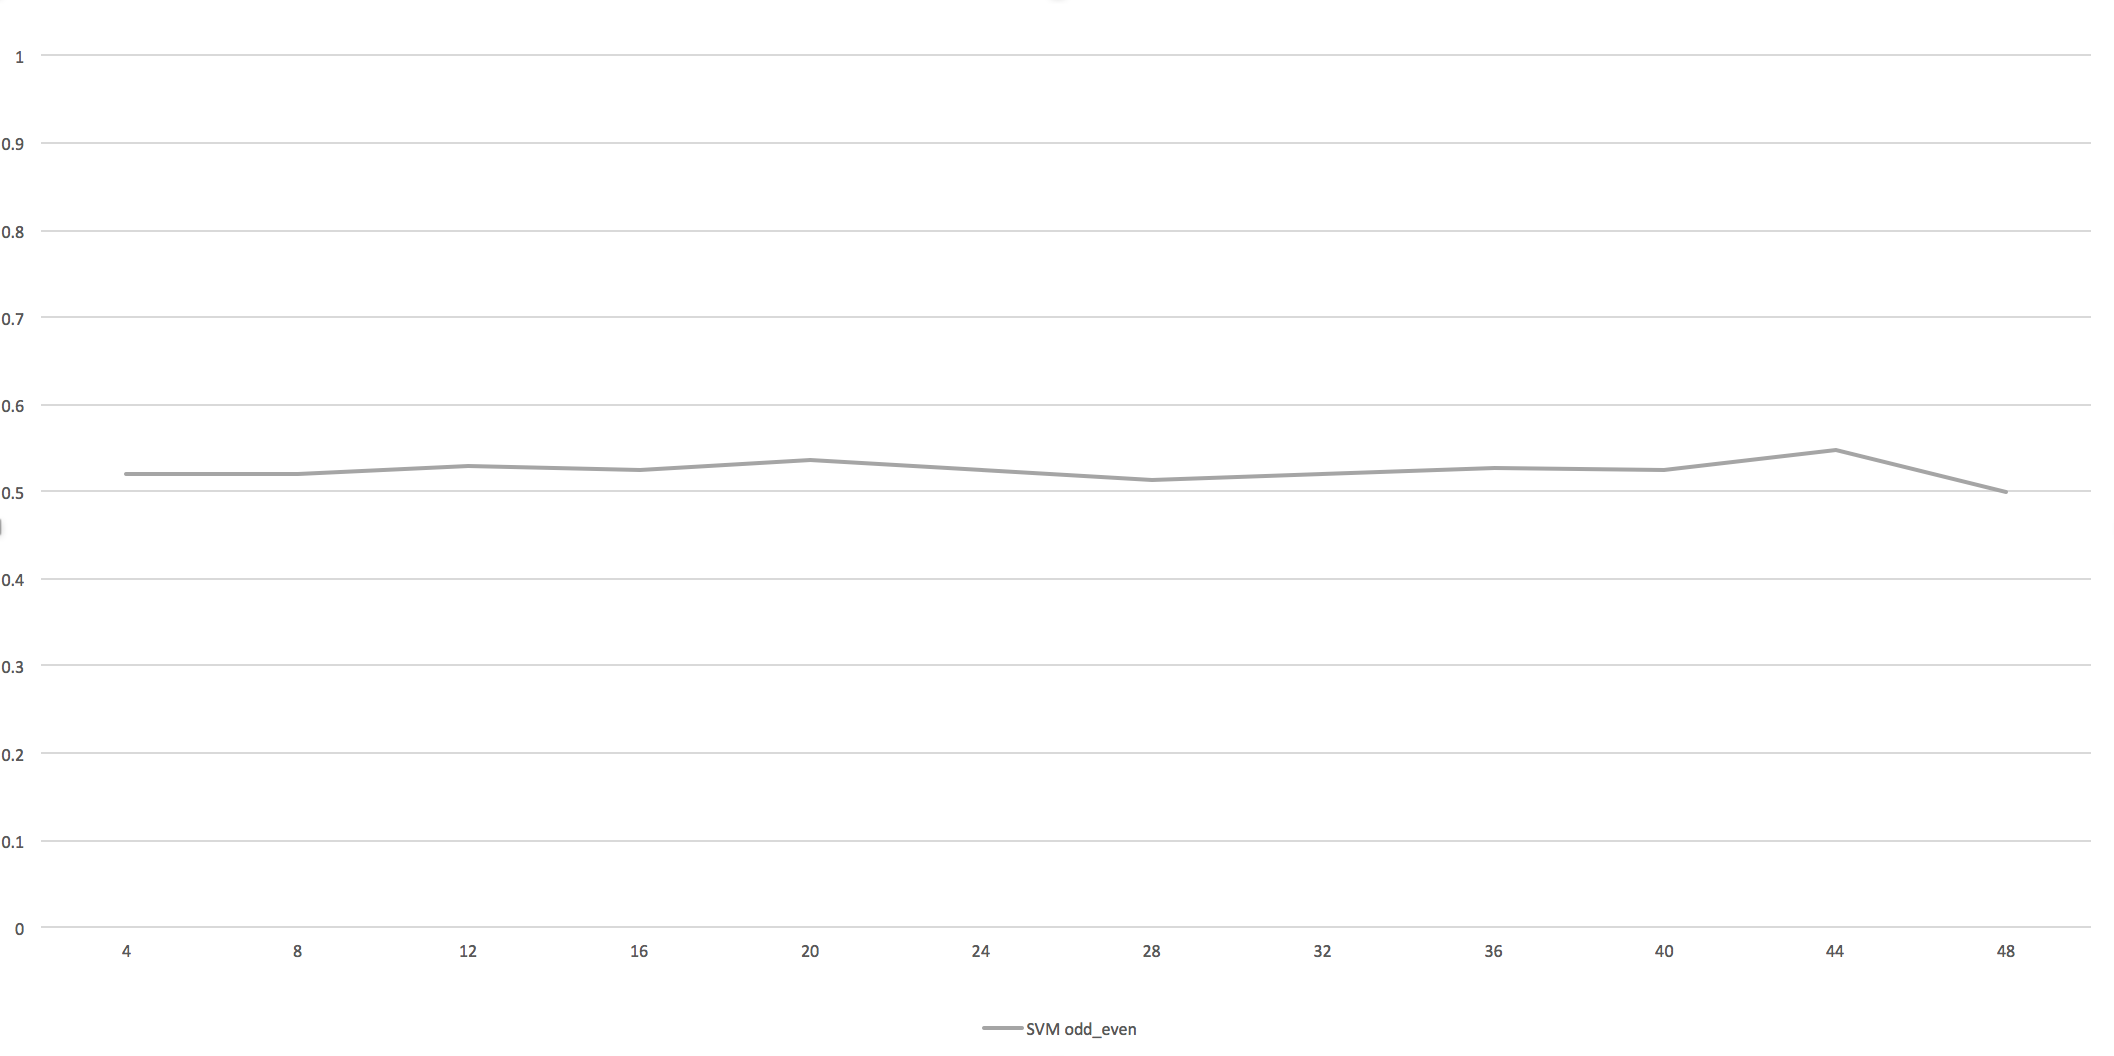
\includegraphics[width=8cm,height=5cm]{images/svm_odd_even.png} \\
(в) дали двата тима ќе поентираат & (г) парен/непарен број на голови \\
\end{tabular}
\caption{Резултати од тестирање со машини со носечки вектори}
\label{fig:svm}
\end{figure}

\subsection{Случаjни шуми}
Случаjни шуми \cite{breiman2001random} е еден од најпопуларните и најмоќните алгоритми за машинско учење. Тоа е еден вид алгоритам за учење на машина за ансамбли, кој комбинира инидивидуални класификатори со цел да се подобрат неговите перформанси.
Во случајни шуми, секое дрво во ансамблот е изградено од примерок составен со замена од сетот за обука. Покрај тоа, при разделување на јазол за време на изградбата на дрвото, поделбата што е избрана повеќе не е најдобрата поделба меѓу сите карактеристики. Наместо тоа, поделбата што е избрана е најдобрата поделба меѓу случајно подмножество на карактеристиките. Како резултат на оваа случајност, пристрасноста на шумата обично малку се зголемува, но, поради просекот, неговата варијанса исто така се намалува, обично повеќе отколку компензирање за зголемување на пристрасноста, оттаму дава севкупен подобар модел.

На сликa \ref{fig:random_forest} се прикажани резултатите од тестирањето на сите податочни множества со случајни шуми поделени по класа. Најдобри резултати овој алгоритам постигнува кај множествата 49, 22 и 50 дефинирани во табела \ref{table:datasets}, со 55.19\% за класифицирање на 1 Х 2 игра, односно 64.57\% и 64.51\% за класифицирање на 1 или Х2 игра.

\begin{figure}[H]
\centering
\begin{tabular}{cc}
  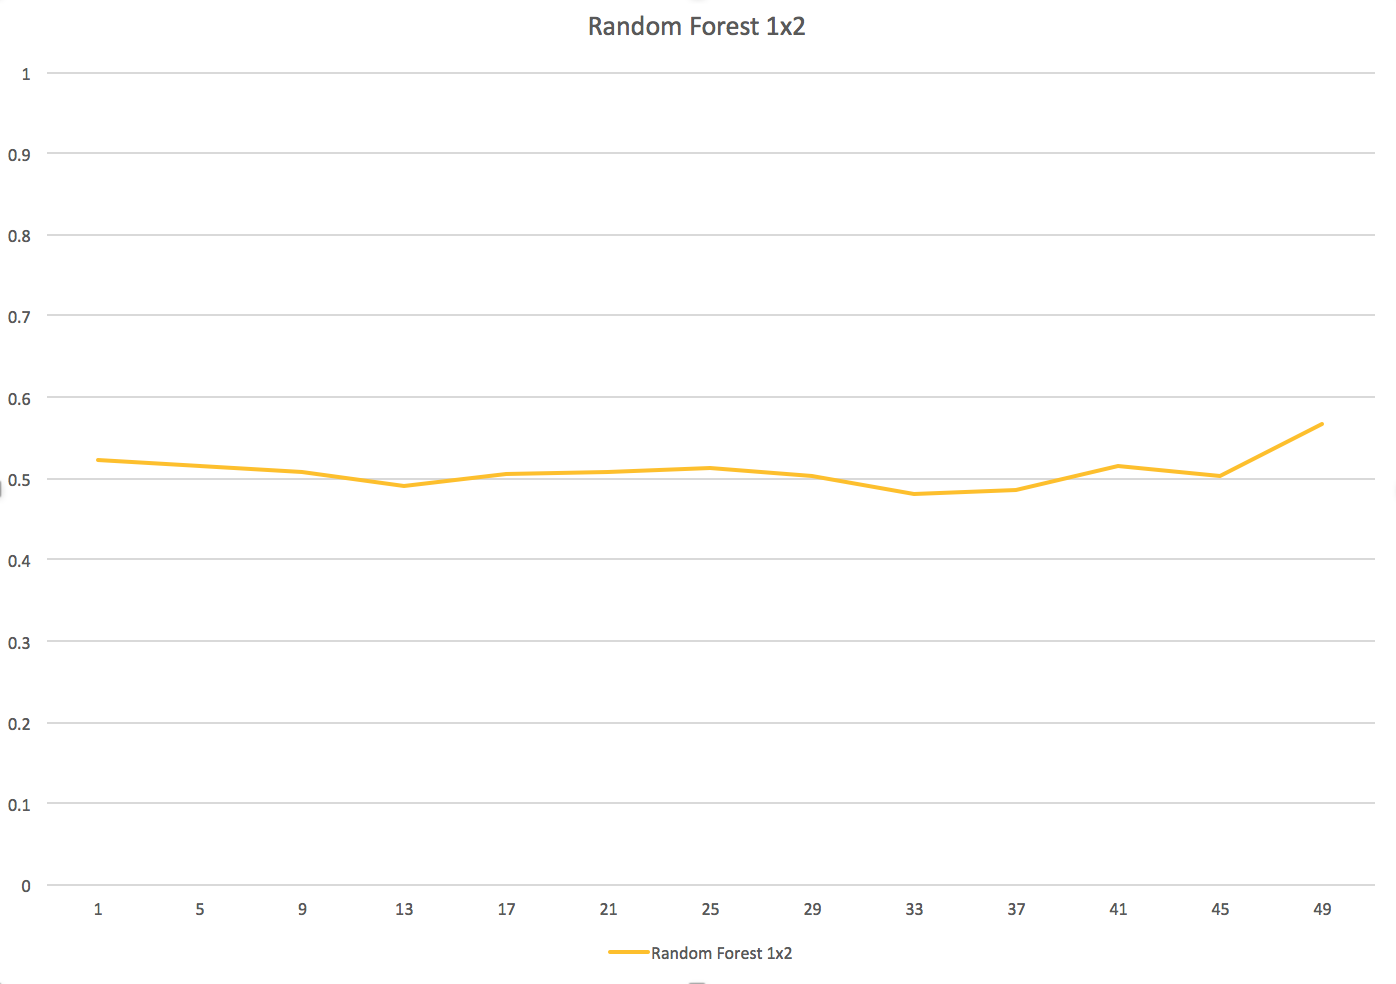
\includegraphics[width=8cm,height=5cm]{images/rf_1x2.png} &   
  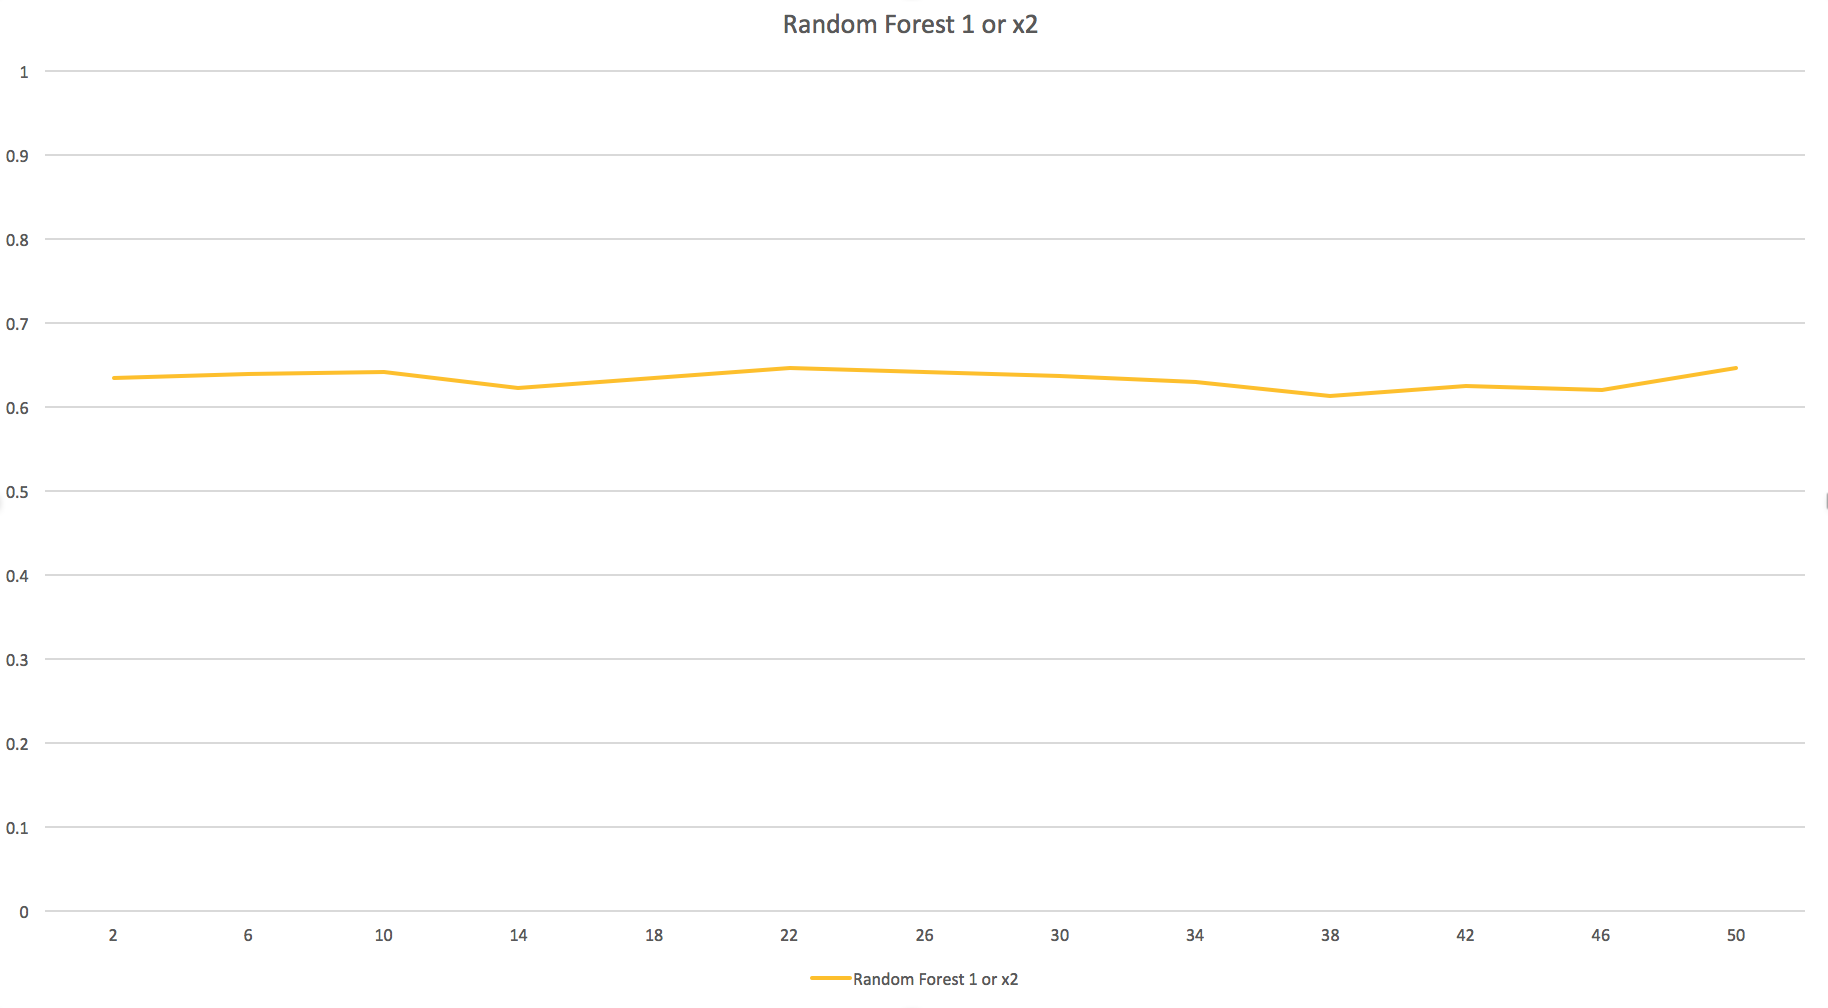
\includegraphics[width=8cm,height=5cm]{images/rf_1_or_x2.png} \\
(а) 1 Х 2 & (б) 1 или Х2 \\
 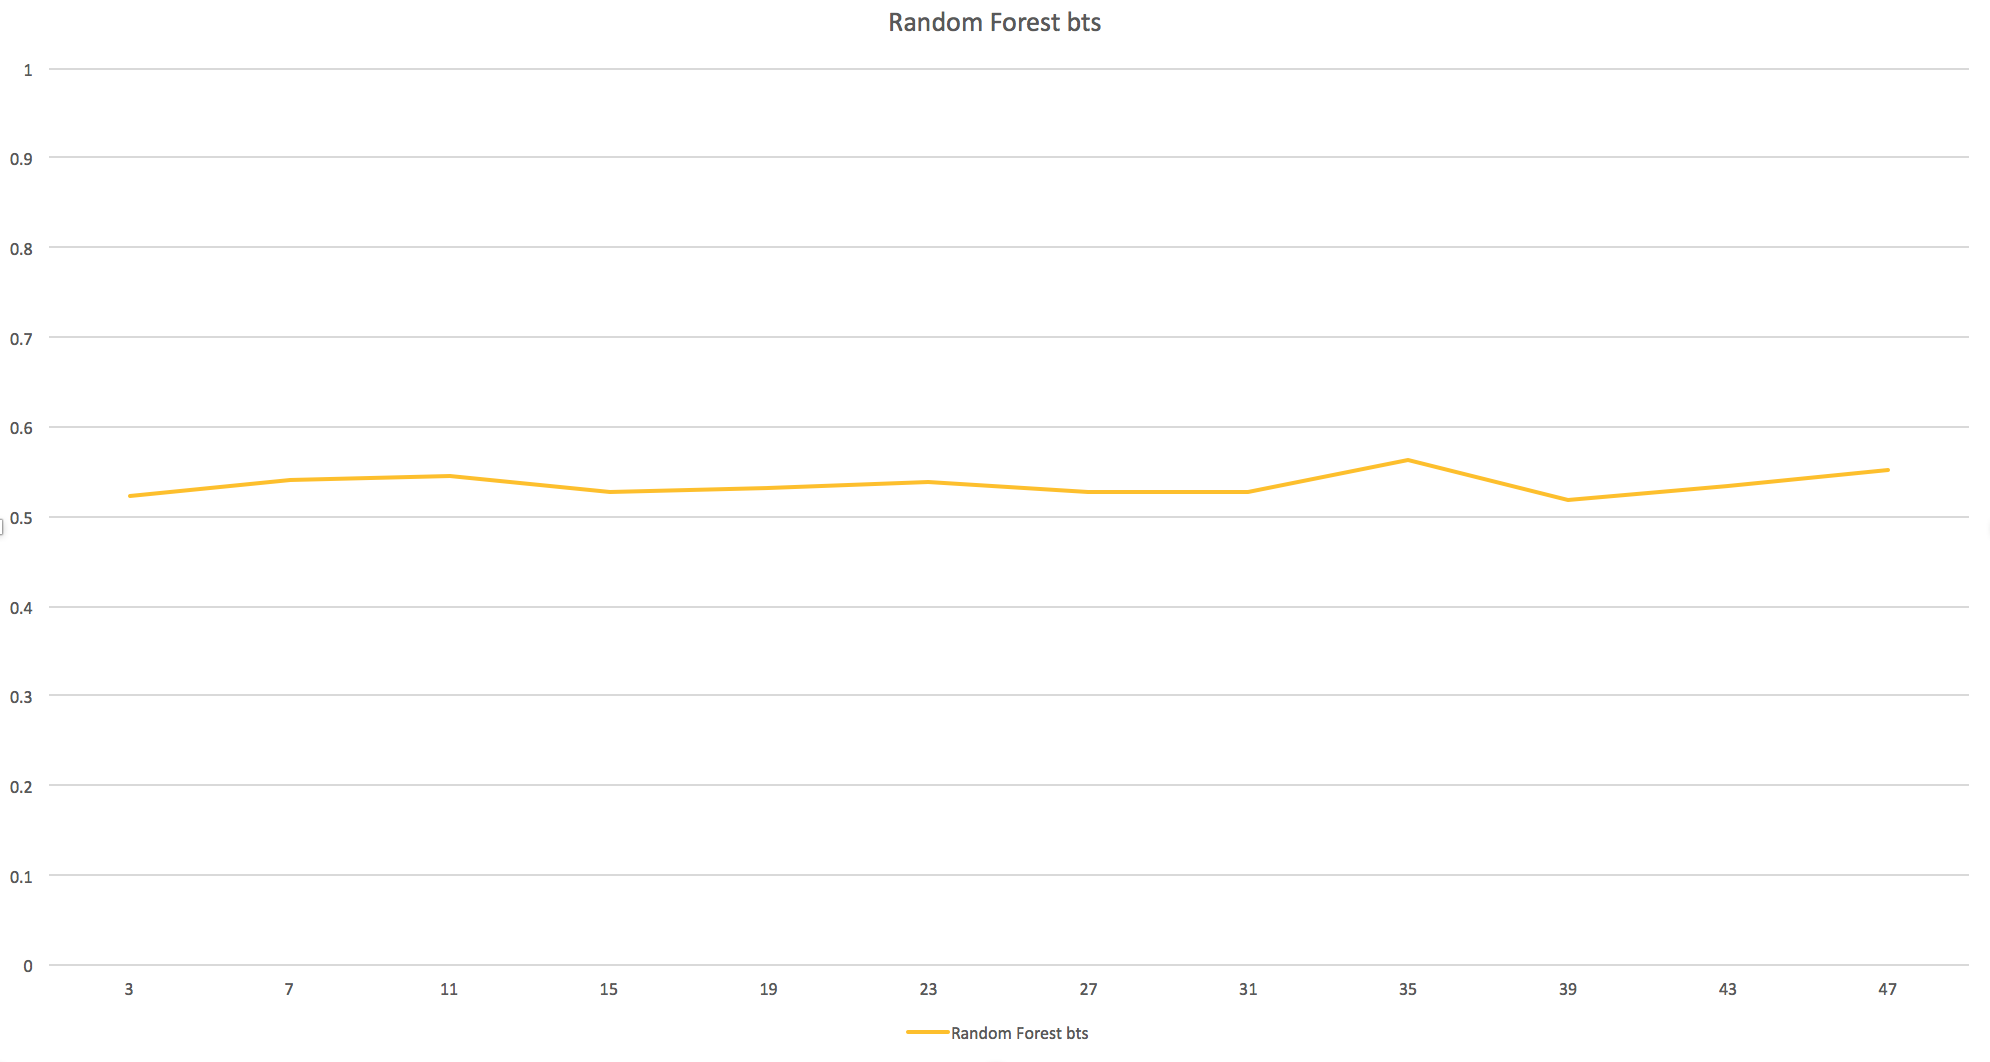
\includegraphics[width=8cm,height=5cm]{images/rf_bts.png}
 &   
 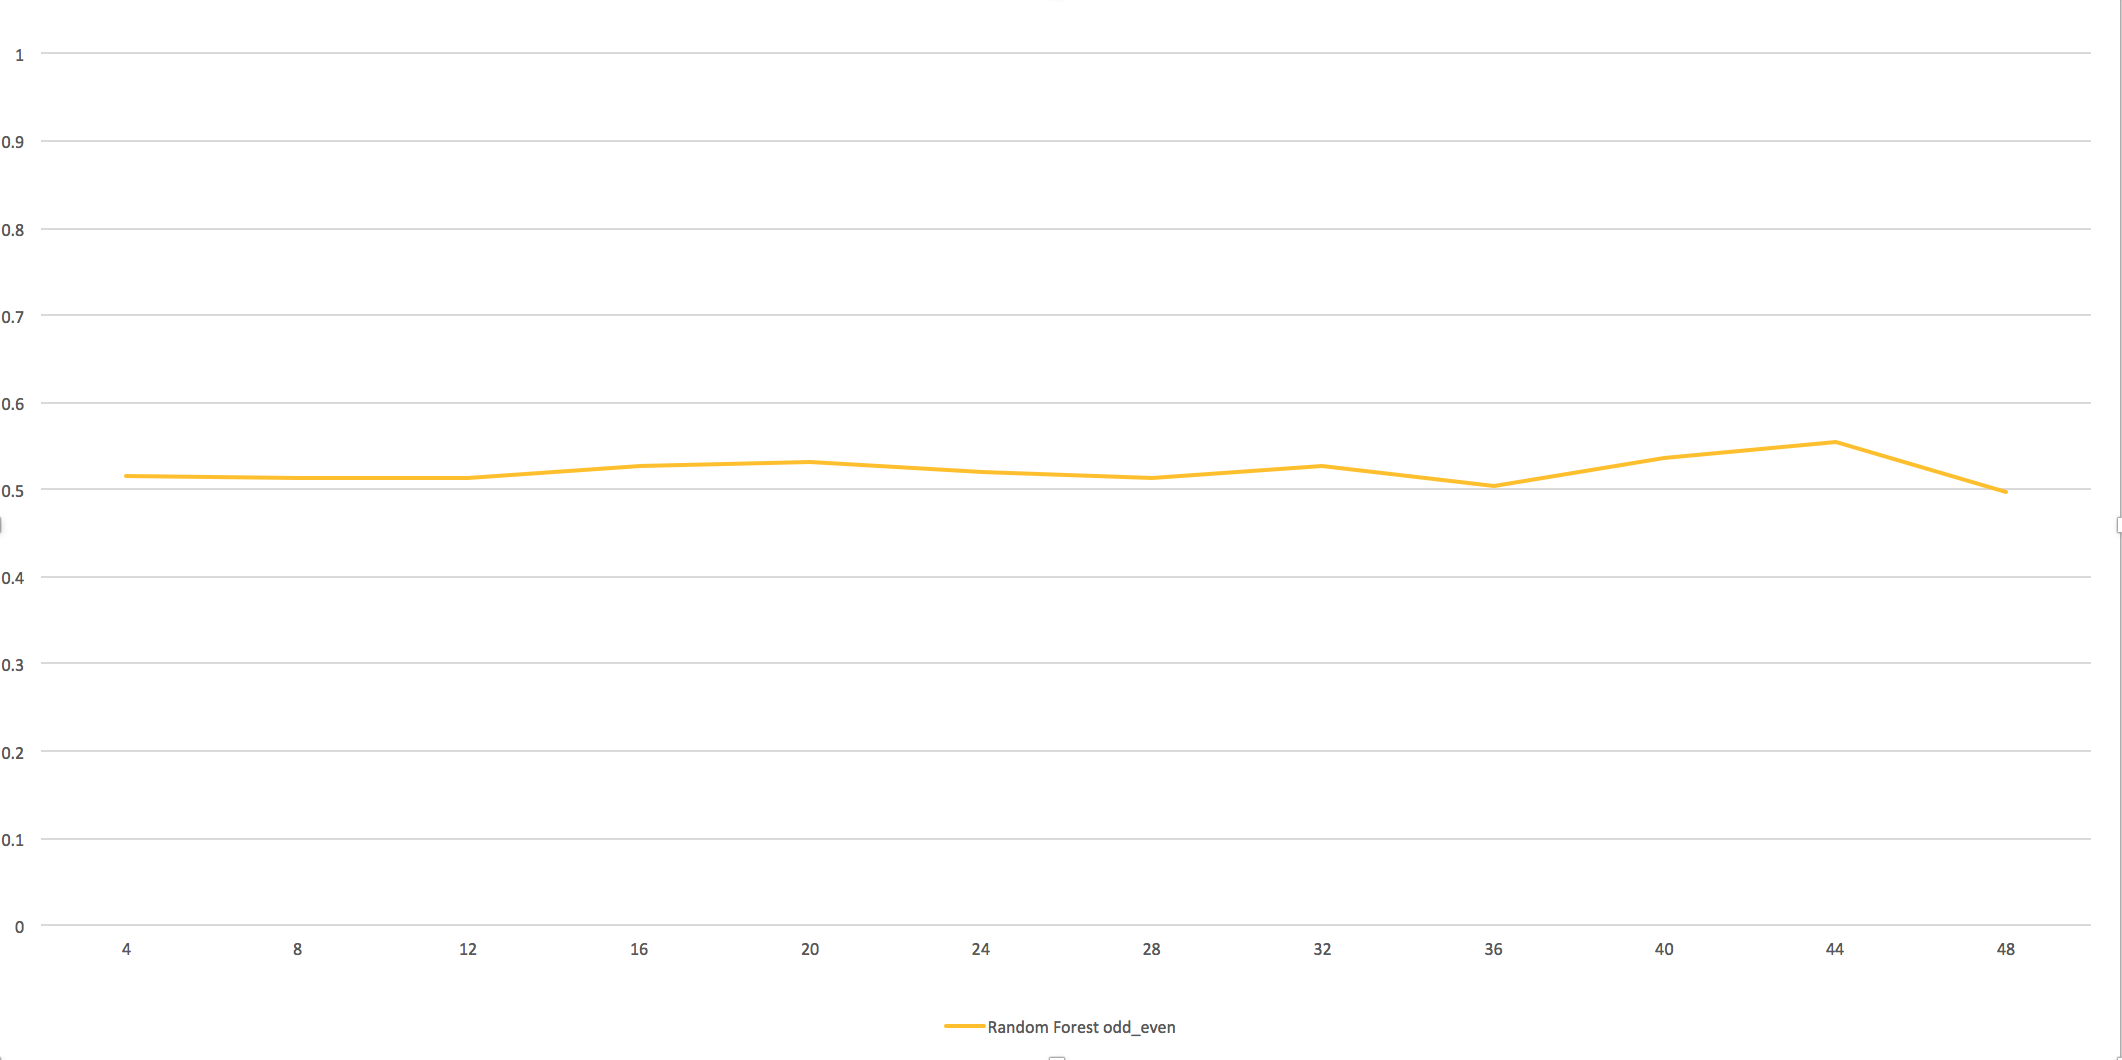
\includegraphics[width=8cm,height=5cm]{images/rf_odd_even.png} \\
(в) дали двата тима ќе поентираат & (г) парен/непарен број на голови \\
\end{tabular}
\caption{Резултати од тестирање со случајни шуми}
\label{fig:random_forest}
\end{figure}

\subsection{Екстремно случаjни дрва}

Во екстремно рандомизирани дрвја \cite{geurts2006extremely}, случајноста оди еден чекор понатаму во начинот на кој се пресметуваат поделбите. Како во случајни шуми, се користи случајно подмножество на карактеристични кандидати, но наместо да се бараат најдискриминирачки прагови, праговите се избираат по случаен избор за секоја кандидатска функција, а најдобриот од овие прагови генерирани по случаен избор се земаат како правило за разделување. Ова обично овозможува малку повеќе да се намали варијансата на моделот, на сметка на малку поголемо зголемување на пристрасноста.

На сликa \ref{fig:ert} се прикажани резултатите од тестирањето на сите податочни множества со екстремно случаjни дрва поделени по класа. Најдобри резултати овој алгоритам постигнува кај множествата 49 и 50 дефинирани во табела \ref{table:datasets}, со 57.7\% за класифицирање на 1 Х 2 игра, односно 66.67\% за класифицирање на 1 или Х2 игра.

\begin{figure}[H]
\centering
\begin{tabular}{cc}
  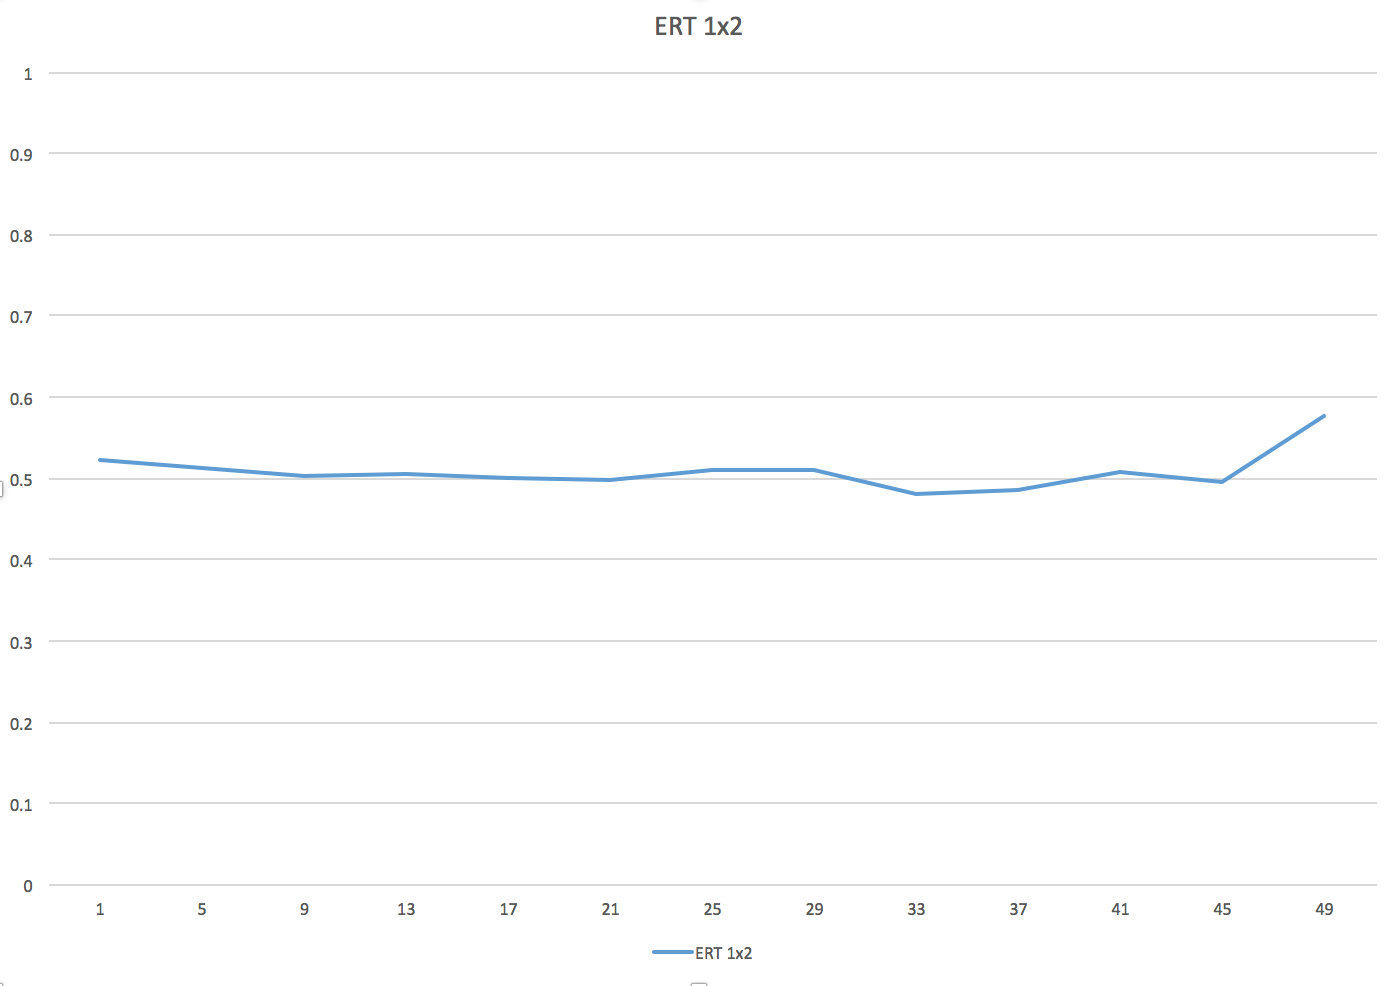
\includegraphics[width=8cm,height=5cm]{images/ert_1x2.png} &   
  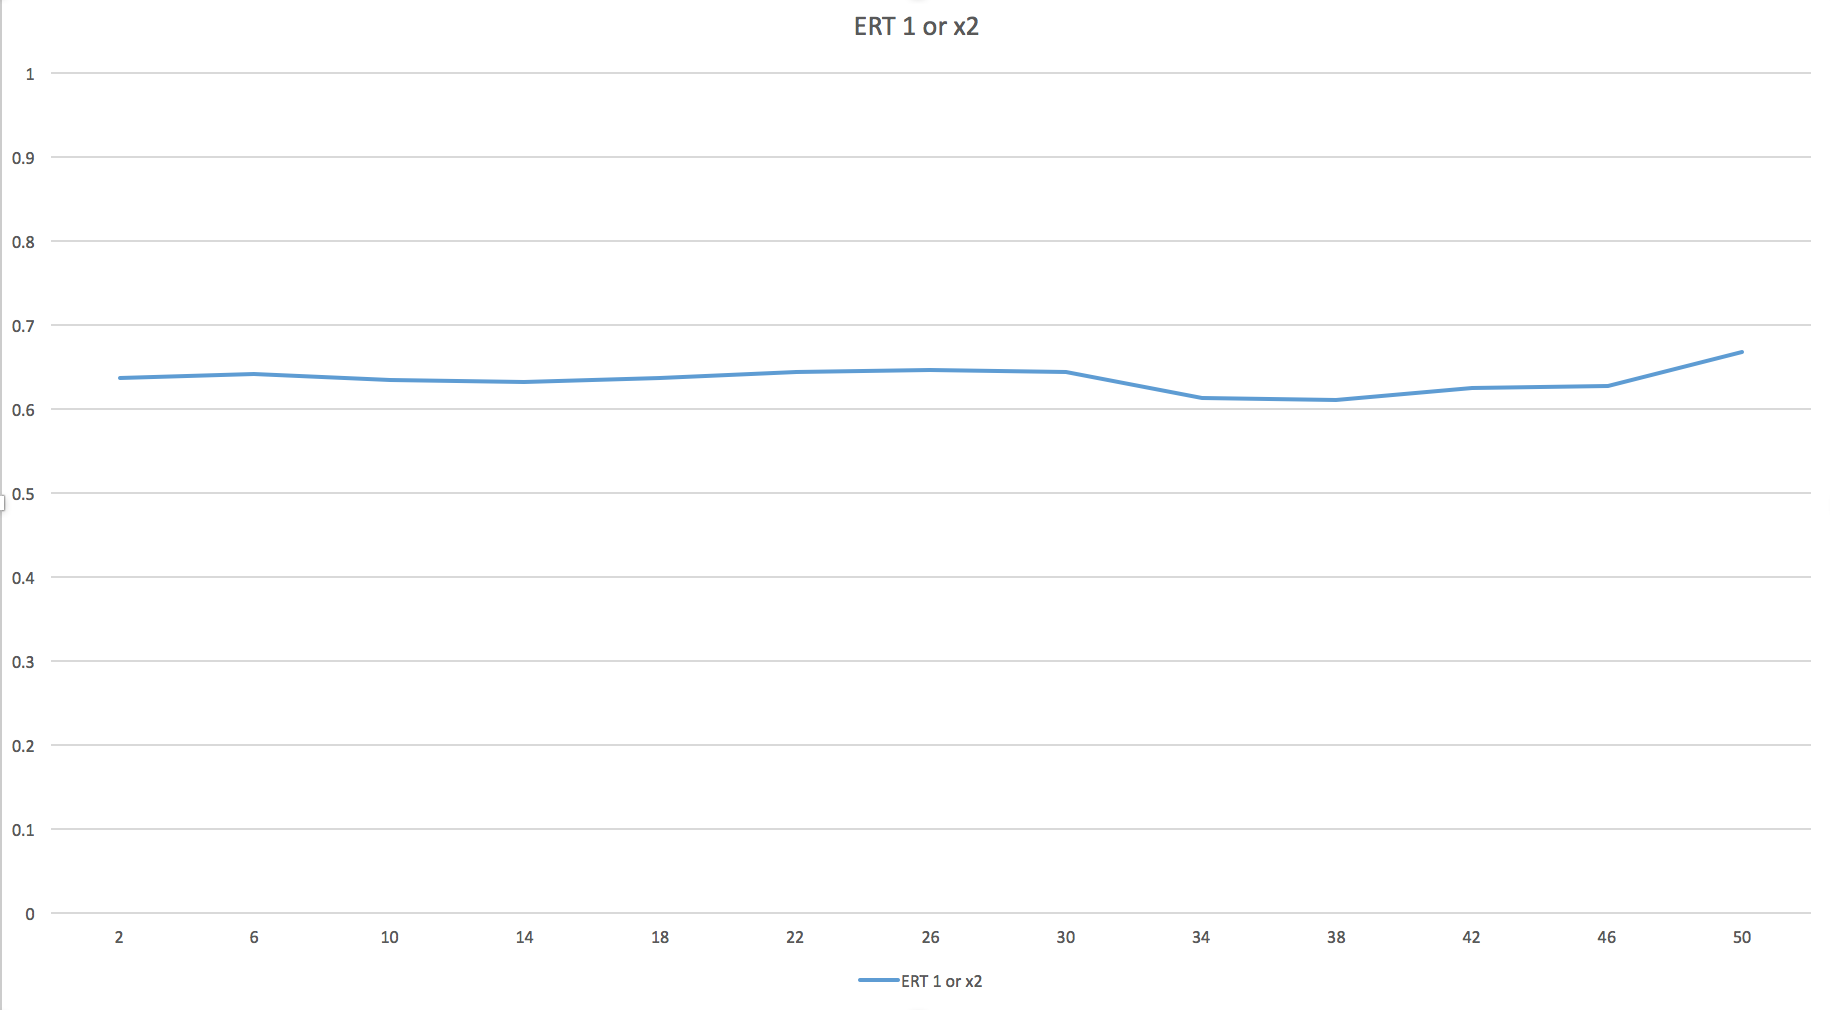
\includegraphics[width=8cm,height=5cm]{images/ert_1_or_x2.png} \\
(а) 1 Х 2 & (б) 1 или Х2 \\
 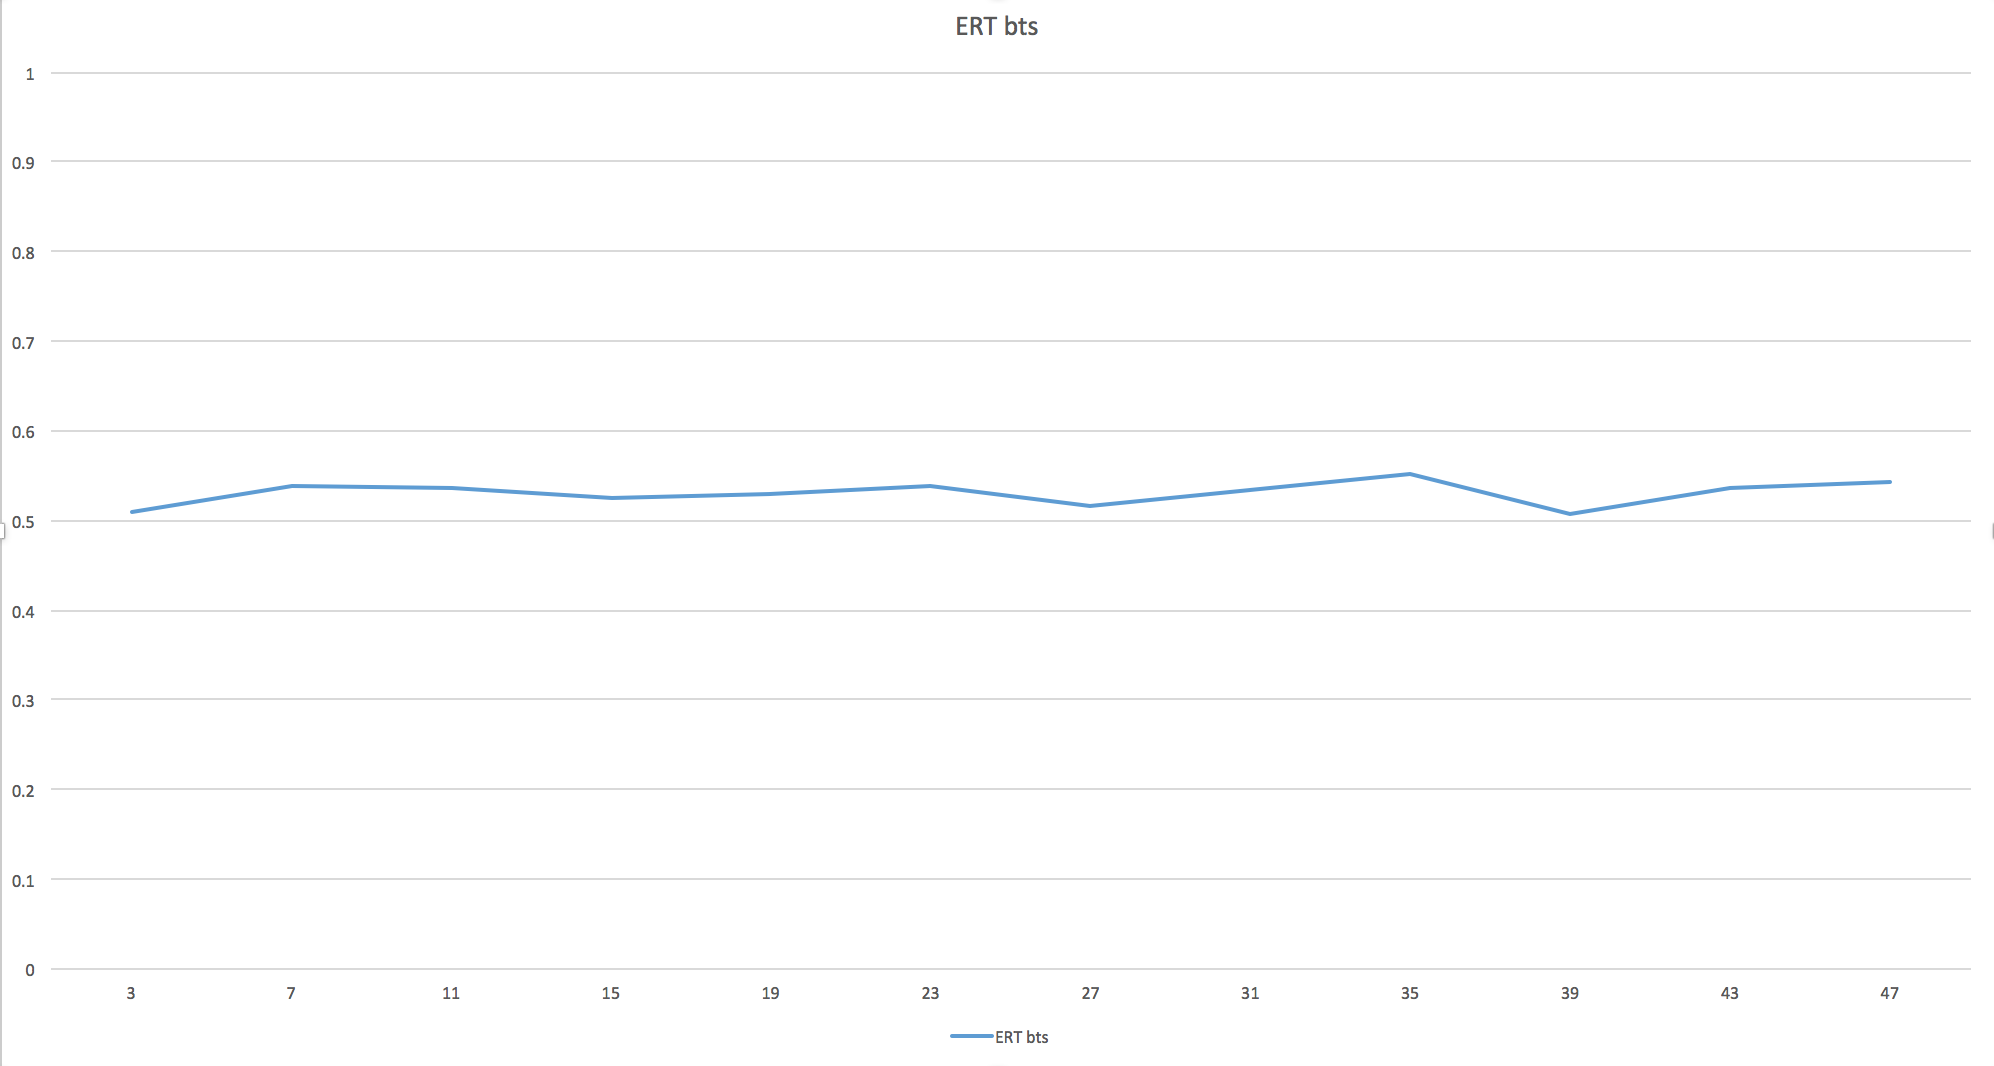
\includegraphics[width=8cm,height=5cm]{images/ert_bts.png}
 &   
 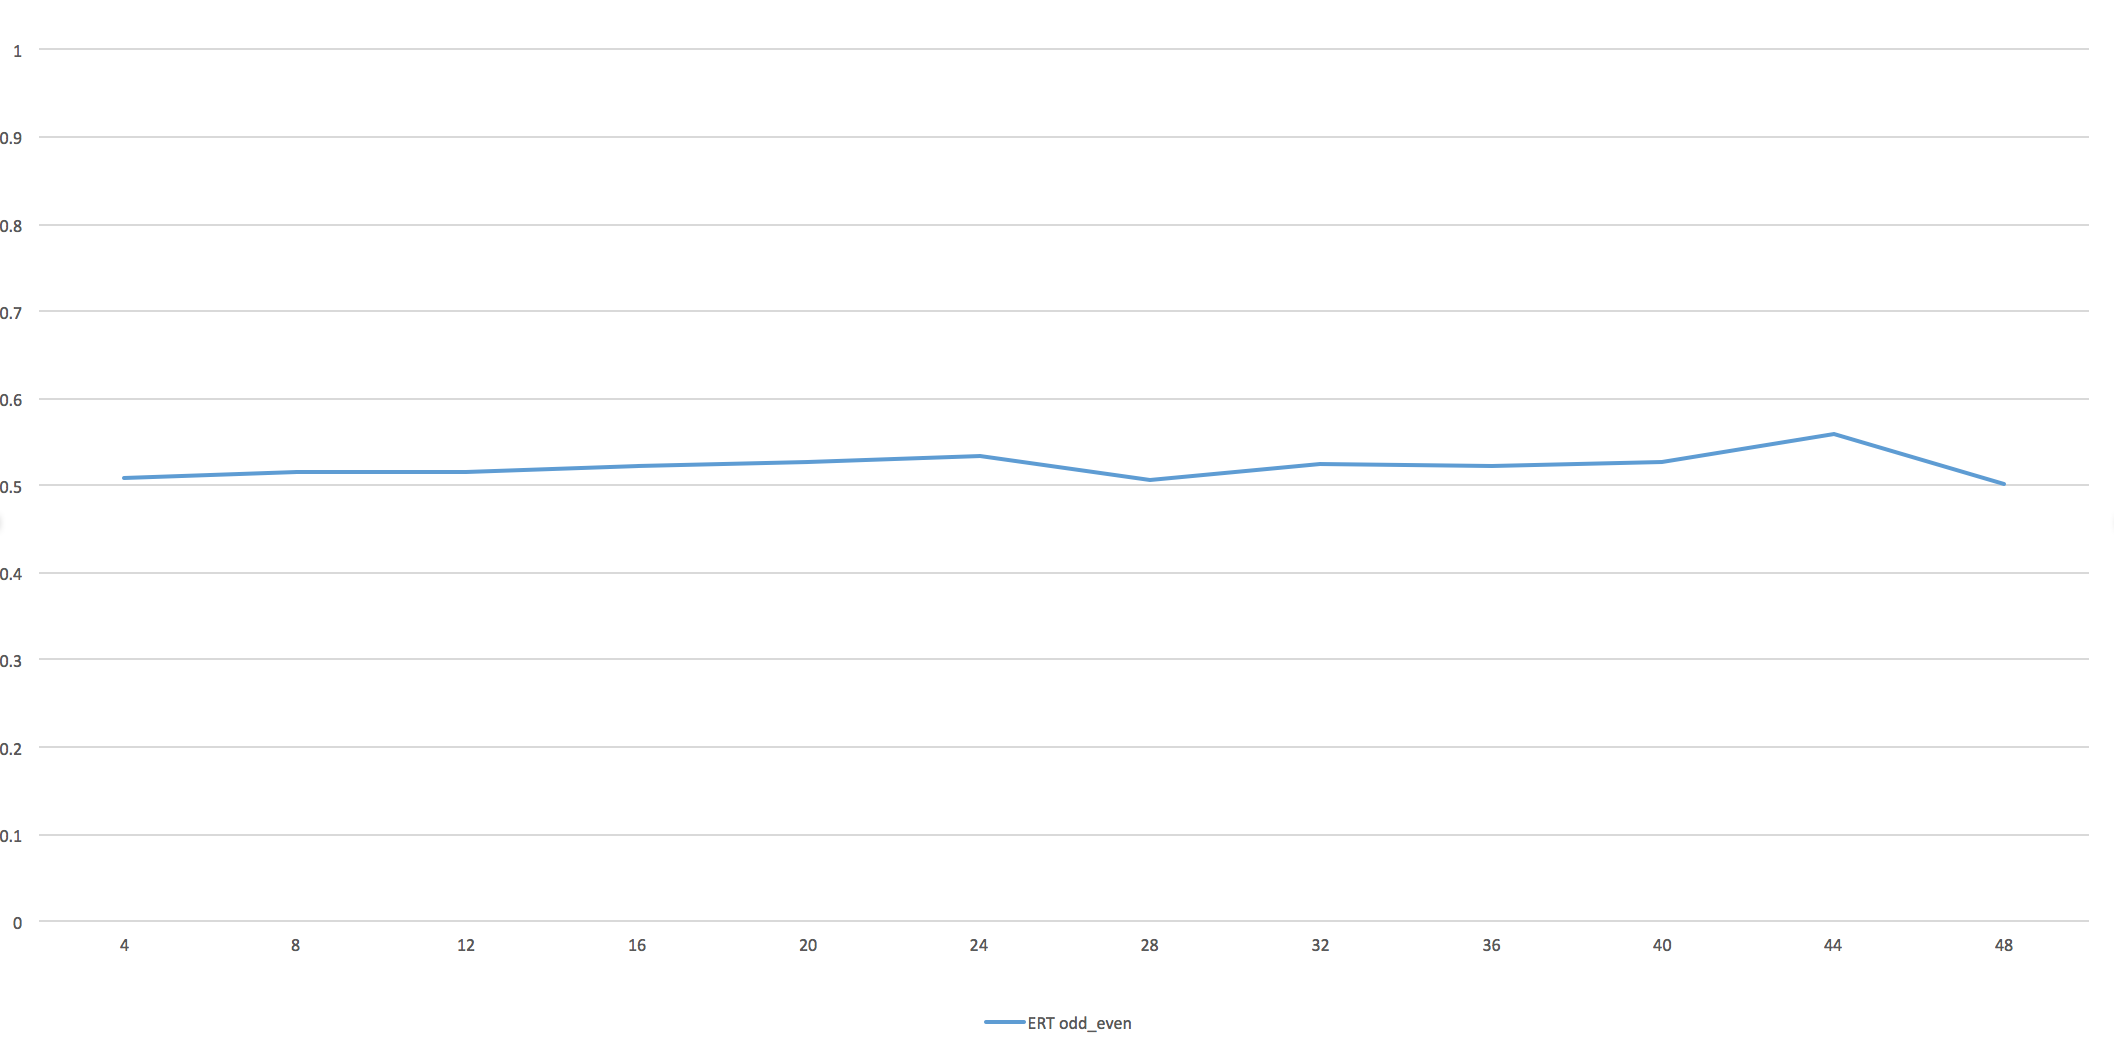
\includegraphics[width=8cm,height=5cm]{images/ert_odd_even.png} \\
(в) дали двата тима ќе поентираат & (г) парен/непарен број на голови \\
\end{tabular}
\caption{Резултати од тестирање со екстремно случаjни дрва}
\label{fig:ert}
\end{figure}


\section{Вештачки невронски мрежи}
Полето на вештачките невронски мрежи \cite{schalkoff1997artificial} честопати се нарекуваат и само невронски мрежи, истражува како едноставни модели на биолошки мозоци може да се искористат за решавање на тешките пресметковни задачи како што се задачите за предвидувачко моделирање што ги гледаме во машинско учење. Целта не е да се создадат реални модели на мозокот, туку да се развијат робустен алгоритми и структури на податоци кои можеме да ги користиме за моделирање на тешки проблеми.
Моќта на невронските мрежи доаѓа од нивната способност да ја научат застапеноста во податоците за обука и како најдобро да се поврзат со излезната променлива што сакаме да ја предвидиме. Во оваа смисла, невронските мрежи учат мапирање. Математички, тие се способни да научат која било функција за мапирање и се докажа дека е универзален апроксимациски алгоритам.
Предвидувачката способност на невронските мрежи доаѓа од хиерархиската или повеќеслојна структура на мрежите. Структурата на податоци може да ги одбере, научи да ги претставува, функциите на различни размери или резолуции и да ги комбинира во функции со повисок редослед. На пример од линии, до збирки на линии до форми.

Основната градежна единка за невронските мрежи се вештачки неврони.
Ова се едноставни пресметковни единици кои имаат пондерирани влезни сигнали и произведуваат излезен сигнал со користење на функцијата за активирање.

Пондерираните влезови се сумираат и пренесуваат преку функцијата за активација, понекогаш наречена функција за трансфер.
Функцијата за активација е едноставно мапирање на сумиран пондериран влез на излезот на невронот. Таа се нарекува функција за активација, бидејќи го регулира прагот на активирање на невронот и сила на излезниот сигнал.
Традиционално се користат нелинеарни функции за активирање. Ова и овозможува на мрежата да ги комбинира влезовите на покомплексни начини и, за возврат, обезбедува побогата можност во функциите што може да ги моделираат. Нелинеарните функции како што е логистичката, исто така наречена сигмоидна функција, се користат за да се изведе вредност помеѓу 0 и 1 со дистрибуција во форма на S (лат.), и хиперболичната тангентна функција, која ја дава истата распределба но во опсегот од -1 до +1 .
Во последно време функцијата за активација на исправувачот е покажана за да обезбеди подобри резултати.

Невроните се наредени во мрежи на неврони.
Редот на невроните се нарекува слој и една мрежа може да има повеќе слоеви. Архитектурата на невроните во мрежата често се нарекува мрежна топологија.

Долниот слој што го зема влезот од вашата група на податоци се нарекува видлив слој, бидејќи е изложениот дел од мрежата. Често, невронската мрежа е нацртана со видлив слој со еден неврон по влезна вредност или колона во вашиот назив на податоци. Овие не се неврони како што е опишано погоре, туку едноставно ја пренесуваат влезната вредност иако на следниот слој.

Слоевите по влезниот слој се нарекуваат скриени слоеви, бидејќи тие не се директно изложени на влезот. Наједноставната мрежна структура е да има еден неврон во скриениот слој кој директно ја дава вредноста.
Со оглед на зголемувањето на компјутерската моќ и ефикасните библиотеки, може да се конструираат многу длабоки невронски мрежи. Длабоко учење може да се однесува на тоа да имате многу скриени слоеви во вашата невронска мрежа. Тие се длабоки, бидејќи тие би биле незамисливо бавно да тренираат историски, но може да потрае неколку секунди или минути ако се обучат со користење на современи техники и хардвер.

Последниот скриен слој се нарекува излезен слој и е одговорен за изнесување на вредност или вектор на вредности кои одговараат на формат потребен за проблемот. 

\subsection{Густо поврзани невронски мрежи}

Од експериментите со претходните алгоритми за машинско учење забележавме дека две податочни множества постојано ни даваа најдобри резултати во однос на останатите. Множествата 49 и 50 дефинирани според табела \ref{table:datasets} всушност ги имаат истите атрибути и истата сегментација, но со различни класи. Во овие две множества се земани само натпреварите од англиската премиер лига и секој тим има одиграно ист број натпревари како останатите тимови во множеството. За таа цел одлучивме да го продолжиме нашето истражување само со овие податочни множества. 

За развојот на моделите на невронските мрежи користевме користевме минималистичка библиотека Керас (Keras анг.) напишана во Python програмскиот јазик и може да работи со помош на Theano или TensorFlow. Во Керас постојат повеќе имплементации на невронски мрежи како што се рекурентни невронски мрежи или конволуциски невронски мрежи, но во нашиот случај ние користиме густо поврзани невронски мрежи или целосно поврзани невронски мрежи. Архитектурата на густо поврзаните невронски мрежи е направена така што секој јазол од претходниот слој е поврзан со секој јазол од следниот слој. Проблемот кој го решаваме е претставен како функциско мапирање и овој тип на архитектура е соодветен за вакви проблеми.

Причината зашто невронските мрежи се толку тешки да се конфигурираат е бидејќи постојат многу параметри кои треба да се постават. Во нашиот случај за наѓање на соодветните параметри, применивме техники на пребарување како во \cite{lameski2015svm}. Во табела \ref{table:params} се прикажани параметрите за кои пребарувавме и нивниот опис. 

\begin{table}[hbtp]
 \centering
 \scalebox{0.45}{%
 \begin{tabular}{| c | c |}
 \hline
 параметар & опис \\ 
 \hline
 \hline
 batch\_size & бројот на инстанци кои се оценуваат пред да се изврши ажурирање на тежината во мрежата \\ 
 \hline
 epochs & број на итерации во еден тренинг процес \\ 
 \hline
 dropout & случајно поставување фракција на влезни единици на 0 во секое ажурирање за време на обуката, што помага да се спречи претренирање (overfitting, анг.) \\ 
 \hline
 kernel\_constraint & функцијата за ограничување се применува на матрицата на тежини \\ 
 \hline
 neurons & број на неврони во скриениот слој \\ 
 \hline
  activation & активациска функција \\ 
 \hline
 optimizer & оптимизациски алгоритам \\ 
 \hline
 loss & вредност што ние се обидуваме да ја минимизираме за време на нашата обука на моделот \\ 
 \hline
\end{tabular}}
\caption{Параметри за конфигурација на модел на невронски мрежи во Керас}
\label{table:params}
\end{table}
За скриените слоеви ја користевме 'relu' (rectified linear unit) активациската функција како параметар за активација, додека во излезниот слој користевме сигмоидна функција 'sigmoid'. 
Ја користиме сигмоидната функција на излезниот слој за да осигуриме дека нашата излезна мрежа е помеѓу 0 и 1 и лесно може да се мапира или на веројатност од 0 до 1 или припрема на класификација на било која класа со стандарден праг од 0,5. Како оптимизациски алгоритам го користиме 'adam' \cite{kingma2014adam}. За 'loss' параметарот како вредности кои треба да ги минимизираме за множеството 49 користевме 'categorical\_crossentropy' бидејќи овде имаме 3 класи (1 Х 2) и излезниот слој ќе содржи 3 неврони, додека за множеството 50 користевме 'binary\_crossentropy' бидејќи во ова множество се само 2 класи (1 или Х2) и излезниот слој може да се претстави само со 1 неврон. Oстанатите параметри ги добивме со пребарување и оптимизација.

\begin{table}[hbtp]
 \centering
 \scalebox{0.7}{%
 \begin{tabular}{| c | c |}
 \hline
 параметар & вредности \\ 
 \hline
 \hline
 batch\_size & 20, 32, 64\\ 
 \hline
 epochs & 50, 80, 120 \\ 
 \hline
 dropout & 0.2, 0.5, 0.8 \\ 
 \hline
 kernel\_constraint & 4, 6, 8 \\ 
 \hline
 hidden\_layers & 1, 2, 3, 4 \\
  \hline
 neurons &  (влезна димезнија)/4, (влезна димензија)/2, (влезна димензија)*1, (влезна димензија)*2 \\ 
 \hline
\end{tabular}}
\caption{Вредности на хипер-параметрите користени за пребарување и оптимизација на моделот}
\label{table:params_grid}
\end{table}

Пребарувањето на параметрите го вршевме со тренирање на тренинг множеството и тестиравме врз валидациското множество. По извршеното пребарување низ вредностите на параметрите прикажани во табела \ref{table:params_grid}, добивме оптимална конфигурација на моделот со параметри прикажани во табела \ref{table:params_conf_49} и табела  \ref{table:params_conf_50}. Резултатите од пребарувањето се прикажани на слика \ref{fig:grid_search_49} и слика  \ref{fig:grid_search_50}.

\begin{figure}[hbtp]
\centering
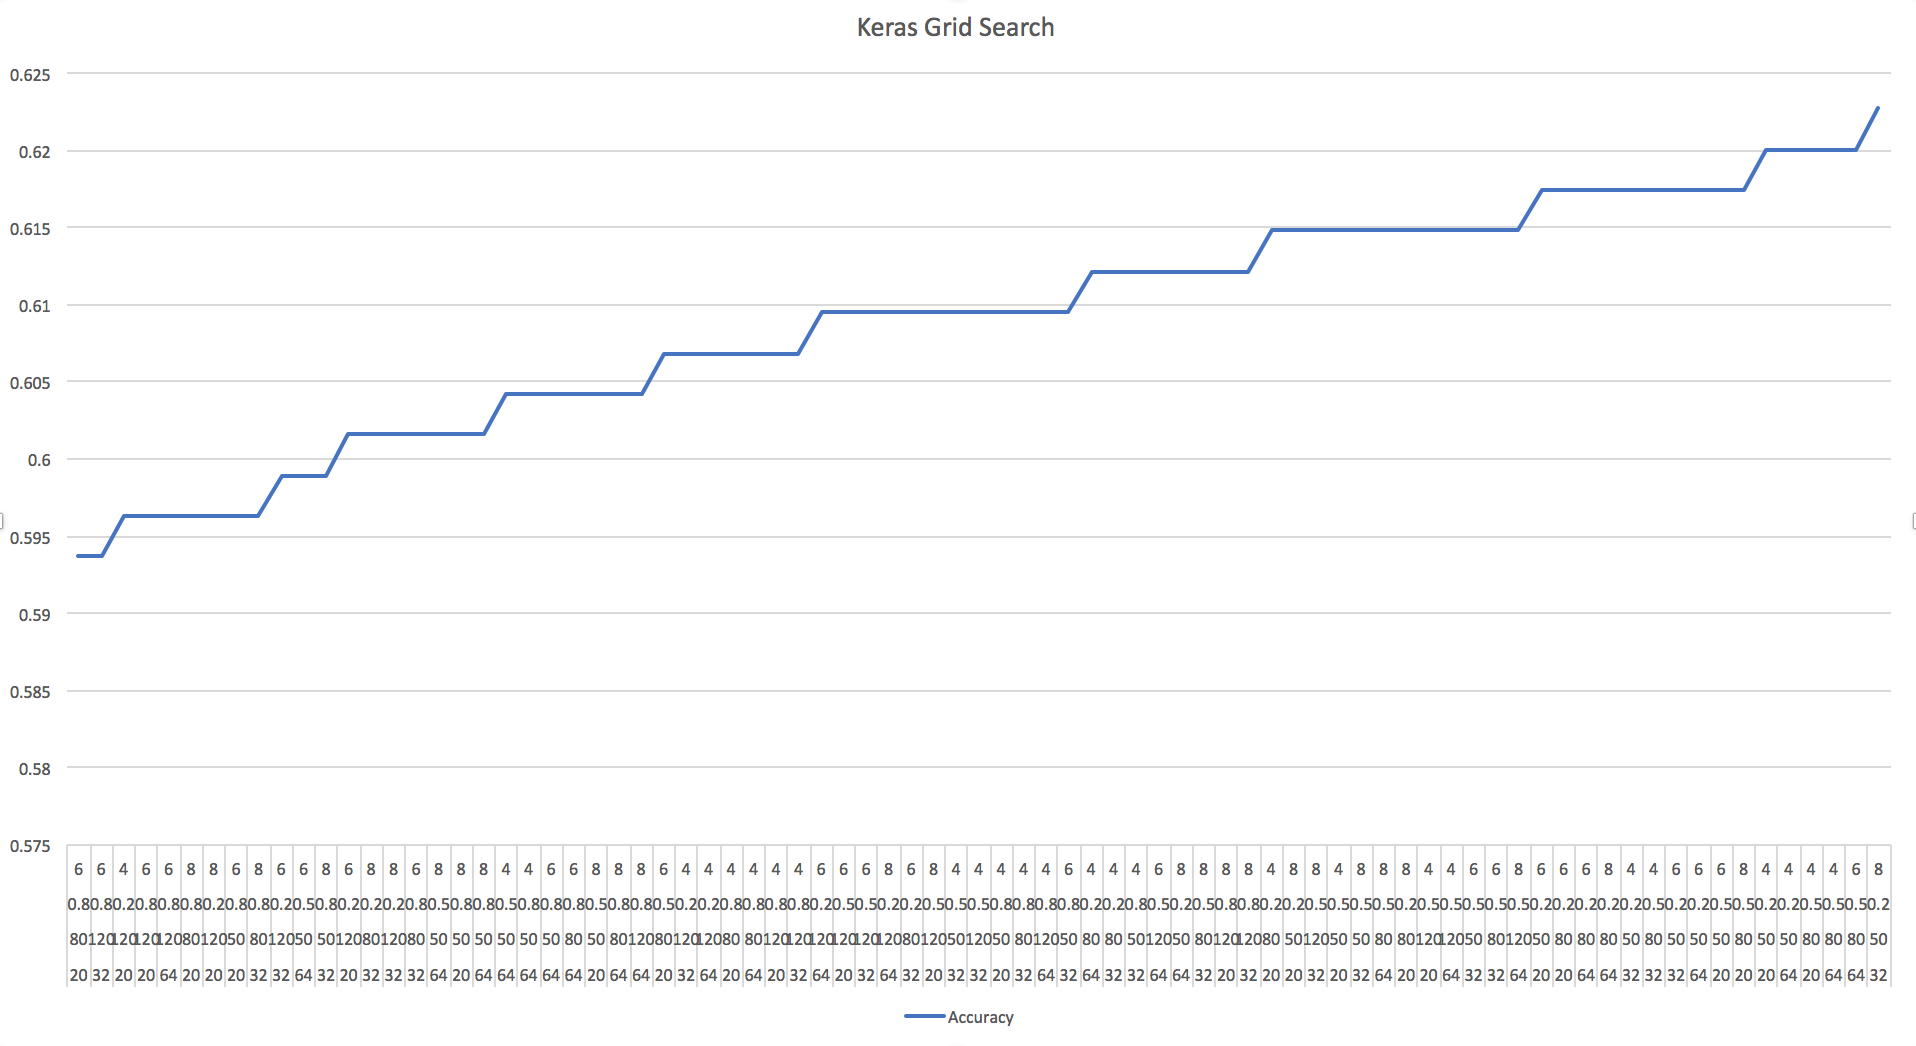
\includegraphics[width=14cm,height=8cm]{images/keras_grid_search.png}
\caption{Оптимизација на моделот преку пребарување за множество 49}
\label{fig:grid_search_49}
\centering
\end{figure}

\begin{figure}[hbtp]
\centering
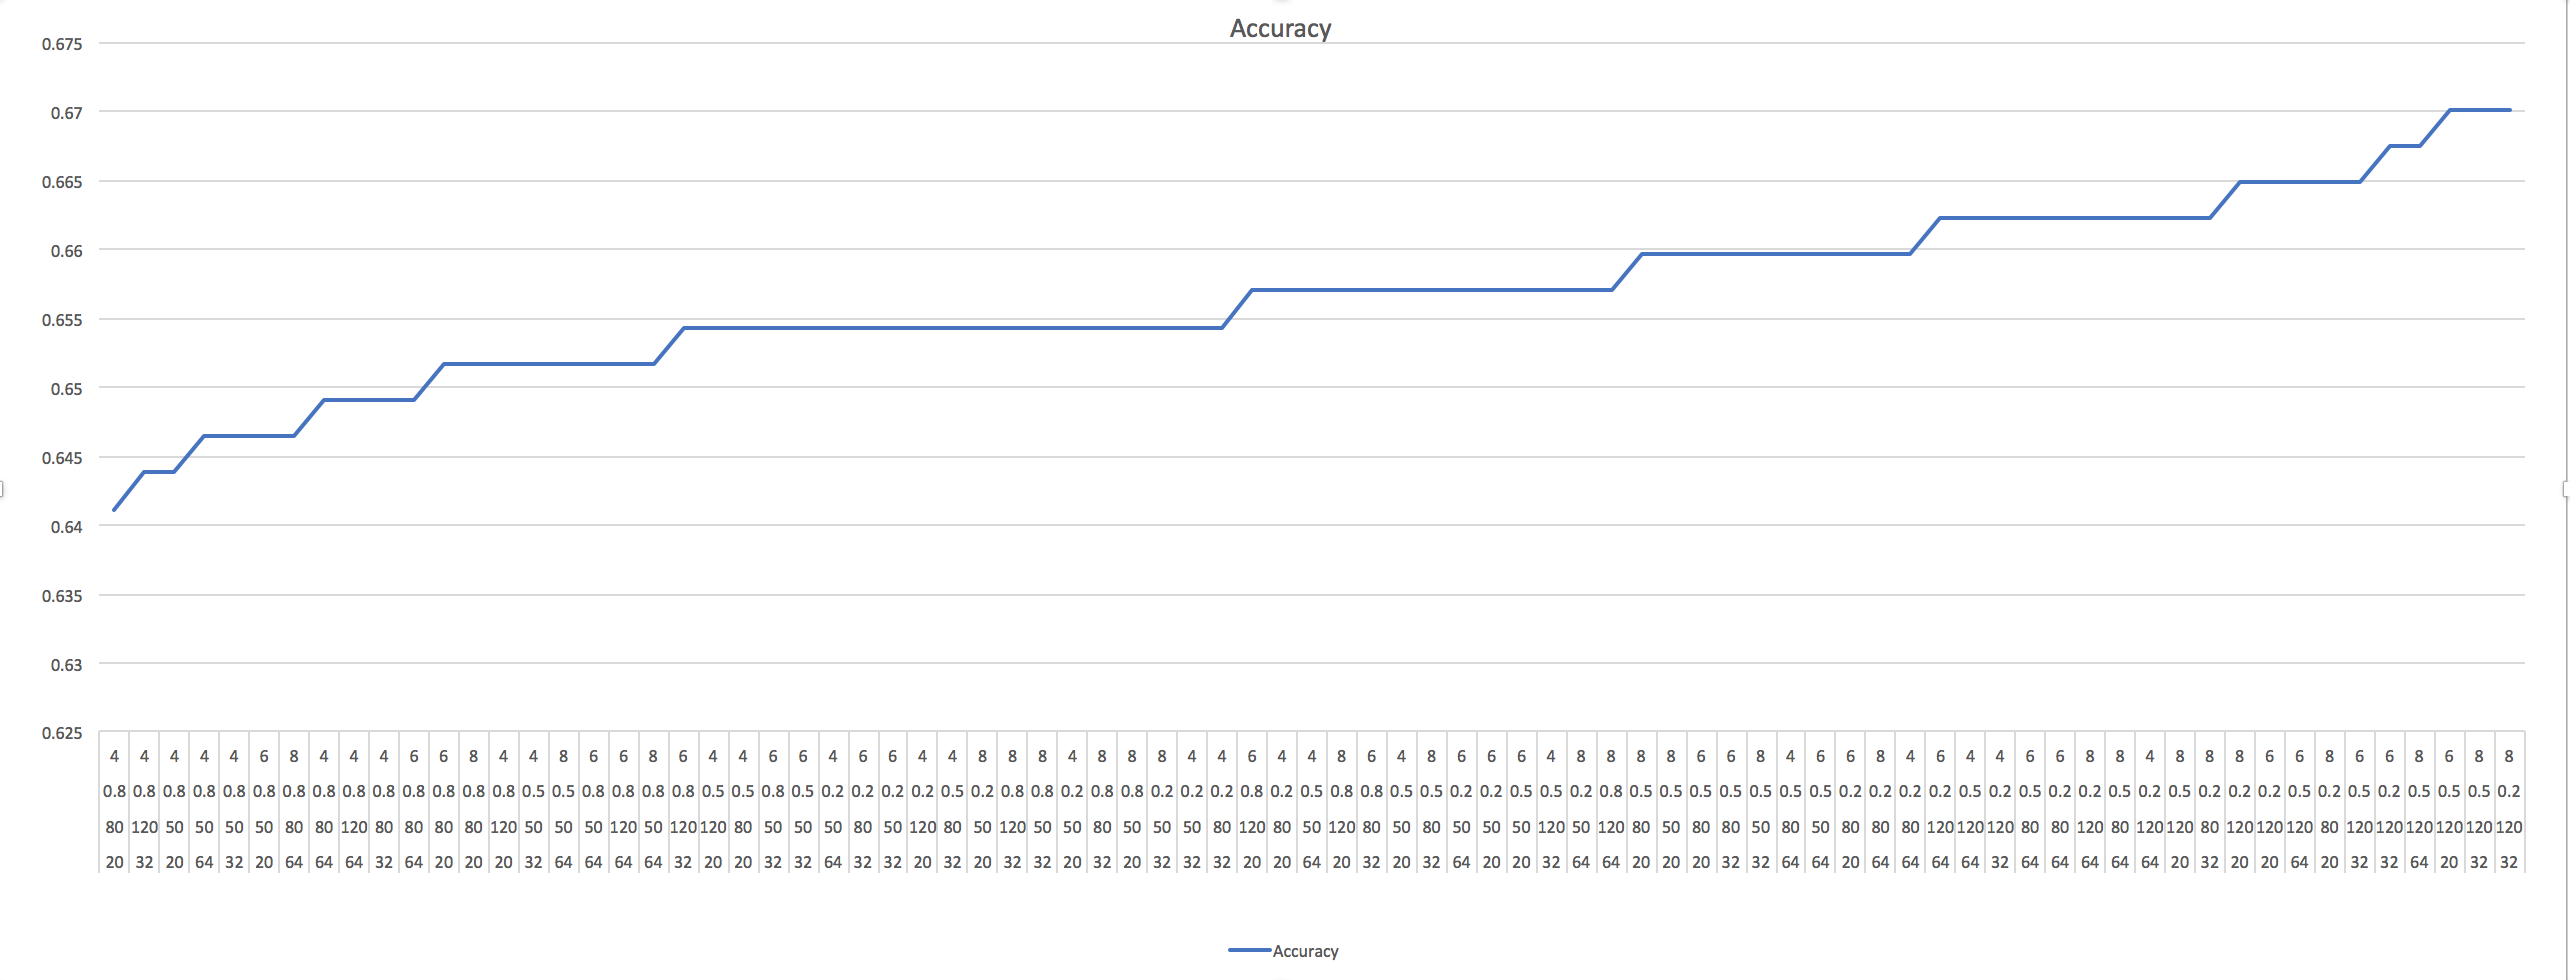
\includegraphics[width=14cm,height=8cm]{images/keras_grid_search_50.png}
\caption{Оптимизација на моделот преку пребарување за множество 50}
\label{fig:grid_search_50}
\centering
\end{figure}

\begin{table}[hbtp]
 \centering
 \scalebox{0.8}{%
 \begin{tabular}{| c | c |}
 \hline
 параметар & вредности \\ 
 \hline
 \hline
 batch\_size & 32\\ 
 \hline
 epochs & 50 \\ 
 \hline
 dropout & 0.2 \\ 
 \hline
 kernel\_constraint &  8 \\ 
 \hline
 hidden\_layers & 1 \\
  \hline
 neurons &  (влезна димезнија)*1 \\ 
 \hline
  activation & 'relu' за скриените слоеви, 'sigmoid' за излезниот слој \\ 
 \hline
 optimizer & 'adam' \\ 
 \hline
 loss & 'categorical\_crossentropy' \\ 
 \hline
\end{tabular}}
\caption{Оптимална конфигурација на моделот во Керас за податочно множество 49}
\label{table:params_conf_49}
\end{table}

\begin{table}[hbtp]
 \centering
 \scalebox{0.8}{%
 \begin{tabular}{| c | c |}
 \hline
 параметар & вредности \\ 
 \hline
 \hline
 batch\_size & 32\\ 
 \hline
 epochs & 120 \\ 
 \hline
 dropout & 0.5 \\ 
 \hline
 kernel\_constraint &  8 \\ 
 \hline
 hidden\_layers & 1 \\
  \hline
 neurons &  (влезна димезнија)*1 \\ 
 \hline
  activation & 'relu' за скриените слоеви, 'sigmoid' за излезниот слој \\ 
 \hline
 optimizer & 'adam' \\ 
 \hline
 loss & 'binary\_crossentropy'\\ 
 \hline
\end{tabular}}
\caption{Оптимална конфигурација на моделот во Керас за податочно множество 50}
\label{table:params_conf_50}
\end{table}

Во следниот чекор на тестирање ги користевме тренинг и валидациското множества како едно целосно тренинг множество и го евалуиравме моделот врз тест множеството. На сличен начин како и пребарувањето на вредностите на параметрите направивме пребарување со цел да најдеме најдобра архитектура на невронска мрежа за нашиот проблем. Пребарувавме низ бројот на неврони и вкупниот број на скриени слоеви. За двете податочни множества добивме најоптимална архитектура со еден скриен слој со ист број на неврони колку и влезниот слој. За множеството 49 добивме архитектура со 26 неврони во влезниот слој, 26 неврони во скриениот слој и 3 во излезниот прикажана на слика . За множеството 50 добивме архитектура со 18 неврони во влезниот слој, 18 неврони во скриениот слој и 1 во излезниот прикажана на слика . При нормализација на податоците најдобри резултати ни даде min-max во опсег од 0 до 1, додека пак при кодирањето ги пробавме бинарното и класното кодирање, каде класното кодирање постигна подобри резултати. 
За множеството 49 добивме точност од 55.91\% додека за множеството 50 добивме точност од 67.38\%.

\begin{figure}[H]
\centering
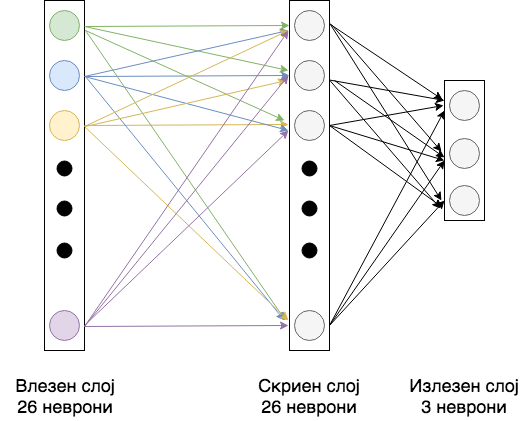
\includegraphics[scale=0.34]{images/Neural_net_49.png}
\caption{Архитектура на невронска мрежа за податочно множество 49}
\label{fig:architecture_49}
\centering
\end{figure}

\begin{figure}[H]
\centering
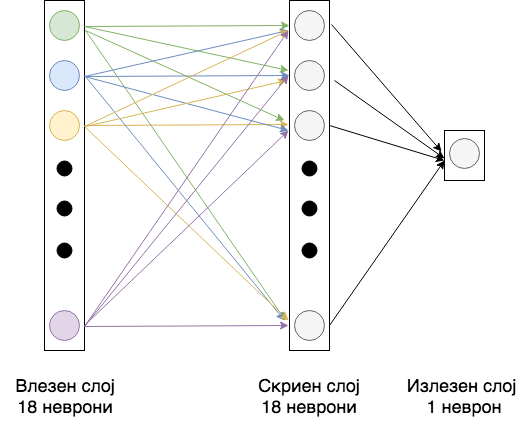
\includegraphics[scale=0.34]{images/Neural_net_50.png}
\caption{Архитектура на невронска мрежа за податочно множество 50}
\label{fig:architecture_50}
\centering
\end{figure}


\chapter{Евалуација на моделите}
\label{sec:evaluation}
Евалуација на моделите ни го одговара прашањето - Како да го одбереме најдобриот модел? Без разлика дали одбираме помеѓу различни алгоритми или ги одбираме оптималните параметри или одбираме помеѓу различни атрибути, нас ни треба процедура за евалуација на модели за да ни помогне да процениме колку добро еден модел ќе се генерализира на податоците што не бил трениран. Како и да е нам ни требаат и евалуациски метрики за да ги споредиме со нашите процедури за да можеме да ги квантифицираме перформансите на моделот.

Секогаш ни треба евалуациска метрика што ќе оди заедно со одбрана процедура и изборот на метрика зависи од типот на проблемот кој го решаваме. За регресивни проблеми користиме средна апсолутна грешка или средна квадратна грешка, додека за класификациски проблеми како нашиот досега користевме само класификациска точност. Постојат и други важни метрики кои ќе ги разгледаме во ова поглавје. 
\section{Класификациска точност}
Пред да ги проучиме другите евалуациски метрики, да ја разгледаме прво класификациската точност. За да ја добиеме класификациската точност ние во претходното поглавје го разделивме на тренинг, валидациско и тест множество. Со тренинг и валидациското множество ги наоѓавме најдобрите параметри за нашите модели каде како вредност што треба да ја максимизираме ја земавме точноста. Со тренинг и валидациското множество заедно го трениравме моделот и ги евалуиравме нашите резултати врз тест множеството исто така со точноста. Класификациската точност е всушност процентот на точните предвидувања. На слика \ref{fig:comparison_49} и слика \ref{fig:comparison_50} може да се видат точностите на сите алгоритми за соодветните податочни множества. Од резултатите можеме да забележиме дека за податочното множество 49 каде имаме 3 класи, моделите на екстремно случајни дрва и случајна шума ни даваат подобри резултати, веднаш по нив е моделот добиен со невронската мрежа. Кај множеството 50 каде имаме 2 класи, подобри резултати добиваме кај наивен баесов класификатор, логистичката регресија и машини со носечки вектори, но и моделот на невронските мрежи пак постигна добри резултати. Со ова можеме да заклучиме дека невронските мрежи и во двата случаи се добри предвидувачи.

\begin{figure}[H]
\centering
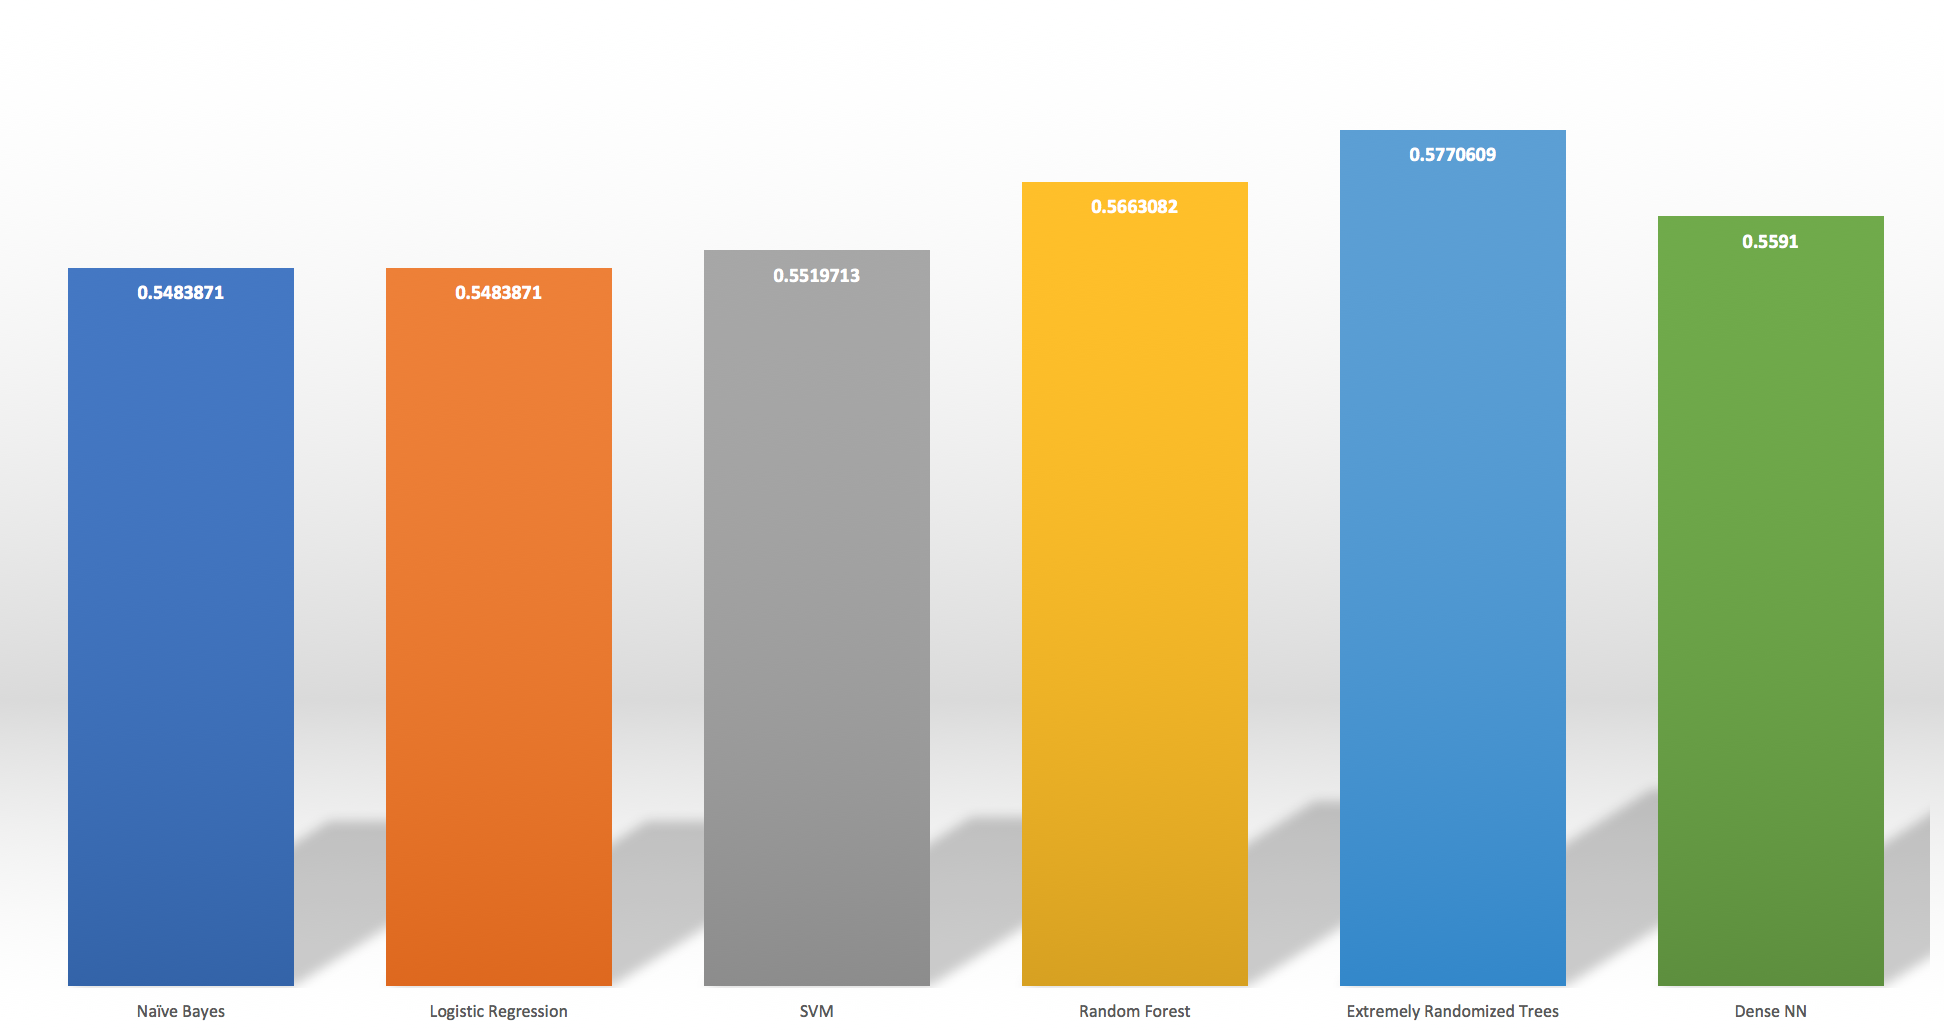
\includegraphics[scale=0.34]{images/comparison_algo_49.png}
\caption{Споредба на резултати од тестирање за податочно множество 49}
\label{fig:comparison_49}
\centering
\end{figure}

\begin{figure}[H]
\centering
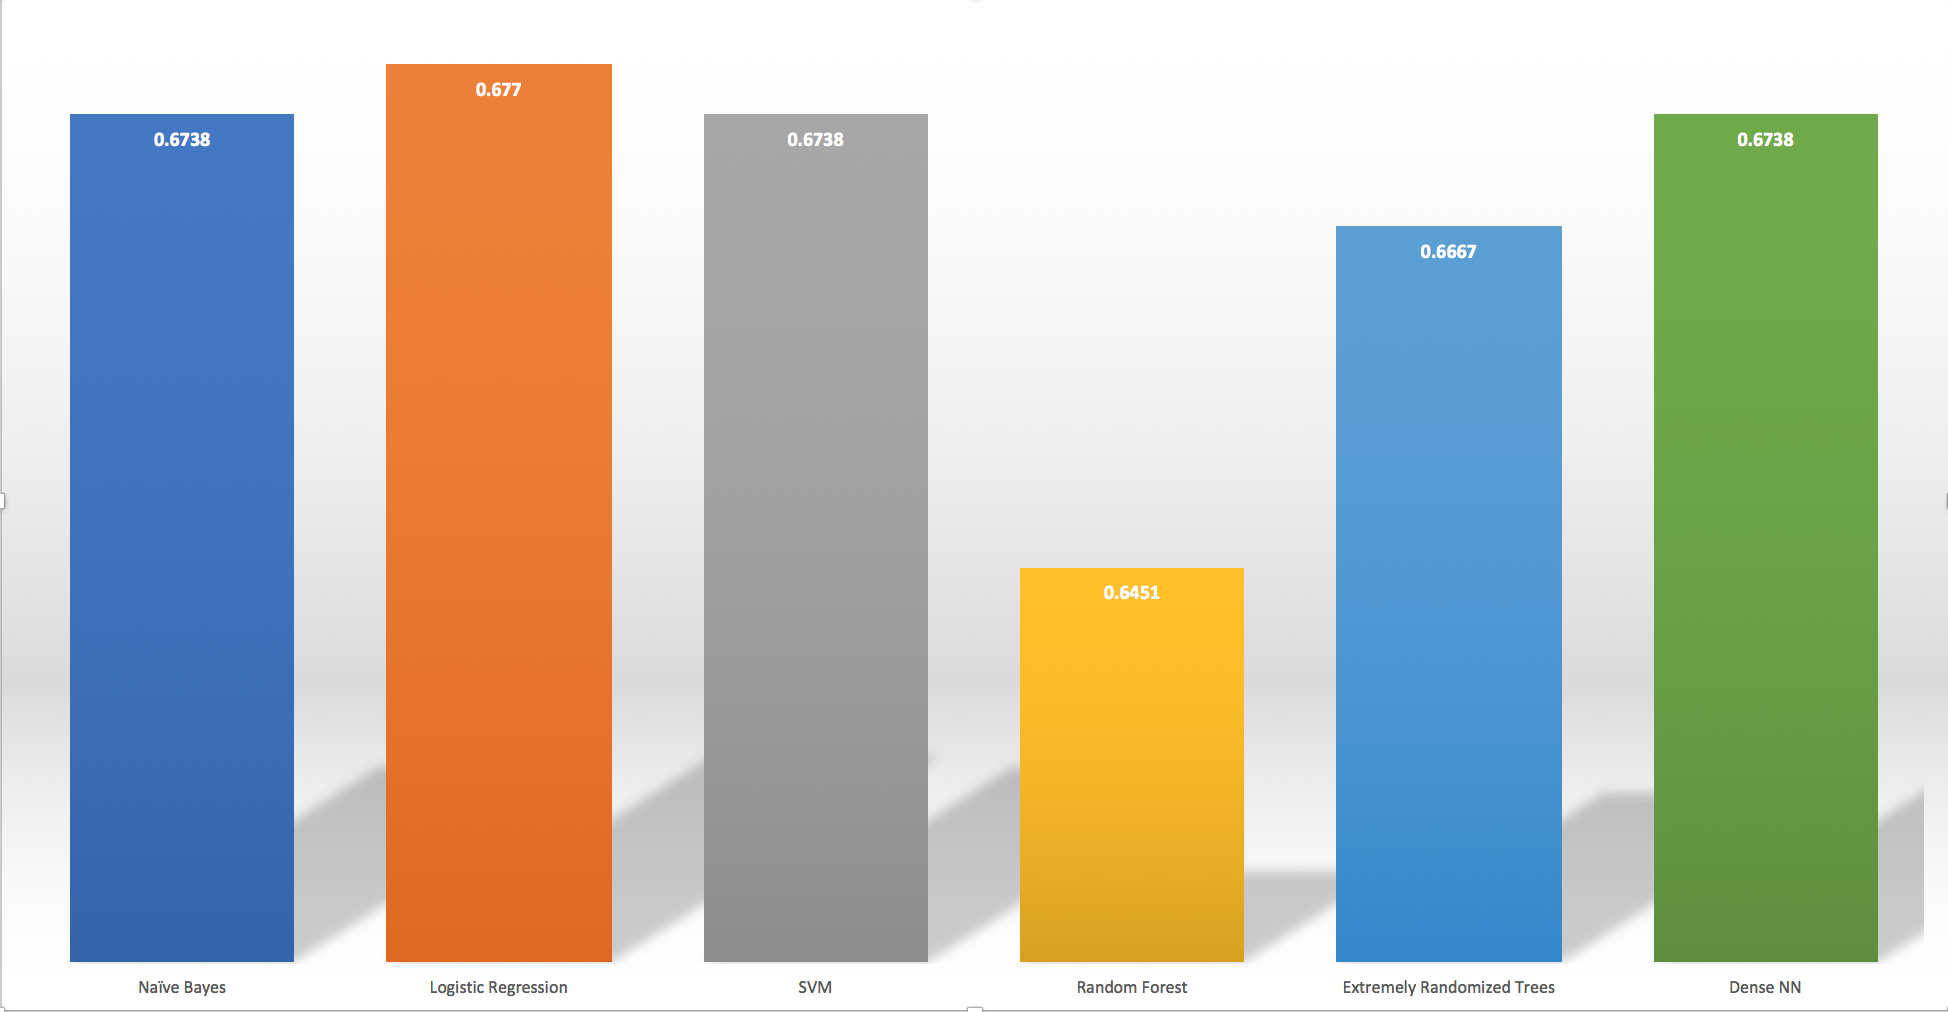
\includegraphics[scale=0.34]{images/comparison_algo_50.png}
\caption{Споредба на резултати од тестирање за податочно множество 50}
\label{fig:comparison_50}
\centering
\end{figure}


\section{Нулта точност}
Секогаш кога користиме класификациска точност, важно е да да ја споредиме со нулта точност. Нулта точност е точноста што може да ја постигниме со тоа што секогаш ќе ја предвидуваме најфреквентната класа во тест множеството. Ако ја пресметаме нултата точност за нашите податочни множества ќе видеме зошто ова е важна мeтрика. Кај множеството 49 имаме нулта точност од 45.52\% на класата 1, а кај можеството 50 имаме 54.48\% на класата Х2. На слика \ref{fig:null_acc_49} можеме да ја видеме споредбата на нултата точност во однос на другите алгоритми кај множеството 49, а на слика \ref{fig:null_acc_50} кај множеството 50. Од резултатите можеме да забележеме дека моделот на невронските мрежи и во двата случаи повторно ни дава добри резултати, за множеството 49 моделот е подобар за 10.4\%, а за множеството 50 за 12.9\%. Исто така овде многу добри резултати ни покажа и моделот на екстремно случајни дрва каде и во двата случаи резултатот од предвудувањата е подобар од нултата точност за 12.18\%.
\begin{figure}[H]
\centering
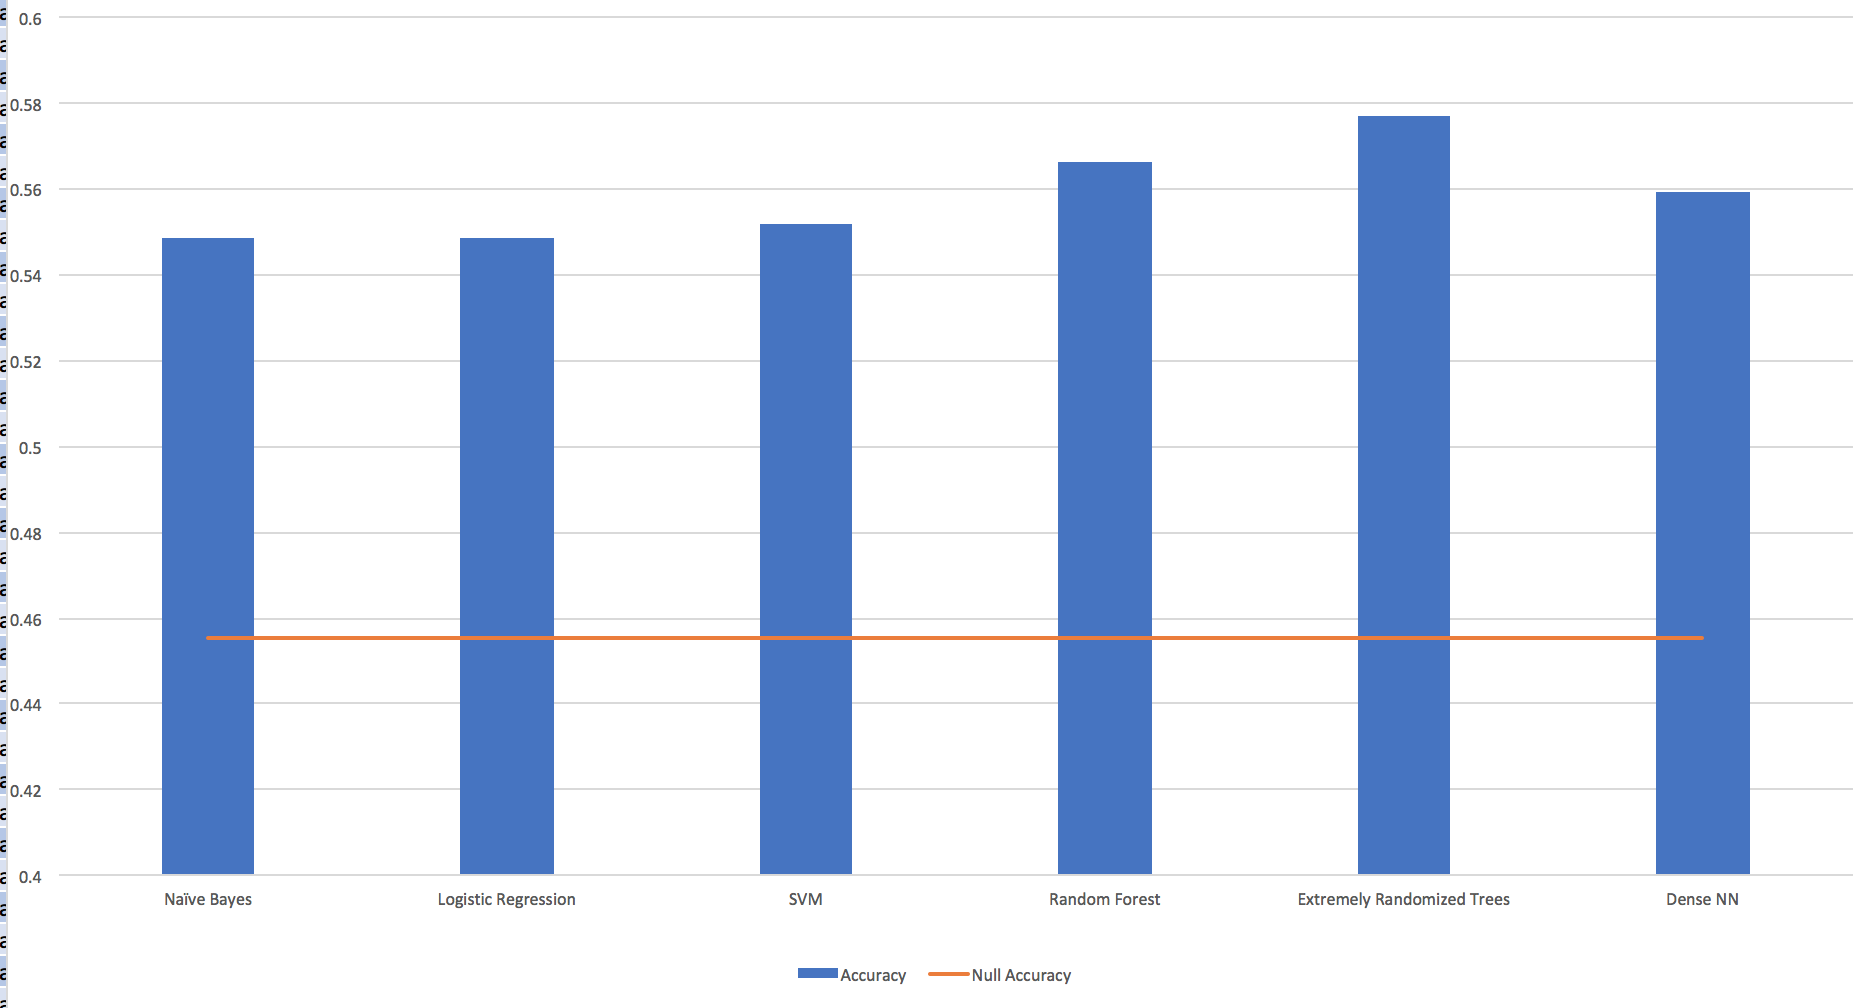
\includegraphics[scale=0.34]{images/null_accuracy_49.png}
\caption{Споредба на резултати од тестирање со нулта точност за податочно множество 49}
\label{fig:null_acc_49}
\centering
\end{figure}

\begin{figure}[H]
\centering
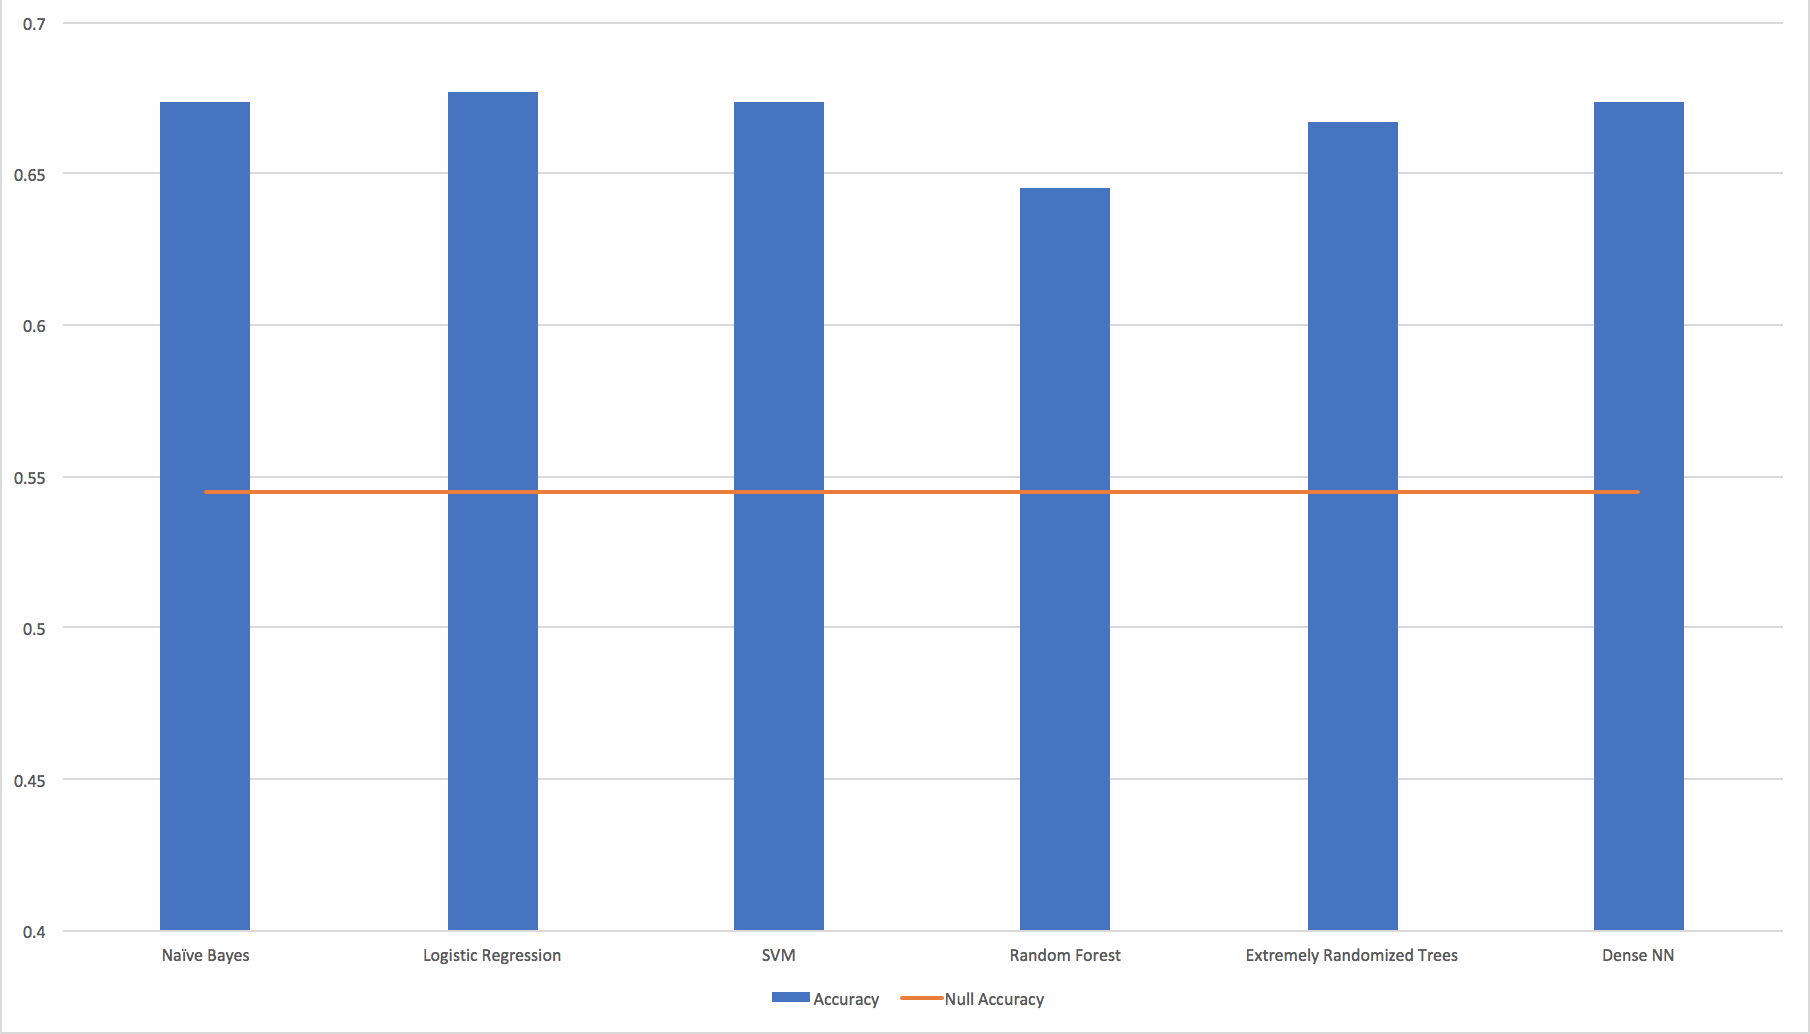
\includegraphics[scale=0.34]{images/null_accuracy_50.png}
\caption{Споредба на резултати од тестирање со нулта точност за податочно множество 50}
\label{fig:null_acc_50}
\centering
\end{figure}

\section{Матрица на забуни}
Матрицата на забуни е табела која ги опишува перформансите на еден класификацискиот модел. Матрицата е со големина k*k каде k е бројот на класи. 
\begin{table}[H]
 \centering
 \scalebox{0.8}{%
 \begin{tabular}{| c | c | c |}
 \hline
 & Предвидено = 0 & Предвидено = 1 \\
  \hline
 Реално = 0 & TN & FP \\
 Реално = 1 & FN & TP \\
 \hline
\end{tabular}}
\caption{Пример на матрица на забуни}
\label{table:confusion_mat_example}
\end{table}

На табела \ref{table:confusion_mat_example} е прикажана матрица на забуни за бинарен проблем, и кога се користи за ваков тип на класификација секој елемент од матрицата има специфично име:
\begin{itemize}
  \item Точно позитивно (True Positive, TP анг,): Броjот на точни придвидувања дека инстанцата е позитивна.
  \item Точно негативно (True Negative,TN анг.): Броjот на точни предвидувања дека инстанцата е негативна.
 \item Неточно позитивно (False Positive, FP анг.): Броjот на неточни предвидувања дека инстанцата е позитивна.
 \item Неточно негативно (False Negative, FN анг.): Броjот на неточни предвидувања дека инстанцата е негативна.
\end{itemize}
Матрицата на забуни се користи за да ни помогне подобро да ја разбереме работата на нашиот модел, но од неа директно не можеме да одбериме кој модел е подобар, бидејќи не е метрика за евалуација на модел. Како и да е, постојат метрики кои можат да бидат пресметани од матрица на забуни, и тие може директно да се искористат да се одбере најдобар модел. Ќе разгледаме неколку од популарните метрики и на крај ќе одбереме која метрика да ја оптимизираме.

Една од наједноставните и најочигледните метрики што можеме да ги пресметаме со матрица на забуни е точноста претставена како:
\begin{equation}
\frac{TP + TN}{TP + FP + FN + TN}
\end{equation}
Следната метрика е рата на грешка односно колку често класификаторот направил погрешно предвидување:
\begin{equation}
\frac{FP + FN}{TP + FP + FN + TN}
\end{equation}

Рата на точно позитивно предвидување или уште познато како осетливост (sensitivity, recall, hit rate, or true positive rate, анг.):

\begin{equation}
TPR = \frac{TP}{TP + FN}
\end{equation}

Рата на неточно позитивно предвидување (false positive rate оr fall-out, анг.):

\begin{equation}
FPR = \frac{FP}{TN + FP}
\end{equation}

Рата на точно негативно предвидување (specificity or true negative rate, анг.):

\begin{equation}
TNR = \frac{TN}{FP +TN}
\end{equation}

Рата на неточно негативно предвидување или промашување (miss rate or false
negative rate анг.):

\begin{equation}
FNR = \frac{FN}{FN + TP}
\end{equation}


Прецизност (precision or positive predictive value, анг.), односно колку често предвидениот излез е точен:
\begin{equation}
\frac{TP}{TP + FP}
\end{equation}

Доколку броjот негативни случаи е значително поголем од броjот на позитивни случаи, тогаш овие пресметки ќе посочат каде настанува грешка.
Во нашите случаи исто така ги применивме горните равенки за да ги најдеме дополнителните метрики кои ќе ни требаат за следниот чекор а тоа е градење на стратегија на обложување. Метриките за множество 49 и множество 50 се прикажани на табела \ref{table:metrics_49} и табела \ref{table:metrics_50} соодветно.

\begin{table}[H]
 \centering
 \scalebox{0.5}{%
 \begin{tabular}{| c | c | c | c | c | c | c | c | c |}
 \hline
 класификатор & точност & рата на грешка & осетливост 1 & осетливост X & осетливост 2 & прецизност 1 & прецизност X & прецизност 2 \\
  \hline
 NaiveBayes & 0.5483 & 0.4516 & 0.5467	& 0 & 	0.8819 & 0.4940 &	0 &	0.5714\\
 LogisticRegression & 0.54838 & 0.4516 & 0.8740 & 0.56 & 0.0 & 0.5663 & 0.5060 & 0.0\\
 SVM & 0.5519& 0.4480 & 0.8740 & 0.5733 & 0.0 & 0.5692 & 0.5119 & 0.0 \\
 RandomForest & 0.5663 & 0.4336 & 0.7637 & 0.5733 & 0.2337 & 0.6024 & 0.5243 & 0.5 \\
 ExtremelyRandomizedTrees & 0.5770 & 0.4229 & 0.8031 & 0.56 & 0.2207 & 0.5964 & 0.5675 & 0.5\\
 NeuralNet & 0.5591 & 0.4408 & 0.8661 & 0.0649 & 0.5466 & 0.5555 & 0.7142 & 0.5540 \\
 \hline
\end{tabular}}
\caption{Изведени метрики од матрица на забуни за множество 49}
\label{table:metrics_49}
\end{table}

\begin{table}[H]
 \centering
 \scalebox{0.8}{%
 \begin{tabular}{| c | c | c | c | c |}
 \hline
 класификатор & точност & рата на грешка & осетливост & прецизност \\
  \hline
 NaiveBayes & 0.6451 & 0.3548 & 0.6535 & 0.6014 \\
 LogisticRegression & 0.6774 & 0.3225 & 0.5511 & 0.6796 \\
 SVM & 0.6738 & 0.3261 & 0.5039 & 0.6956 \\
 RandomForest & 0.6738 & 0.3261 & 0.5196 & 0.6875 \\
 ExtremelyRandomizedTrees & 0.6666 & 0.3333 & 0.5354 & 0.6666 \\
 NeuralNet & 0.6738 & 0.3261 & 0.5039 &  0.6956 \\
 \hline
\end{tabular}}
\caption{Изведени метрики од матрица на забуни за множество 50}
\label{table:metrics_50}
\end{table}

Добра практика е секогаш да ја испитуваме матрицата на забуни бидејќи ни дава целосна слика колку е ефикасен нашиот класификатор. Исто така ни дозволува да пресметаме различни класификациски метрики кои може да не насочат кон одбирање на подобар класификациски модел. 

\section{Стратегија}

Откако ја анализиравме точноста на моделите и метриките што се изведуваат од матрицата на забуни, можеме да предложиме стратегија за максимизирање на добивката на корисниците на нашиот систем. Просечниот обложувач претежно се обложува на повеќе натпревари на еден влог со надеж дека тоа ќе ја зголеми неговата добивка. Обложувалниците со тоа нудат зголемување на квотата на уплатата со тоа што вкупната квота што ја добива обложувачот е производ од сите квоти за кои тој типува и добивката изгледа примамлива. Со ваквиот начин на уплата од друга страна се намалува веројатноста на добивка. Од надежност на системи \cite{fussell1975hand} познато е дека доколку имаме повеќе компоненти во системот, во нашиот случај типувања на натпревари, надежноста на системот се намалува, пресметана со,

\begin{equation}
P= P_1\\P_2\\...P_n
\end{equation}

 каде n е бројот на компоненти на системот, а P\textsubscript{x} е надежноста на компонентата. Поради ваквата поставеност, нашата стратегија се базира на посебен влог на секое типување и со тоа шансата на загуба зависи само од една компонента. Резултатите од симулациите што ги направивме се прикажани на табела \ref{table:win_sim_49} и табела \ref{table:win_sim_50}. Од резултатите можеме да забележиме дека кај множесвото 50 за сите модели добиваме позитивни резултати.
 
  \begin{table}[H]
 \centering
 \scalebox{0.8}{%
 \begin{tabular}{| c | c |}
 \hline
 класификатор & добивка \\
  \hline
 NaiveBayes & -3.15\%  \\
 LogisticRegression & -5.19\%  \\
 SVM & -11.68\%  \\
 RandomForest & +4.67\% \\
 ExtremelyRandomizedTrees & -3.04\% \\
 NeuralNet & -3.04\%  \\
 \hline
\end{tabular}}
\caption{Симулација на добивка за множеството 49}
\label{table:win_sim_49}
\end{table}
 
 \begin{table}[H]
 \centering
 \scalebox{0.8}{%
 \begin{tabular}{| c | c |}
 \hline
 класификатор & добивка \\
  \hline
 NaiveBayes & +1.6\%  \\
 LogisticRegression & +2.83\%  \\
 SVM & +1.8\%  \\
 RandomForest & +2.23\% \\
 ExtremelyRandomizedTrees & +2.2\% \\
 NeuralNet & +1.6\%  \\
 \hline
\end{tabular}}
\caption{Симулација на добивка за множеството 50}
\label{table:win_sim_50}
\end{table}

\section{Прилагодување на прагот на класификација}

За да ја подобриме добивката на системот треба да ги погледнеме метриките изведени од матрицата на забуни и како би ни користеле во нашиот случај. Изборот на метриката на која сакаме да оптимизираме зависи од нашата бизнис цел, дали сакаме да ја оптимизираме презицноста на нашиот модел или осетливоста. Кај еден ваков систем на препораки целта е да се намалат неточните позитиви (false positive анг.), затоа ќе се фокусираме кон зголемувањето на прецизноста на нашиот модел. За да ја зголемиме прецизноста на моделите го зголемуваме прагот на класификација, со тоа класата ќе биде препознаена доколку го надмине прагот кој ќе го поставиме. Доколку ниедна класа не го надминува поставениот праг, тој натпревар нема да го земеме во предвид. На слика \ref{fig:thresh_simulation_50} е прикажан графикот од симулацијата на множеството 50, за различни прагови и вкупната добивка изразена во проценти. На табела  \ref{table:win_sim_50_0_8} е претставена финалната симулација и потенцијалните добивки од ваквиот систем. Од резултатите можеме да заклучиме дека со зголемувањето на прагот на класификација забележуваме раст на добивката. 

\begin{figure}[H]
\centering
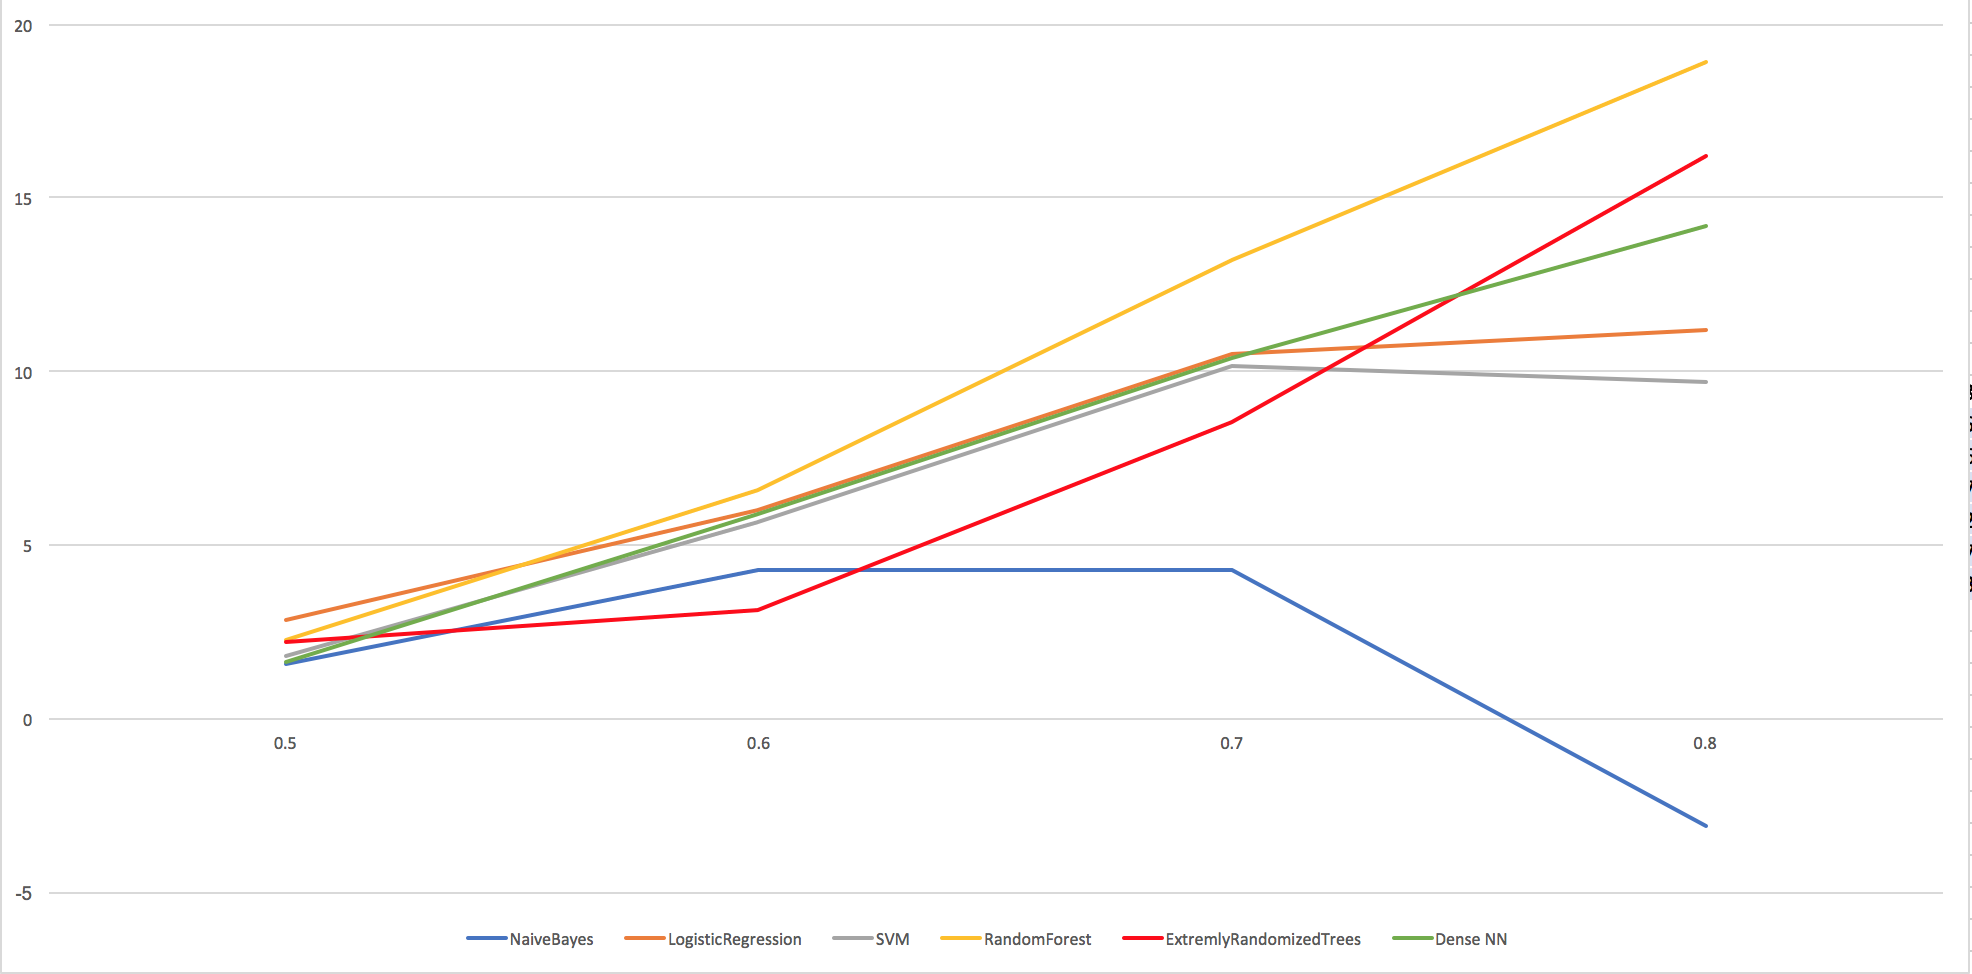
\includegraphics[scale=0.34]{images/thresh_simulation_50.png}
\caption{Симулација на добивка по различни прагови за множество 50}
\label{fig:thresh_simulation_50}
\centering
\end{figure}

 \begin{table}[H]
 \centering
 \scalebox{0.8}{%
 \begin{tabular}{| c | c |}
 \hline
 класификатор & добивка \\
  \hline
 NaiveBayes & -3.08\%  \\
 LogisticRegression & +11.21\%  \\
 SVM & +9.67\%  \\
 RandomForest & +18.89\% \\
 ExtremelyRandomizedTrees & +16.21\% \\
 NeuralNet & +14.20\%  \\
 \hline
\end{tabular}}
\caption{Симулација на добивка за множеството 50 со праг на класификација од 0.8}
\centering
\label{table:win_sim_50_0_8}
\end{table}

\section{Исплатливост}

Со моделите на случајни шуми, екстремно случајни дрва и невронските мрежи забележувме значителна добивка. За споредба банкарските камати на орочување од 1 до 5 години се движат од 1.2\% до 3.6\%, додека нашиот систем произведува заработка од 14\% до 18\% од целосниот влог. Сепак овој начин на заработка е доста ризичен и не можеме да го одобриме и покрај добрите резултати.

\chapter{Заклучок и идна работа}
\label{sec:conclusion}

Во овој магистерски труд главна тема беше предвидувањето на резултати од спортски натпревари со помош на алгоритми за машинско учење, каде главниот фокус беа на невронските мрежи. Дознавме дека за да се направи успешен систем за препораки се потребни повеќе процеси кои беа разгледани во текот на ова истражување.

Во глава \ref{sec:architecture} беше разгледана архитектурата на системот за препораки, каде поминавме низ процесот на дизајнирање на системи. Ги разгледавме кои се корисничките сценарија и огранучувањата на еден ваков систем. Беше понуден апстрактен дизајн на системот и подобрувања за справувања со тесни грла. Со ова се доби јасна претстава кои се најпотребните компоненти за еден ваков систем да работи.

Во глава \ref{sec:data} беа обработени две кориснички сценарија превземање и обработка на податоците. Покажано беше дека за еден ваков систем да работи пред сè се потребни податоци, но потребни се добри податоци. При обработката на податоци беа применети неколку техники за промена на податоците и податочното множество со цел да добиеме подобри резултати во следните чекори.

Во глава \ref{sec:machine_learning} беа разгледани повеќе алгоритми за машинско учење кои служеа како репер за вештачките невронски мрежи. Разгледани беа алатките потребни за креирање на модел за вештачки невронски мрежи и техники за добивање на најдобрите параметри и најдобрата архитектура. Беше претставена густо поврзаната невронска мрежа како архитектура која најдобро го решава проблемот на функциско мапирање и како овој алгоритам се справува со проблемот во однос на другите алгоритми.

Во глава \ref{sec:evaluation} се направи евалуација на разултатите од моделите на класификација. Овде беше покажано дека кај еден класификациски модел не е доволно само тренирање и тестирање на податоците и со тоа добивање на точност. Прво, беа споредени резутатите со нултата точност да се види дали моделите добро го решаваат проблемот. Беше разгледана матрицата на забуни како алатка која дава целосна слика на еден класификациски модел и од која може да се изведат дополнителни метрики кои може да се оптимизираат со цел да се постигне одредена бизнис цел. На крај беше изградена стратегија на системот и беше оптимизирана со помош на метриките од матрицата на забуни. Со тоа беше максимизиран профитот на потенцијалните корисници на системот.

Во денешно време освен обложувањето на спортски натпревари, постојат постојат повеќе места на кои луѓето гледаат како начин на брза заработка на пари. Таков пример се берзите за криптовалути.

